\documentclass{article}
\usepackage{siunitx}
\usepackage{indentfirst}
\usepackage{graphicx}
\usepackage{amsmath}
\usepackage{float}
\usepackage[utf8]{inputenc}
\usepackage{wrapfig}
\usepackage{amstext}
\usepackage{commath}
\usepackage{listings}
\usepackage{caption}
\usepackage{subcaption}

\title{Theoretical and Experimental Findings in Weakly-Produced Supersymmetry: Exploring Long-Lived SUSY with a Compressed Mass Spectrum}
\author{Alexander Albert}
\date{August 2022}

\begin{document}
\maketitle
\newpage
\tableofcontents
\newpage
\section{Notes on Document Organization}
In this note, I've documented my knowledge of both the theoretical and experimental facets of supersymmetry (SUSY). In the first section, which I wrote for the final project of my undergraduate particle physics course, I summarize the hierarchy problem, describe how SUSY provides an elegant solution that appeals to ``naturalness", and motivate weakly-produced SUSY as a particularly interesting sector of SUSY worthy of further investigation. The second section provides a summary of a study on electroweak SUSY I worked on, led by postdoc Joey Reichert. If the experimental study is of predominant interest, I strongly encourage skipping the theoretically-oriented section.
\section{Theoretical Basis of SUSY as a Response to the Hierarchy Problem}
\subsection{Introduction and Motivations}
The discovery of the Higgs Boson at the Large Hadron Collider (LHC) in 2012 was one of the most influential events within the particle physics community. Coined the ``God Particle"  by the media, the Higgs Boson temporarily completed the Standard Model, providing experimental verification of the Higgs Mechanism, the phenomenon that gives mass to the weak force carriers, the W$\pm$ and Z bosons. The Higgs Mechanism is motivated by spontaneous symmetry-breaking, in which an initial ground state, a vacuum, lacks the same symmetry as the Lagrangian, which is determined by the ``sombrero"  potential for scalar fields, the Higgs potential [1]. I'll refrain providing a more mathematical and rigorous motivation to the Higgs Mechanism and spontaneous-symmetry breaking, as it is not the focus of this paper. However, it suffices to say that without the Higgs Boson, there would not exist a means for gauge bosons to acquire mass, which would contradict experimental findings of the mass of the W$\pm$ and the Z.
\par
The mass of the Higgs Boson was found to be ~125 GeV. In the context of particle physics, this is rather heavy. The W$^{\pm}$ bosons have a mass of 80 GeV, the Z boson has a mass of 91 GeV, and the heaviest lepton, the Tau, only weighs 1777 MeV [2]. However, the experimental mass of the Higgs introduces an array of inconsistencies to our understanding of the Standard Model, and is problematic with regards to other physical frameworks, such as gravity. The Hierarchy Problem is one such interesting open question. The Higgs Mechanism is inextricably tied with the our understanding of the weak interaction, and thus we expect the mass of the Higgs Boson to be related to G$_{f}$, the Fermi Constant that defines the strength of the weak force [3]. Therefore, we expect our measurement of the Higgs Mass, m$_{H}$, to be consistent with:
\begin{equation} \label{eq:1}
\frac{G_{f} \hbar^{2}}{G_{N} c^{2}},
\end{equation}
where $G_{N}$ is the Newton's Gravitational Constant [3]. Equation~\ref{eq:1} and $G_{N}$ are known, so we expect that the Higgs Mass should follow suit. However, the measured mass is far smaller than this prediction would suggest. The discrepancy can be attributed to quantum corrections to Feynman Diagrams that describe the behavior of the Higgs. I'll more robustly discuss the mathematical nature of these corrections in Section 2.
\par
Supersymmetry (SUSY) is an appealing and promising extension to the Standard Model that introduces an additional set of quantum corrections to the Higgs model. These ``new" corrections cancel out the existing quantum divergences mentioned above, such that the small Higgs Mass measured at the LHC is both viable and expected. According to SUSY, to properly motivate these calculations, there must exist a set of particles, currently unobserved in an accelerator, that create a symmetry between fermion and boson states in the Standard Model [4]. Appealing to a familiar Quantum Mechanical framework, this means that there exists some operator Q such that (from [4]):
\begin{equation} \label{eq:2}
Q|\text{Fermion}> = |\text{Boson}>, Q|\text{Boson}> = |\text{Fermion}>
\end{equation}
\par
However, for a given fermion state to satisfy Equation~\ref{eq:2}, the existence of Q must be accompanied by a boson of spin 1/2. Similarly, there must exist fermions of spin 0. As a result, supersymmetry introduces ``superpartners"  to the familiar Standard Model particles. Each spin 1/2 quark has a spin 0 ``squark"  superpartner, spin 1/2 electrons have a spin 0 superpartner ``selectron", and so on.
\par
In this paper, I'll introduce and formalize the importance and properties of ``electroweakinos", the superpartners to Standard Model bosons that carry the electromagnetic and weak interactions in the Minimal Supersymmetric Standard Model (MSSM). Weakly-produced SUSY predicts a variety of Feynman Diagrams that introduce unique signals that experimentalists could encounter at particle colliders. The electroweak SUSY sector consists of chargeless neutralinos ($\tilde{\chi}^{0}_{1,2,3,4}$) and charged charginos ($\tilde{\chi}^{\pm}_{1,2}$). The subscripts refer the mass hierarchy of the given particle; $\tilde{\chi}^{0}_{1}$ is the lightest neutralino, while $\tilde{\chi}^{0}_{4}$ is the heaviest. Neutralinos and charginos are the mass eigenstates of the mass matrix, and consist of a mixture of weak eigenstates, which determine whether a given electroweakino is ``Wino-like", ``Bino-like", or ``Higgsino-like"  [4]. The process of mixing the weak eigenstates is akin to the spontaneous symmetry breaking in the Standard Model, in which weak gauge bosons acquire mass after ``eating"  the Goldstone bosons. I'll discuss SUSY as a means of correcting the Hierarchy Problem and explore the properties of electroweakinos in Section 3.
\par
I hope that it is not troubling that I begin my report by discussing broad concepts and inconsistencies of the Standard Model before plunging into a rather narrow rabbit hole regarding a specific sector of supersymmetry. I instead could have written this report on a particular SUSY decay or only the mixing of the mass eigenstates, but I feel as though it is more instructive to motivate these esoteric topics in response to the current state of the Standard Model. I also believe that it is important to view new theory, such as SUSY, in conjunction with existing and well-understood calculations that should be familiar. As a result, the later topics in this paper will be presented analogously with Standard Model processes, which should provide a particularly instructive means of presenting unfamiliar phenomena.
\subsection{The Hierarchy Problem}
At an undergraduate level, we focused mainly on tree diagrams when computing scattering amplitudes and related attributes. The quantum corrections to the Higgs mass, however, are a result of loop diagrams. For the Higgs, the total contribution from Loop diagrams can be derived by summing over the contributions from self-interactions, gauge loops, and fermion loops, described pictorially in Figure~\ref{fig:1} [5]. 
\begin{figure}[H]
    \centering
    \caption{} 
    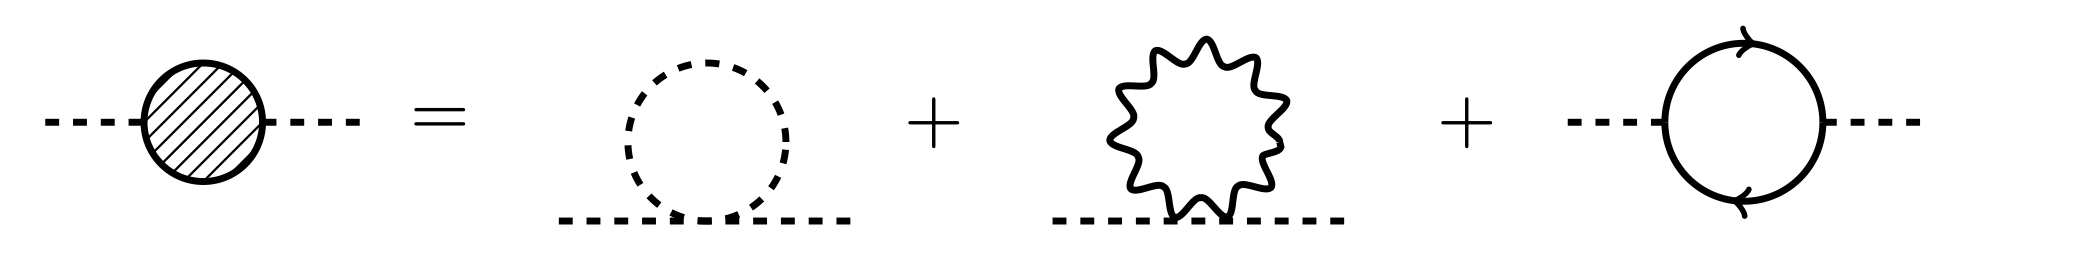
\includegraphics[width=12cm]{Loops.png}
    \label{fig:1}
\end{figure}
\par
Loop diagrams often introduce divergent corrections, i.e, the integrals used to evaluate amplitudes do not converge to a finite value, which is why we largely avoided them in the course. This complication can usually be ameliorated by introducing a factor inside the integral that includes a cutoff mass M, such that the integral now evaluates to a finite value [1]. In order to maintain self-consistency within our theory, we modify our effective masses and coupling constants so that [1]:
\begin{equation}\label{eq:3}
    \begin{aligned}    
    & m_{physical} = m + {\delta}m \\
    & g_{physical} = g + {\delta}g
    \end{aligned}
\end{equation}
The value 'm' is derived from tree-level computations. The $\delta$m introduces the divergent corrections that disagree with experimental values of the Higgs mass.
\par
Suppose we want to reconcile the physics from our scalar Higgs field with an energy regime in which new physics occurs. An example would be the energy at which the electromagnetic and weak interaction recombine. Let S be a scalar that exists at this higher energy. We denote the cutoff value for renormalization $\Lambda_{uv}$ and the coupling between the Higgs and the complex S (which consists of two real scalar fields combined as, $\phi_{1}$ + i$\phi_{2}$) as $\lambda_{s}$. The correction term becomes [5]:
\begin{equation} \label{eq:4}
    {\delta}m_{h}^{2} = \frac{{\lambda}_{s}}{16\pi^{2}}[\Lambda_{uv}^{2}-2m_{s}^{2}ln(\frac{\Lambda_{uv}}{m_{s}}) + (\text{finite})]
\end{equation}
\par
Similarly, let f be a fermion. The correction term from the fermion loop is of the form:
\begin{equation} \label{eq:5}
    {\delta}m_{h}^{2} = -\frac{{\lambda}_{f}}{16\pi^{2}}[\Lambda_{uv}^{2}-2m_{f}^{2}ln(\frac{\Lambda_{uv}}{m_{f}}) + (\text{finite})]
\end{equation}
\par
These results are deeply concerning when considered independently. Let's focus on the $\Lambda_{uv}^{2}$ term, the quadratic divergence. Physically, this says that the mass corrections depends on the energy scale with which we want to introduce new physics! If we want to unify the strong, weak, and electromagnetic forces with gravity, we set our parameter $\Lambda_{uv}$ to the appropriate energy scale. By construction, the Plank scale allows these interactions to coexist, but prescribes energy scales of ~10$^{19}$ GeV. Again, since the Higgs mass is measured to be ~125 GeV, the discrepancy is immense. Furthermore, the Higgs Mass depends on whether its field is coupling with a fermion or with another scalar. However, Equation~\ref{eq:4} and Equation~\ref{eq:5} are of very similar forms, which suggests a potential symmetry between fermions and scalars.
\par
Therefore, it becomes necessary to look for a means to expand the Standard Model and eliminate this inconsistency. More broadly, we need to reimagine our physical framework so that physical constants, such as the Higgs mass, are independent of scale.
\subsection{Minimal Supersymmetric Standard Model (MSSM)}
\subsubsection{Cancelling Quadratic Divergences with a New Lagrangian}
The standard Yukawa Lagrangian for a scalar field $\phi$ and a spin-1/2 Dirac Particle and Antiparticle $\psi$ is [1]:
\begin{equation} \label{eq:6}
    {\mathcal{L}} = [i{\hbar}c\Bar{\psi}{\gamma^{\mu}}{\partial_{\mu}}\psi - m_{1}c^{2}\Bar{\psi}{\psi}] + [\frac{1}{2}(\partial_{\mu}\phi)(\partial^{\mu}\phi) - \frac{1}{2}(\frac{m_{2}c}{\hbar})^{2}] - {\lambda}_{Y}\Bar{\psi}\psi{\phi}
\end{equation}
\par
Here, the interaction between the Higgs field and the fermion (Dirac spinor) is embedded in the last term in Equation~\ref{eq:5}, $\lambda_{Y}\Bar{\psi}\psi{\phi}$. However, this Lagrangian exists for a field theory that consists of only a scalar field that couples to a Dirac particle. Under SUSY, this structure is incomplete, and we posit that there exists another symmetry that modifies our Lagrangian.
\par
We follow the procedure taken by [6] to find a new Lagrangian that is invariant under fermion $\rightarrow$ boson transformations, and vice versa. Source [6] covers this procedure in more rigor than I am here, and should be consulted if necessary. A Lagrangian invariant under this transformation ensures that whenever we consider fermion loop corrections, there must exist some mechanism that creates a boson loop correction, cancelling the problematic quadratic divergences described in the previous section.
\par
Under SUSY, we can group Standard Model particles with their superpartners within an mathematical object known as a supermultiplet. Supermultiplets operate in a very similar way to spinors. One such object is the chiral supermultiplet, which consists of a spin-1/2 Standard Model particle and its spin-0 superpartner, which is represented by a complex scalar field. For example, the electron, electron neutrino, selectron, and selectron neutrino form a supermultiplet, with the selectron and selectron neutrino together forming a spin-0 complex scalar field.
\par
Let's describe a chiral supermultiplet via a Lagrangian. For now, we ignore interaction terms and only worry about the kinetic energies for spin-1/2 and spin-0 fields.
\begin{equation} \label{eq:7}
    \begin{aligned}
    & {\mathcal{L}} = {\mathcal{L}_{scalar}} + {\mathcal{L}_{fermion}} \\
    & {\mathcal{L}_{scalar}} = -\partial^{\mu}\bar{\phi}\partial_{\mu}\phi \\
    & {\mathcal{L}_{fermion}} = i\bar{\psi}\bar{\gamma^{\mu}}\partial_{\mu}\psi
    \end{aligned}
\end{equation}
\par
A SUSY transformation should map fermions to scalars and vice-versa, so we define some spinor $\epsilon$ such that:
\begin{equation} \label{eq:8}
    \begin{aligned}
    & \delta{\phi} = \epsilon{\psi} \\
    & \delta{\bar{\phi}} = \delta{\bar{\epsilon}}\bar{\psi} \\
    & \delta{\psi_{\alpha}} = -i(\gamma^{\mu}\bar{\epsilon})_{\alpha}\partial_{\mu}\phi \\
    & \delta{\bar{\psi}_{\dot{\alpha}}} = i(\epsilon{\gamma_{\mu}})_{\dot{\alpha}}\partial_{\mu}\bar{\phi}
    \end{aligned}
\end{equation}
\par
To maintain invariance of the Lagrangian under SUSY transformations, we require that [$\epsilon_{1}$, $\epsilon_{2}$]$\psi$ and [$\epsilon_{1}$, $\epsilon_{2}$]$\phi$ lead only to a ``spacetime"  transformation, i.e. one that is proportional to $\partial_{\mu}$ [6] This is because we should be able to apply fermion $\rightarrow$ boson transformations in whatever order we desire. We find that:
\begin{equation}. \label{eq:9}
    \begin{aligned}
        & [\epsilon_{1}, \epsilon_{2}]\phi = i(-\epsilon_{1}\gamma^{\mu}\epsilon_{2} + \epsilon_{2}\gamma^{\mu}\epsilon_{1})\partial_{\mu}\phi \\
        & [\epsilon_{1}, \epsilon_{2}]\psi = i(-\epsilon_{1}\gamma^{\mu}\epsilon_{2} + \epsilon_{2}\gamma^{\mu}\epsilon_{1})\partial_{\mu}\psi + i\epsilon_{1\alpha}(\bar{\epsilon_{2}}\bar{\gamma^{\mu}}\partial_{\mu}\psi) - i\epsilon_{2\alpha}(\bar{\epsilon_{1}}\bar{\gamma^{\mu}}\partial_{\mu}\psi) \\
    \end{aligned}
\end{equation}
\par
The equation for $\phi$ gives the desired relation. However, the second and third terms in the $\psi$ equation do not lead to invariance. We can fix this by introducing an additional scalar, spin-0 field F, to our system. To preserve the physics of our system, we ensure that F satisfies the equations of motion F = $\bar{F}$ = 0. As a result, we have new transformation rules:
\begin{equation} \label{eq:10}
    \begin{aligned}
    & \delta{\phi} = \epsilon{\psi} \\
    & \delta{\psi_{\alpha}} = -i(\gamma^{\mu}\bar{\epsilon})_{\alpha}\partial_{\mu}\phi + \epsilon_{\alpha}F \\
    & \partial{F}. = -i\bar{\epsilon}\bar{\gamma^{\mu}}\partial_{\mu}\psi
    \end{aligned}
\end{equation}
And a new Lagrangian:
\begin{equation} \label{eq:11}
    {\mathcal{L}} = -{\partial}^{\mu}\bar{\phi}\partial_{\mu}\phi + i\bar{\psi}\bar{\gamma^{\mu}}\partial_{\mu}\psi + \bar{F}F
\end{equation}
\par
We now satisfy $[\epsilon_{1}, \epsilon_{2}]\B = i(-\epsilon_{1}\gamma^{\mu}\epsilon_{2} + \epsilon_{2}\gamma^{\mu}\epsilon_{1})\partial_{\mu}{B}$ where B is $\phi$, $\psi$, or F. Therefore Equation~\ref{eq:11} is invariant under SUSY transformations for a given chiral supermultiplet. This property is particularly significant, because it posits the existence of a physical system with symmetry between the fermionic and bosonic contributions to physical phenomena. In other words, if the most basic building block of an effective field theory is a chiral supermultiplet, then said system is immune to the type of quadratic divergence that results from the fermion-boson asymmetry that brings about the Hierarchy Problem. Note that our procedure for proving the invariance of the Lagrangian in a system consisting of a chiral supermultiplet can be adapted to other supermultiplets that include gauge and theorized gravitational particles.
\par
We recall that we turned off interactions and couplings in the chiral supermultiplet system described by equation~\ref{eq:11}, so the result should be interpreted more as a proof-of-principle regarding SUSY invariance as opposed to a rigorous depiction of a plausible physical system. For the remainder of this paper, I'll specifically consider the MSSM SUSY model and its associated constituents. To complete the Lagrangian for a SUSY theory and reincorporate particle-particle interactions, we add potential terms that describe interactions between chiral fields and our gauge functions. MSSM is a particular model that specifies a ``superpotential"  that maintains an additional symmetry known as R-parity [5]. Under R-Parity, the lightest SUSY particle (LSP) is stable, and is thus considered a plausible candidate for dark matter and other mysterious phenomena [7]. For this reason, we choose MSSM as a particular model worthy of further exploration.
\subsubsection{Probing the Electroweak Sector of MSSM}
Thus far, our investigation of SUSY has been largely focused on the mathematical framework it provides as a means to solve the Hierarchy Problem. Now, we operate under the assumption that a SUSY framework can exist, and readjust our focus to better align with the attributes of SUSY that best lend itself to finding experimental evidence. Neutralinos and charginos (electroweakinos) are particularly useful in this regard, as will be apparent when we investigate the signal models that we expect searches at the LHC to be sensitive to.
\par
First however, I'll briefly explain how neutralinos and charginos act as a superposition of weak eigenstates, and how different superpositions can lead to different signal models and expected interactions. Let's first appeal to familiar Standard Model phenomena. We recall that charged weak interaction (those modulated by the W$\pm$) are defined by the CKM matrix [1]:
\begin{equation} \label{eq:12}
\begin{pmatrix}
    V$_{ud}$ & V$_{us}$ & V$_{ub}$ \\
    V$_{cd}$ & V$_{cs}$ & V$_{cb}$ \\
    V$_{td}$ & V$_{ts}$ & V$_{tb}$ \\
\end{pmatrix}
\end{equation}
\par
After plugging values into Equations~\ref{eq:12}, we can describe the identity of a quark after emitting a W$\pm$ by [1]:
\begin{gather} \label{eq:12}
\begin{pmatrix}
    d' \\
    s' \\
    b' \\
\end{pmatrix}
=
\begin{pmatrix}
    0.974 & 0.227 & 0.004 \\
    0.227 & 0.973 & 0.042 \\
    0.008 & 0.042 & 0.999 \\
\end{pmatrix}
\begin{pmatrix}
    d \\
    s \\
    b \\
\end{pmatrix}
\end{gather}
\par
Since the matrix is not perfectly diagonal, the ``generation"  of the quark is not necessarily conserved by the flavor-changing interaction. In other words, a down quark can decay to a charm or top quark, even though it's of the same generation of the up quark. Thus, the identity of the final state quark, denoted by the prime, is a probabilistic mixture of many different quark flavors.
\par
Let's apply the same idea to our electroweakinos. First, we recall that the weak bosons in the Standard Model acquire mass by ``eating"  the Goldstone bosons the Higgs mechanism provides [1]. In other words, if we start with four Goldstone Bosons, or ``little Higgses``, under spontaneous symmetry breaking, these bosons get ``mapped"  to the three weak-interaction bosons and the Higgs Boson. We can describe the analogous process in MSSM. Here, the Goldstone bosons correspond to the weak eigenstates, which consists of the the gauge field of the weak hypercharge known as the Bino ($\tilde{B}$), the W$\pm$ superpartner known as the Wino ($\tilde{W^{0}}$), and the two Higgsinos, which form a doublet ($\tilde{H_{d}^{0}}$ and $\tilde{H_{u}^{0}}$) [8]. The bosons that acquire mass via the Higgs mechanism are analogous to MSSM's four neutralinos. The transformation from the weak eigenstates to the neutralinos is given by the ``mass matrix"  [8]:
\begin{gather} \label{eq:13}
\begin{pmatrix}
    \tilde{\chi^{0}_{1}} \\
    \tilde{\chi^{0}_{2}} \\
    \tilde{\chi^{0}_{3}} \\
    \tilde{\chi^{0}_{4}}
\end{pmatrix}
\propto
\begin{pmatrix}
    M_{1} & 0 & -c_{\beta}s_{W}m_{Z} & s_{\beta}s_{w}m_{Z} \\
    0 & M_{2} & c_{\beta}c_{W}m_{Z} & -s_{\beta}c_{W}m_{Z} \\
    -c_{\beta}s_{W}m_{Z} & c_{\beta}c_{w}m_{Z} & 0 & -\mu \\
    s_{\beta}s_{W}m_{Z} & -s_{\beta}c_{w}m_{Z} & -\mu & 0 \\
\end{pmatrix}
\begin{pmatrix}
    \tilde{B} \\
    \tilde{W^{0}} \\
    \tilde{H_{d}^{0}} \\
    \tilde{H_{u}^{0}}
\end{pmatrix}
\end{gather}
\par
We hope to diagonalize the mass matrix so that we can determine the masses of our neutralinos by picking them off the diagonal [8]:
\begin{equation}\label{eq:14}
P^{-1}M_{\tilde{\chi^{0}}}P =
\begin{pmatrix}
    m_{\tilde\chi_{1}^{0}} & 0 & 0 & 0 \\
    0 & m_{\tilde\chi_{2}^{0}} & 0 & 0 \\
    0 & 0 & m_{\tilde\chi_{3}^{0}} & 0 \\
    0 & 0 & 0 & m_{\tilde\chi_{4}^{0}}
\end{pmatrix}
\end{equation}
\par
M$_{1}$ and M$_{2}$ come from the MSSM Lagrangian, while $\mu$ is the mass parameter for the Higgsino [8]. The other parameters are not particularly important in a qualitative sense. The exact values of these terms are not known, and as a result, we do not know whether our mass eigenstates, the neutralinos, are more Wino/Bino-like or Higgsino-like, and experimental searches must account for both cases. The Lighest Supersymmetric Particle (LSP) is the $\tilde\chi_{1}^{0}$, and if $\lvert$$\mu$$\rvert$ $\approx$ $\lvert$M$_{1}$$\rvert$ $\ll$ $\lvert$M$_{2}$$\rvert$ the LSP is Higgsino-like. If $\lvert$M$_{1}$$\rvert$ $\ll$ $\lvert$M$_{2}$$\rvert$ $\ll$ $\lvert$$\mu$$\rvert$, then the LSP is Wino/Bino like. In the next section, we'll discuss in greater detail the experimental distinction between these two cases.
\par
A similar mixing procedure occurs for the charginos. The masses can be found by solving the same eigenvalue problem for the corresponding mass matrix (remember, there are only two charginos in the mass hierarchy) [8]:
\begin{equation} \label{eq:15}
\begin{pmatrix}
    M_{2} & $\sqrt{2}$s_{\beta}m_{W} \\
    $\sqrt{2}$c_{\beta}m_{W} & \mu
\end{pmatrix}
\end{equation}
\section{Experimental Study in Weakly-Produced Long-Lived SUSY}
\subsection{Characteristics of Experimental Searches for MSSM Electroweakinos}
Let's investigate the theoretically-motivated SUSY processes that could be discovered or excluded at the LHC. Figure~\ref{fig:2} shows signal models that scientists at the Compact Muon Solenoid (CMS) detector at CERN are particularly interested in [9].
\begin{figure}[H]
    \centering
    \caption{} 
    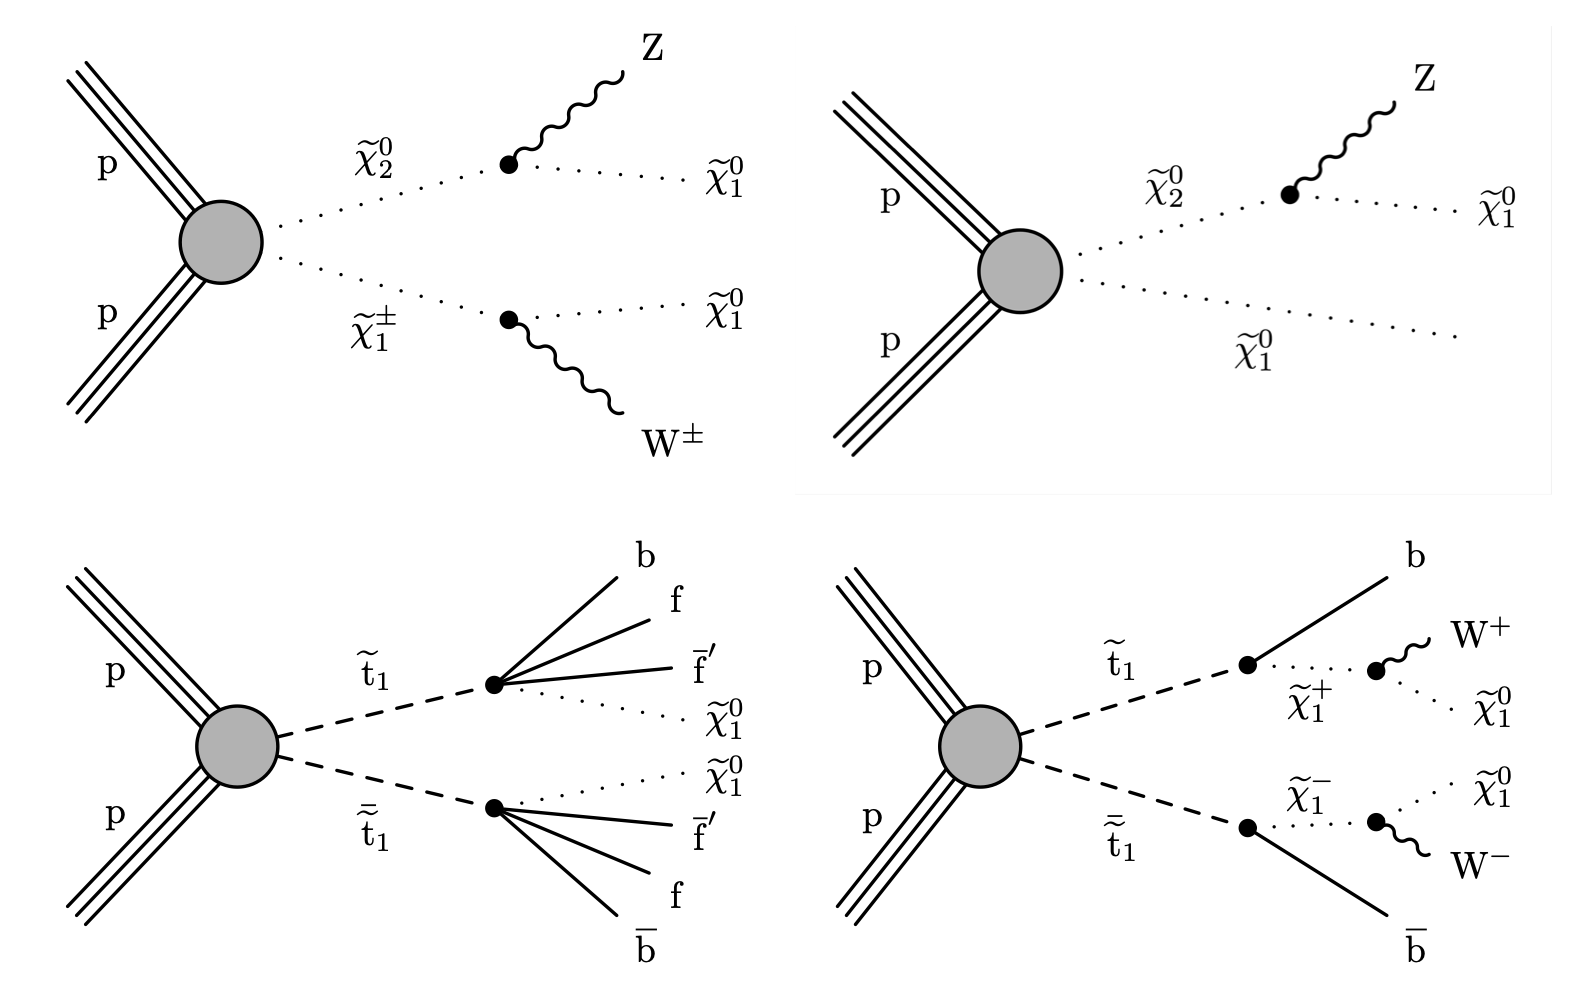
\includegraphics[width=12cm]{FeynmanDiagrams.png}
    \label{fig:2}
\end{figure}
\par
These particular processes bring about Standard Model final-state particles that detectors should be sensitive to. For the remainder of this paper, I'll focus on the top two diagrams, which are restricted to the electroweak sector of SUSY.
\par
Since neutralinos are chargeless, they do not interact with the silicon tracker or the electromagnetic calorimeter of the detector. As a result, direct detection of the LSP is nearly impossible. Experimental searches focus on the detecting the lepton decay products of the Z boson. Note that here the Z boson is off-shell, i.e. its mass is likely less than 91 GeV. This is because its mass is bounded above by the mass splitting of the neutralino 2 and the neutralino 1, or m$_{Z^{*}}$ $\leq$ m$_{\tilde\chi_{2}^{0}}$ - m$_{\tilde\chi_{1}^{0}}$. As a result, the lepton decay products themselves are lighter than their rest mass. However, for a given choice of electroweakino masses and mass splittings, the kinematic properties of the Z and its decay products can be simulated with great precision. It should be noted that muons are the easiest lepton to detect experimentally, as detectors such as CMS usually include muon ``chambers"  that can reconstruct muon tracks very well. Figure~\ref{fig:3} shows a cross-sectional diagram of the CMS detector [10].
\begin{figure}[H]
    \centering
    \caption{} 
    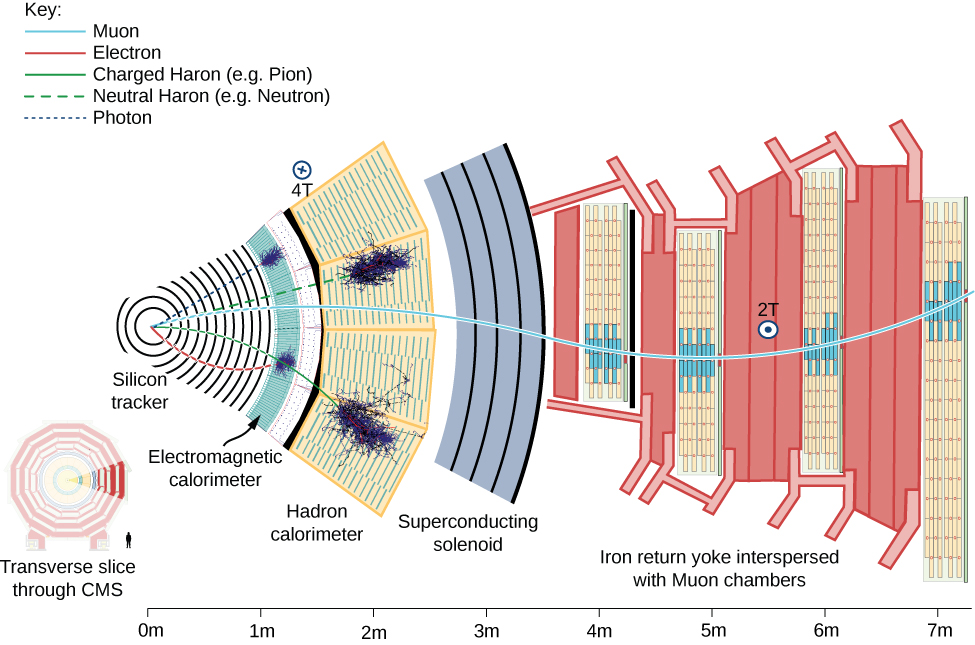
\includegraphics[width=12cm]{CMS.jpg}
    \label{fig:3}
\end{figure}
\par
Missing transverse energy, or MET, is another distinguishing attribute of electroweak interactions in hadron colliders. Let's focus only on a circular cross-section of our effectively cylindrical detector. Since the LHC collides proton beams with roughly the same energy, we expect that in the lab frame (the rest frame of the detector), we conserve energy and have 0 net momentum, in both the z-direction along the axis of the cylinder and in the ``transverse"  direction restricted to the plane of this cross-section. Now, let's suppose we measure tracks (i.e. charged particles that pass through the silicon tracker and the calorimeters) that are localized to a particular angular region ($\phi$) of the detector. If this momentum/energy is not canceled out by an equivalent signal that is 180$^{o}$ away within the circular cross-section, we seemingly have violated conservation of momentum in the transverse direction! We know that this is impossible, so we posit that momentum has indeed been carried by various particles in the opposite direction, and our detector has simply been unable to detect these ``invisible"  tracks. The MET is a single vector with direction and magnitude that cancels out the measured tracks in the detector, such that conservation of transverse energy/momentum is satisfied.
\par
MET is exceedingly important in any search for new physics. The presence of MET in a given event (a proton-proton collision in the case of the LHC) suggests that there may be some new particle that exists beyond the Standard Model. If there is little to no MET in a given event, then effectively everything has been accounted for, and there is little phase space available for a new signal. In experimental searches, a MET cut is often applied to reduce excessive Standard Model background. In CMS's inelastic dark matter searches, for example, a MET cut of 200 GeV is applied [11].
\par
Now, let's consider the two Feynman diagrams of interest in Figure~\ref{fig:2}. They both contain two LSPs that should not make a track in the detector and thus contribute to MET. In the top left diagram, the $\chi^{0}_{2}$ and the $\chi^{\pm}_{1}$ should have equal and opposite momentum. Then, according to existing SUSY searches, the most promising models involve a small mass splitting between the $\chi^{0}_{2}$ and the $\chi^{0}_{1}$ and the $\chi^{\pm}_{1}$ and the $\chi^{0}_{1}$. This means that the off-shell W$\pm$ and the Z carry off little momenta, and both LSPs have almost the same magnitude and direction of transverse energy/momentum as their parent particles. But, we've established that both SUSY parents travel in equal and opposite directions! As a result, the momenta of the LSP's effectively cancel out, and there is little net MET. As it stands, this signal would not pass the most straightforward cuts of a search.
\par
However, in a small fraction of events, a jet, or narrow cone of partons that occur after a quark or gluon hadronizes, is emitted from one of the protons before the decay proceeds [9]. As a result, the entire process, including both electroweakinos, is boosted with respect to the lab frame, after which the decay occurs as it would have otherwise. Since the $\chi^{0}_{2}$ and the $\chi^{\pm}_{1}$ are no longer back-to-back in the lab frame, neither are the LSPs! Therefore, the transverse vector sum of the LSP momenta is no longer zero, and depending on the momentum of the ISR jet and other kinematic properties of the particular event, the MET may pass the necessary cuts and lead to a meaningful signal.
\par
It is important to realize that within a given Feynman diagram, the expected signal can change depending on whether the electroweakinos are Higgsino-like of Wino/Bino-like. This is because Wino/Bino-like electroweakinos have different physical properties than Higgsino-like electroweakinos, and these differences lead to different kinematics for the expected decay products. Figure~\ref{fig:4} shows how the dilpeton mass distribution for a 20 GeV Z$_{*}$ changes depending on whether only kinematic phase space availability is considered (purple line) or if the electroweakinos are explicitly Higgsino-like (red) or Wino/Bino-like (blue) [9]. Clearly, the expectation of a search of inextricably dependent upon the composition of the mass eigenstates, and which weak eigenstates are assumed to contribute most to the mixing.
\begin{figure}[H]
    \centering
    \caption{} 
    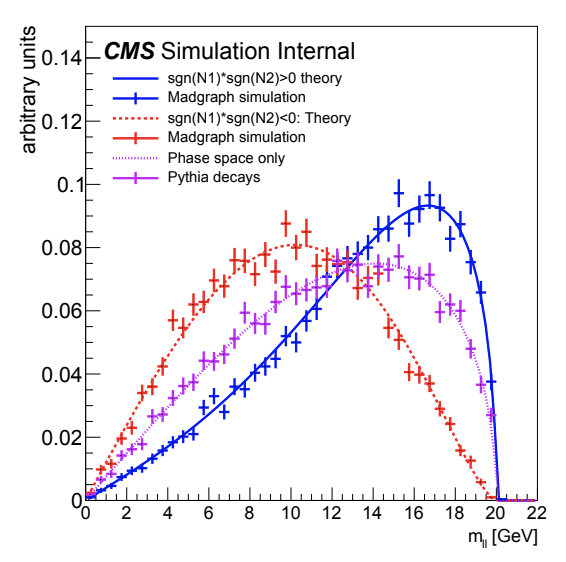
\includegraphics[width=6cm]{Dilepton.png}
    \label{fig:4}
\end{figure}
\par
The full procedure for identifying a signal from one of Figure~\ref{fig:2} Feynman diagrams is far more complex than has been described here, and cannot be reduced to simply identifying the desired dilepton kinematics and ensuring there exists sufficient MET to pass cuts. A plethora of other cuts must be applied, and even then, there still exists large backgrounds that provide a similar detector signature, such as QCD and other Z $\rightarrow$ $l\bar{l}$ decays [9]. Theorists have provided a list of cross-sections for SUSY processes with particular masses and mass splittings, and from a given cross-section and integrated luminosity of a detector, the number of expected SUSY events can be predicted before cuts. However, after applying cuts and requiring initial state radiation, etc, the number of events one would expect to find at a detector such as CMS is drastically reduced. Simulation tools can be a particularly useful way for experimentalists to predict the number of expected events for a given process before consulting physical data.

\subsection{Project Motivation and Signal Models}
Our goal was to simulate the two entirely electroweak SUSY processes from Figure~\ref{fig:2} at both generator and reconstruction level. We hoped to identify regions in which a distinctly SUSY signal can be discerned from Standard Model background, and investigate how this signal varies with the masses, mass splittings, and lifetimes of the electroweakinos. We hope that establishing of a signal region, with appropriately normalized distributions and proper attention to both the Higgsino and Wino/Bino mixing cases, will be helpful to other ongoing SUSY searches. Moreover, we applied relevant cuts, motivated both by the kinematics of the SUSY processes and the capabilities of the CMS detector, so that our computed events and cross-section are of a very similar scale to the number of events we would expect to detect at CMS. If CMS data fails to reveal a signal in the expected regions, perhaps particular SUSY models can be excluded, and if very few events survive our applied cuts, we may not be sensitive to particular models with existing technology. We denote left Feynman diagram from Figure~\ref{fig:2} as the "N2C1" case, while the right diagram, which lacks an intermediate Chargino in the bottom half the diagram, the "N2N1" case. Note that under MSSM, the N2N1 signal model cannot be produced in a Wino/Bino scenario. 
\par We planned to organize our the results from each sample into a grid, with the $\chi^{0}_{1}$ or $\chi^{0}_{2}$ mass and the mass splitting between the $\chi^{0}_{2}$ and the  $\chi^{0}_{1}$ on the two axes, and the signal cross section, or some other metric of the signal strength, in the grid itself.
\par
Our choice of signal models was motivated by prior work in the SUSY sector. Figure~\ref{fig:4} shows the results of various ATLAS searches for Electroweak SUSY signals [12]. The figure shows various mass combinations that can be excluded due to prior searches for prompt decays. However, since we simulated long-lived neutralinos and charginos, our samples covered a broad range of masses and mass-splittings, even if the corresponding location in figure~\ref{fig:4} had been previously excluded for prompt decays.
\begin{figure}[H]
    \centering
    \caption{} 
    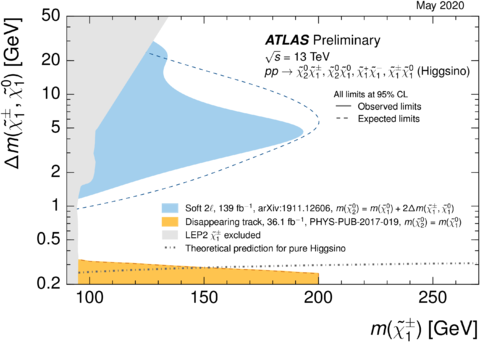
\includegraphics[width=12cm]{ATLAS.png}
    \label{fig:4}
\end{figure}
\par
Table 1 shows the mass configuration of the Higgsino-like samples we produced. We generated events corresponding with both the N2C1 and the N2N1 diagrams, and their corresponding production (i.e. hard process) cross-sections were found in [13, 14]. In the Higgsino scenario, the chargino mass always splits the mass of the two Neutralinos.
\begin{centering}
    \begin{table}[h]
        \begin{tabular}{||c|c|c|c|c|||}
             \hline $\chi^{0}_{2}$ Mass (GeV) & $\chi^{0}_{1}$ Mass (GeV) & N2C1 Cross Section (pb) & N2N1 Cross Section (pb)\\ [0.2ex]
             \hline
             110 & 100 & 4.295 & 2.726 \\
             \hline
             120 & 100 & 3.355 & 2.271 \\
             \hline
             130 & 100 & 2.663 & 1.905 \\
             \hline
             140 & 100 & 2.143 & 1.608 \\
             \hline
             135 & 125 & 2.009 & 1.220 \\
             \hline
             145 & 125 & 1.645 & 1.056 \\
             \hline
             155 & 125 & 1.360 & 0.918 \\
             \hline
             165 & 125 & 1.135 & 0.800 \\
             \hline
        \end{tabular}
        \caption{Higgsino-like Samples}
        \label{table:1}
    \end{table}
\end{centering}
\par
We produced samples with the following mass configurations for the Wino-Bino case (Table~\ref{table:2}). Since there is no N2N1 process in this scenario, the \textit{production} cross-section depends only on the $\chi^{0}_{2}$ and $\chi^{\pm}_{1}$ masses, which are identical in this model:
\begin{centering}
    \begin{table}[h]
        \begin{tabular}{||c|c|c||}
             \hline $\chi^{0}_{2}$ Mass (GeV) & $\chi^{0}_{1}$ Mass (GeV) & N2C1 Cross Section (pb) \\ 
             \hline
             125 & 120 & 10.034\\
             \hline
             125 & 115 & 10.034\\
             \hline
             125 & 105 & 10.034\\
             \hline
             125 & 95 & 10.034\\
             \hline
             125 & 85 & 10.034\\
             \hline
             150 & 145 & 5.1809\\
             \hline
             150 & 140 & 5.1809\\
             \hline
             150 & 130 & 5.1809\\
             \hline
             150 & 120 & 5.1809\\
             \hline
             150 & 110 & 5.1809\\
             \hline
        \end{tabular}
        \caption{Wino/Bino-like Samples}
        \label{table:2}
    \end{table}
\end{centering}
\par
For each mass configuration, we produced samples with a ctau of 1mm, 10mm, 100mm, and 1000mm. We also included an initial state jet of at least 80 GeV in our hard process. Note that although the shape of dilepton mass distribution varies depending on the whether the electroweakinos are Higgsino-like or Wino/Bino-like, we only took into account phase space availability, and used these different scenarios to motivate the chosen mass configurations.
\subsection{Sample Production and Generator-Level Cuts}
Figure~\ref{fig:5} steps through the various procedures required to produce both generator and reconstruction-level data for a given set of masses. 
\begin{figure}[H]
    \centering
    \caption{} 
    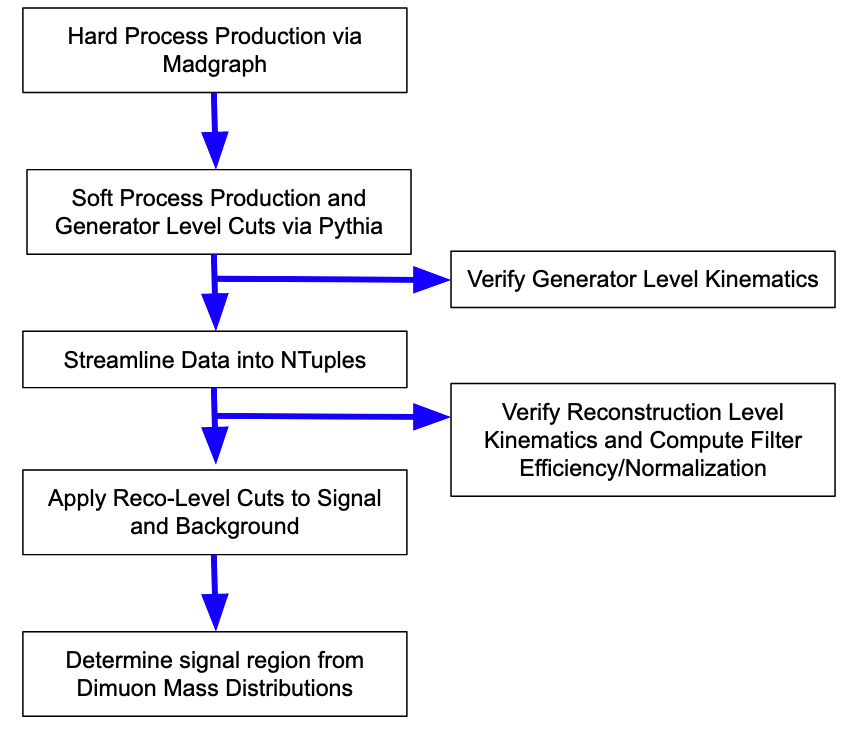
\includegraphics[width=12cm]{Workflow.png}
    \label{fig:5}
\end{figure}
\par
Before the final step, in which we apply a set of reconstruction-level cuts to our samples, it is necessary to compute the filter efficiencies and corresponding normalization factors from the prior steps. The reconstruction cutflows and corresponding plotting scripts require a conversion from the number of Monte Carlo events we produced to the number of true events that could be detected at the LHC over a given period of time. Therefore, we note of what percentage of events ``survive" the set of cuts at each step, and multiply the ``survival rate" at each step to compute a total filter efficiency. We consult Table~\ref{table:1} to determine the cross-section of a given process for proton-proton collisions, and scale this value down as we apply various restrictions to our event generation.
\subsubsection{Hard Process Generation in Madgraph}
Madgraph is commonly used by CMS to simulate processes in particle colliders such as the LHC. In particular, Madgraph is well-equipped for matrix element generation, or the production of a given process to lowest order with no additional hadronization or parton showering. Therefore, we used Madgraph solely to produce p p $\rightarrow$ $\chi^{0}_{2}$ $\chi^{\pm}_{1}$  or p p $\rightarrow$ $\chi^{0}_{2}$ $\chi^{0}_{1}$. We initially attempted to decay our electroweakinos and compute the process to a higher order in Madgraph, but found it was not sensitive to small resonance widths for our $\chi^{0}_{2}$  and $\chi^{\pm}_{1}$. Since the width scales inversely with the particle lifetime, this inhibited us from exploring long-lived scenarios. We used Madgraph5, the most recent version of the program, throughout this study, and ran Madgraph on CERN's LXPLUS machine. Although Madgraph's output can be organized into human-readable ``.lhe" files, we used Madgraph to produce a gridpack. A gridpack is a file of Madgraph code that provides a framework for event generation at a larger scale. Once we produced our gridpacks, we were able to generate our leading-order diagram in Madgraph alongside higher-order showerings in Pythia, effectively combining two steps into one.
\par
We defined our hard process using SLHA template cards, which we used as input for gridpack generation. We used a ``proc" card that defines the constituents of the hard process we intend to simulate, a ``run" card that sets various conditions that all events must satisfy, and a ``customize" card that sets the masses of our electroweakinos. Figure~\ref{fig:6} shows a given run card for an N2C1 sample with initial state radiation.
\begin{figure}[H]
    \centering
    \caption{Example Proc Card} 
    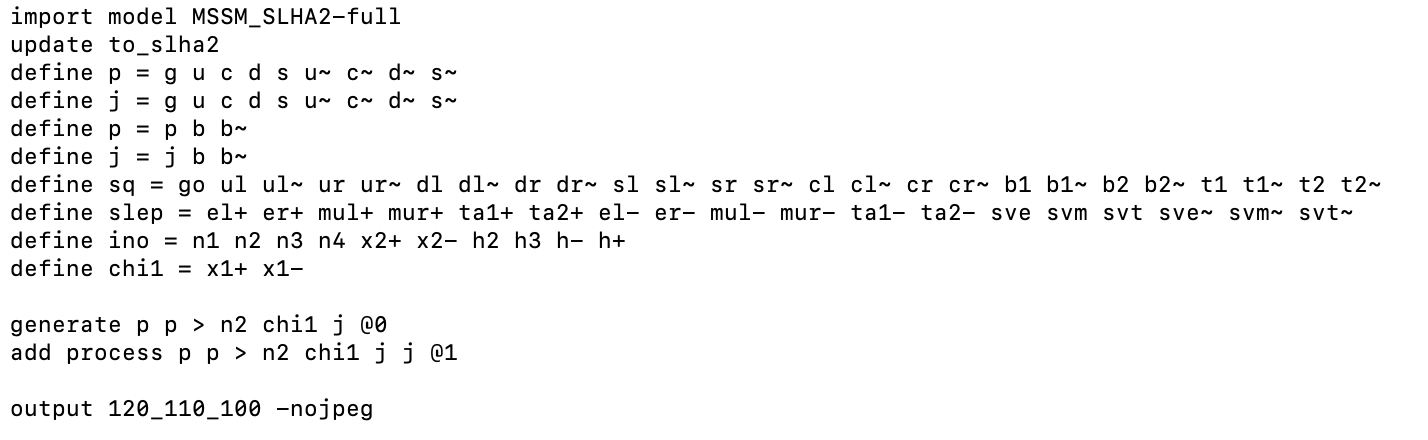
\includegraphics[width=12cm]{Proc_Card.png}
    \label{fig:6}
\end{figure}
\par
In the sample generated from the proc card shown in Figure~\ref{fig:6}, the primary process we generated required one initial state jet, denoted ``j". However, we also included higher order events with two initial state jets, as these processes do occur in collisions, and can be kinematically favorable to signal sensitivity. The zeroth and first order of the given process are denoted by ``@0" and ``@1" respectively in the card. However, the rate at which initial state radiation occurs is an important consideration when determining a total filter efficiency. We produced ISR inclusive samples as well, for which the lowest order process had 0 initial state jets. Madgraph outputs a total cross-section associated with each generated sample during gridpack generation. We took $\frac{\text{ISR Cross Section}}{\text{ISR inclusive Cross Section}}$ to determine the rate of ISR production, and included this factor in our computation of the filter efficiency. Therefore, for a given set of masses in the Higgsino case, we produced four gridpacks: one for the N2C1 ISR case, the N2C1 ISR inclusive case, the N2N1 ISR case, and the N2N1 ISR inclusive case. The production of the four gridpacks takes about half a day. For the Wino/Bino scenario, only two gridpacks were required for a given $\chi^{0}_{2}$ mass, since the $\chi^{\pm}_{1}$ always had the same mass as the $\chi^{0}_{2}$ and there is no parallel N2N1 process.
\par
For our run card, we used almost entirely the same configurations as the CMS SUSY group at [11]. Most notably, we only generate events with an initial state jet of at least 80 GeV in the ISR case, while this requirement is not in place for ISR inclusive samples.
\subsubsection{Soft Process Production in Pythia}
After producing the Madgraph gridpack, we used the same script to both generate the hard process in Madgraph and decay the electroweakinos in Pythia. It was not necessary to produce a precise number of generator-level events, as our distributions would be normalized relative to our effective total cross section at later steps. However, we wanted to produce enough events so that we could assess generator-level kinematics with high statistical confidence, yet ensure that event production would not be too computationally taxing. We attempted to produce 100,000 events for a given sample. To maintain computational efficiency, we used LXPLUS's condor batch system to separate this computation into 200 jobs with 500 events each, running in parallel. A given job produces an AOD root file for each ctau. The AOD contains the generator and reconstruction-level information for the set of events.
\par
Once the hard process electroweakinos and initial state jet are produced in Madgraph, Pythia computes the following independently for each lifetime before outputting the AOD:
\begin{enumerate}
    \item Hadronization and Parton Showering
    \item Jet Matching
    \item Implementation of Generator-Level User Cuts
\end{enumerate}
\par
We used CMS's Pythia8 Hadronizer Filter to process the particles provided by Madgraph. This procedure provides a complete list of partons for a given event, known as the Pythia event listing. Again, we required the Z-boson to decay to a muon pair, as muons are by far the easiest Z-decay to reconstruct in the detector. The Z$\rightarrow$ $\mu^{+}\mu^{-}$ branching ratio (approximately 3.6\%) is incorporated into our overall filter efficiency. However, Madgraph and Pythia both produce the expected number of jets, but each jet from Madgraph must be matched with a jet from Pythia, otherwise too many jets are produced in total [15]. Since Madgraph is better equipped for producing harder particles, while Pythia is better with soft particles, we set parameters for Madgraph and Pythia independently (known as the XQCUT and QCUT respectively) that prevent jet production that doesn't satisfy a constraint on a particular kinematic attribute known as the kT. [15] should be consulted for a concise explanation of the XQCUT, QCUT, and kT. We set the XQCUT to 30 and the QCUT to 25. In short, the XQCUT and QCUT allow us to discard events with a problematic interface between Madgraph and Pythia with respect to jet production. We usually lose over half of our events due to matching parameters, even before applying user cuts.
\par
Figure~\ref{fig:7} shows the full set of configurations used for hadronzation/parton showering and jet matching in Pythia.
\begin{figure}[H]
    \centering
    \caption{Pythia Configuration} 
    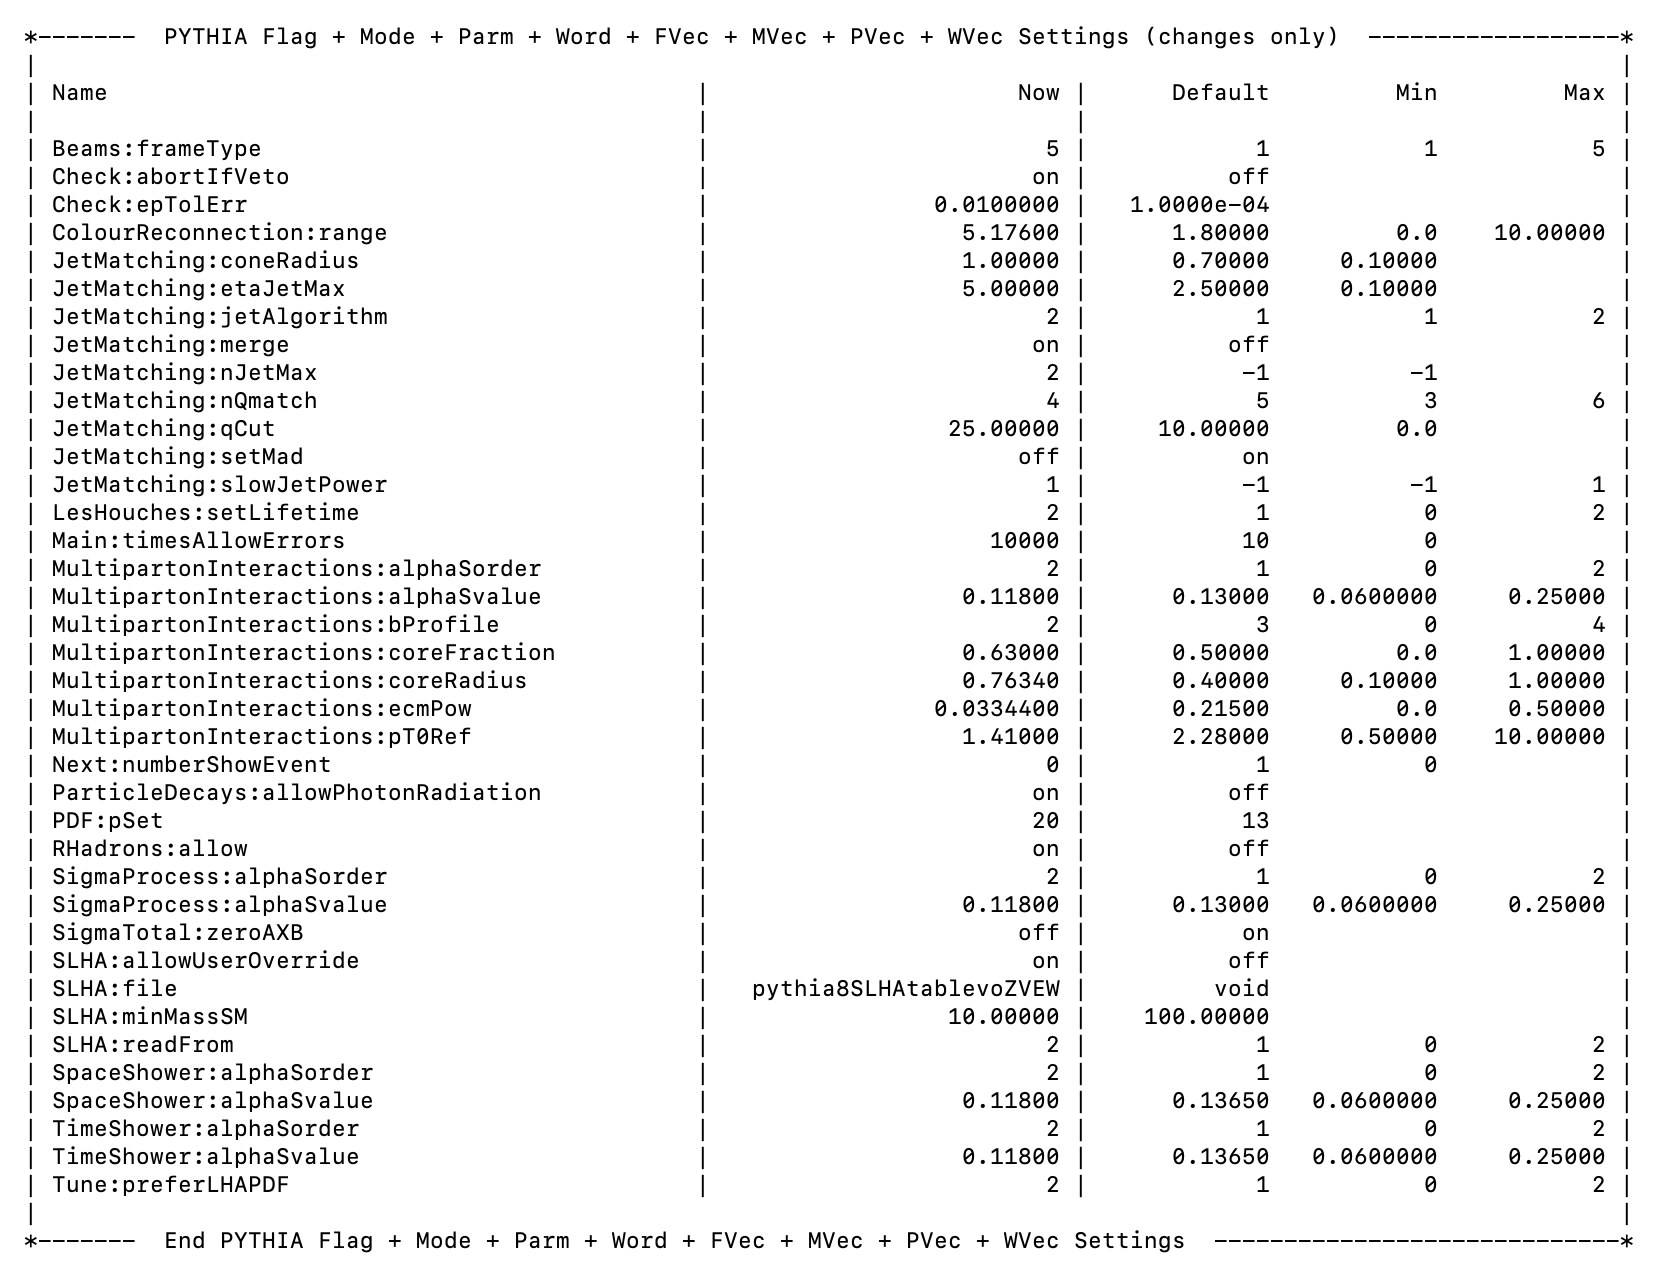
\includegraphics[width=12cm]{PythiaConfigs.png}
    \label{fig:7}
\end{figure}
\par
Lastly, we specify a set of additional cuts at generator-level. Although we later apply a set of reconstruction-level cuts that ensure that our final events are measurable at CMS, we would like our generator-level kinematics to be correspond closely with those of the final events during kinematic verification of generator-level properties. As a result, we discard events that lack an 80 GeV initial state jet and that do not include at least 80 GeV of MET. After considering matching and applying these generator level cuts, usually only about 30,000 of the 100,000 attempted events reach the output AODs in N2C1 processes, and only about 16,000 out of 100,000 events in N2N1 processes (these values vary slightly with the mass configuration and lifetime).
\subsection{Creation of NTuples and Computation of New Effective Cross-Section}
As specified in the previous section, all relevant data is stored in a set of AOD root files. Since each job produces 4 AODs (one for each lifetime), we are left with 800 AODs that together contain the data associated with a particular mass configuration. Moreover, these files are rather large, so it is necessary to consolidate the data in a more efficient manner (though we do iterate through the relevant AODs when analyzing generator-level kinematics).  Moreover, CMS's inelastic dark matter (IDM) analysis group, whose reconstruction-level cuts we later borrow, requires data to be in an NTuple format in order for their existing code to work. Fortunately, the IDM group also provides the necessary code to convert a set of AOD files to an NTuple. Using this framework, we were able to repackage our data into 4 NTuple root files, one for each ctau. Note that we maintained separate NTuples for the N2C1 and N2N1 processes, and that no additional cuts are applied in our conversion from AODs to NTuples.
\par
An NTuple is effectively a tree structure, with branches that correspond to particular generator-level or reconstruction-level data categories, such as MET, muon pT, or number of jets. Each leaf on the branch corresponds to the data associated with a particular event. Therefore, the total number of entries/leaves corresponds to the sum of the events originally from the AODs. Therefore, the Pythia contribution to the total filter efficiency, due both to matching and user-implemented cuts, equals $\frac{\text{Events in NTuple}}{\text{Events Attempted}}$, where our attempted events was usually 100,000. Let's denote our effective process cross-section, after considering our generator and computational cuts, as $\sigma_{g}$, and our initial theoretical production cross-section as $\sigma_{T}$. Let $\epsilon_{g}$ denote the total filter efficiency after event production. Then, the following holds:
\[\sigma_{g} = (\epsilon_{g})(\sigma_{T})\]
where
\[\epsilon_{g} = (\text{Madgraph Efficiency})*(\text{Pythia Efficiency})*(Z\rightarrow \mu^{+}\mu^{-} \text{branching ratio})\]
From prior sections, we recall:
\begin{centering}
    \begin{table}[h]
        \begin{tabular}{||c|c|c||}
        \hline Madgraph Efficiency & Pythia Efficiency & $Z\rightarrow \mu^{+}\mu^{-}$ branching ratio \\
        \hline
        $\frac{\text{ISR Cross Section}}{\text{ISR inclusive Cross Section}}$ & $\frac{\text{Events in NTuple}}{\text{Events Attempted}}$ & 0.0366 \\
        \hline
        \end{tabular}
        \label{table:3}
        \caption{Generator-Level Efficiency Contributions}
    \end{table}
\end{centering}
\par
Note that $\epsilon_{g}$ does not vary significantly with different mass configurations or lifetimes, though as stated before, the Pythia efficiency in N2N1 samples tends to be half of the N2C1 samples. The $Z\rightarrow \mu^{+}\mu^{-}$ branching ratio is the greatest contributor to signal suppression, and it is difficult to circumvent this inefficiency without more reliable electron and hadron ID at CMS.
\par
From our new process cross-section, we can normalize our generated events (the number of entries in the NTuple) to a luminosity-dependent ``real" events. This normalization factor, which we denote \textit{N} is given by:
\[N = \frac{\text{(Run Luminosity)}(\sigma_{g})}{(\text{Events in NTuple})}\]
We verified reconstruction-level kinematics, muon reconstruction, and other relevant metrics using NTuple-formatted data. Relevant figures are included in the Reconstruction-Level Kinematics Section.
\subsection{Reconstruction-Level Cuts}
Thus far in our sample generation procedure, we have applied cuts based entirely on generator-level computations by considering jet momentum, missing energy, etc \textit{before} considering how the partons themselves interact with the detectors, i.e. our reconstruction-level data. Since we have produced our reconstruction-level data, it is advisable to apply an additional set of cuts more directly informed by the limitations of the CMS detector and the distinct signature we expect to see from this type of physical process.
\par
We chose to use a set of the IDM group's reconstruction-level cuts as our final filter. The choice was a matter of convenience, but was also physically motivated. Figure~\ref{fig:8} shows a benchmark model for inelastic dark matter searches [17]. Both this process and our electroweak SUSY processes of interest rely on ISR and a missing energy trigger, as well as soft lepton decays from an off-shell intermediate particle, resulting in definitive kinematic endpoints in both cases. It is presumptuous to conclude that neutralinos and charginos constitute the dark matter candidates, and that Figure~\ref{fig:8} is in fact equivalent to our SUSY Feynman diagrams. However, the similarities are striking, and the use of the IDM's group's cuts is strongly motivated.
\begin{figure}[H]
    \centering
    \caption{IDM Feynman Diagram} 
    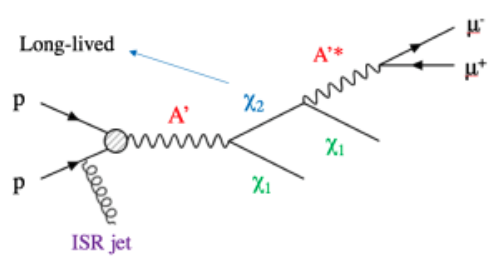
\includegraphics[width=12cm]{iDM.png}
    \label{fig:8}
\end{figure}
\par
The following lists the inclusive reconstruction-level cuts in the order they are applied [17].
    \begin{enumerate}
        \item No Cuts
        \item HEM Veto
        \item Trigger fired (120 GeV MET No Muons)
        \item MET $>$ 200 GeV
        \item $|\text{CaloMET - PFMET}|$/CaloMET $<$ 1
        \item nJets $>$ 0 (pT $>$ 30 GeV)
        \item Leading Jet Eta $<$ 2.4
        \item Leading jet pT $>$ 80 GeV
        \item $|\text{DeltaPhi(MET, leading jet)}|$ $>$ 0.5
        \item $|\text{DeltaPhi(MET, all jets)}|$ $>$ 0.5
        \item nJets $<$ 3 (pT $>$ 30 GeV)
        \item 0 b-tagged jets
        \item Good dSA Muons $>=$ 1
        \item Good dSA Muons $>=$ 2
        \item Two Best dSA Muons (dSA 0 and dSA 1) are different
        \item Cosmic Veto (min(cosalpha $>$ -0.94))
        \item Good dSA-dSA vertex
        \item Best dSA 0 pT resolution $<$ 1
        \item Best dSA 1 pT resolution $<$ 1
        \item Vertex $\chi^{2}$ $<$ 4
        \item MT $<$ 200 GeV
        \item M$_{\mu\mu}$ $<$ 30 GeV
        \item dR(muons) $<$ 0.9
        \item dSA 0 and dSA 1 have opposite charge
        \item Selected muon 0 dxy $>$ 0.1 cm
        \item Selected muon 1 dxy $>$ 0.1 cm
    \end{enumerate}
\par
After applying these cuts, we separate the remaining events into three binning regions:
    \begin{enumerate}
        \item 0 GM-dSA matched
        \item 1 GM-dSA matched
        \item 2 GM-dSA matched
    \end{enumerate}
\par
A global muon (GM) muon is one that registers a track in CMS's  inner tracker. The inner tracker is particularly well-suited for measuring the magnitude and direction of a particle's momentum, and generally has better resolution than the calorimeters and other constituents of the detector. At higher ctaus, many $\chi^{2}_{0}$s don't decay until after passing through the inner tracker, which has radius of about 1 meter. Displaced standalone muons (dSA) are detected in the outer muon chambers, but do not necessarily leave a track in the inner tracker. Therefore, our post-cut binning is based on how well we can interface the muon tracks in the inner tracker with stopped muons in the muon chamber. The 2 GM-dSA matched muons bin is therefore expected to have the least events, but the reconstruction of these events is especially trustworthy. 
\par
As a last step in data processing, we iterate through the aforementioned reconstruction-level cuts and ignore events in our signal nTuples that do not satisfy these cuts, using the IDM group's existing analysis code written in C++. For the Higgsino scenario, we keep the N2C1 and N2N1 cases separate, so the relevant cross-sections and normalization factors are specific to a given mass configuration/hard process combination. The remaining events can be plotted, their cross-section can be measured, etc, and various signal regions can be identified. Therefore, we acquire a reconstruction-level filter efficiency  $\epsilon_{r}$ as well due to the application of cuts, which can be computed as the percent of remaining events surviving after the application of each cut. Therefore, our final process cross-section $\sigma_{r}$ after the application of all cuts can be expressed as:
\[\sigma_{r} = (\epsilon_{g})(\epsilon_{r})(\sigma_{T})\]
The final normalization factor from an event in our nTuple to a measurable, reconstructed event we expect to see at CMS is given by:
\[N = \frac{\text{(Run Luminosity)}(\sigma_{r})}{(\text{Events in NTuple})}\]
\par
At this step, we also consider Standard Model Monte Carlo (MC) background, and apply the same set of cuts to the background data that was taken during a given run of the LHC (we chose 2018 Run 2). The following process constitute the SM background considered by the IDM group:
\begin{enumerate}
    \item QCD
    \item Z $\rightarrow$ ll + jets
    \item Z $\rightarrow$ $\nu\nu$ + jets
    \item W $\rightarrow$ l$\nu$ + jets
    \item Top Quarks
\end{enumerate}
\subsection{Verification of Generator-Level Kinematics}
It is essential to ensure that the samples we've generated represent the particular physical process we are trying to model, as opposed to immediately searching for a promising signal region and comparing with background. Therefore, after generating our hard process in Madgraph and decaying our particle in Pythia, we histogrammed various observables that define the important features of our electroweak diagram and ensured that our generator-level kinematics matched expectations.
\par
We histogrammed a wide variety of generator-level attributes, as shown in Figure~\ref{fig:9}. I'll only include a few of the more essential plots here, shown in Figure~\ref{fig:9}. These figures were produced using data from the Higgsino-like N2C1 sample with a $\chi_{2}^{0}$ mass of 110 GeV with a ctau of 1 mm and a $\chi_{1}^{0}$ mass of 100 GeV, though similar plots with analogous results were produced for different mass configurations. Note that these plots are not normalized, so the number of entries in a bin does not reflect the number of events expected to be detected at CMS.
\par
\begin{figure} [H]
\begin{subfigure}{.5\textwidth}
  \centering
  % include first image
  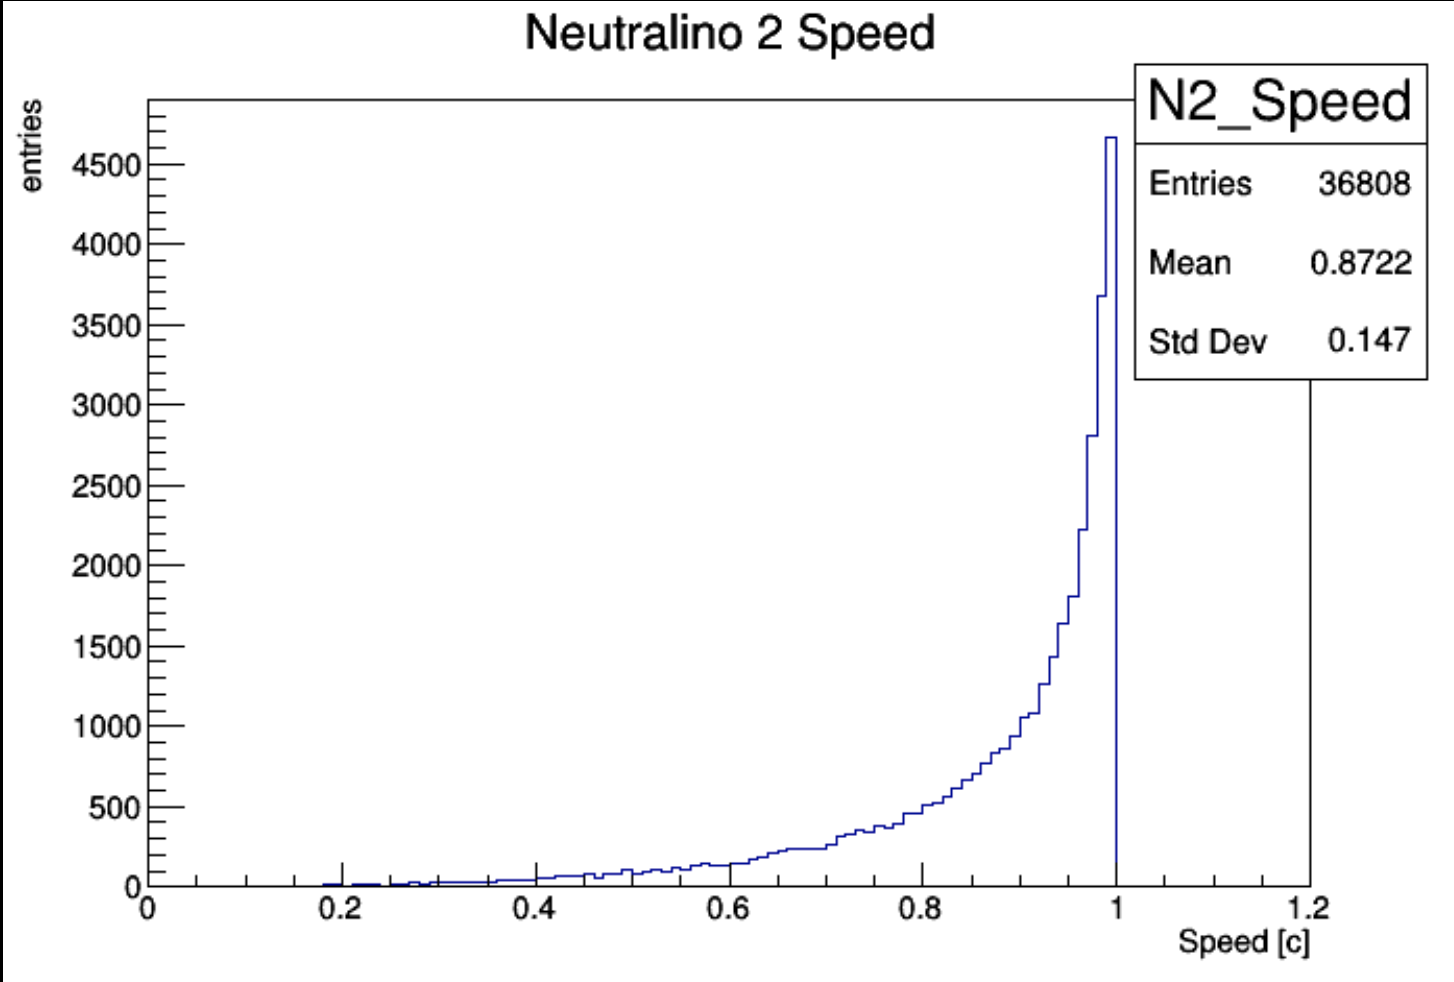
\includegraphics[width=.8\linewidth]{ZBeta.png}  
  \caption{$\chi_{2}^{0}$ Speed}
  \label{fig:sub-first}
\end{subfigure}
\begin{subfigure}{.5\textwidth}
  \centering
  % include second image
  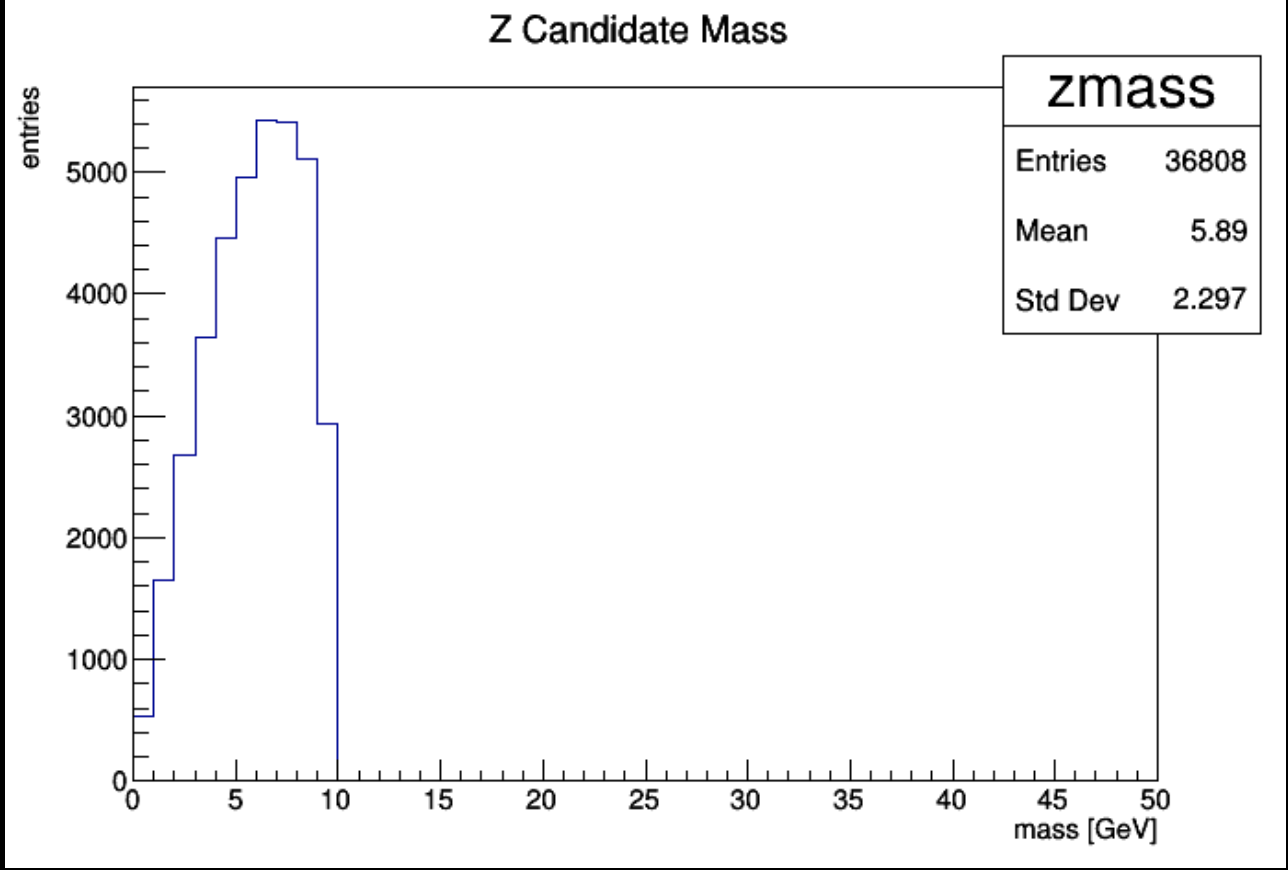
\includegraphics[width=.8\linewidth]{ZMass.png}  
  \caption{Z Candidate Mass}
  \label{fig:sub-second}
\end{subfigure}
\begin{subfigure}{.5\textwidth}
  \centering
  % include third image
  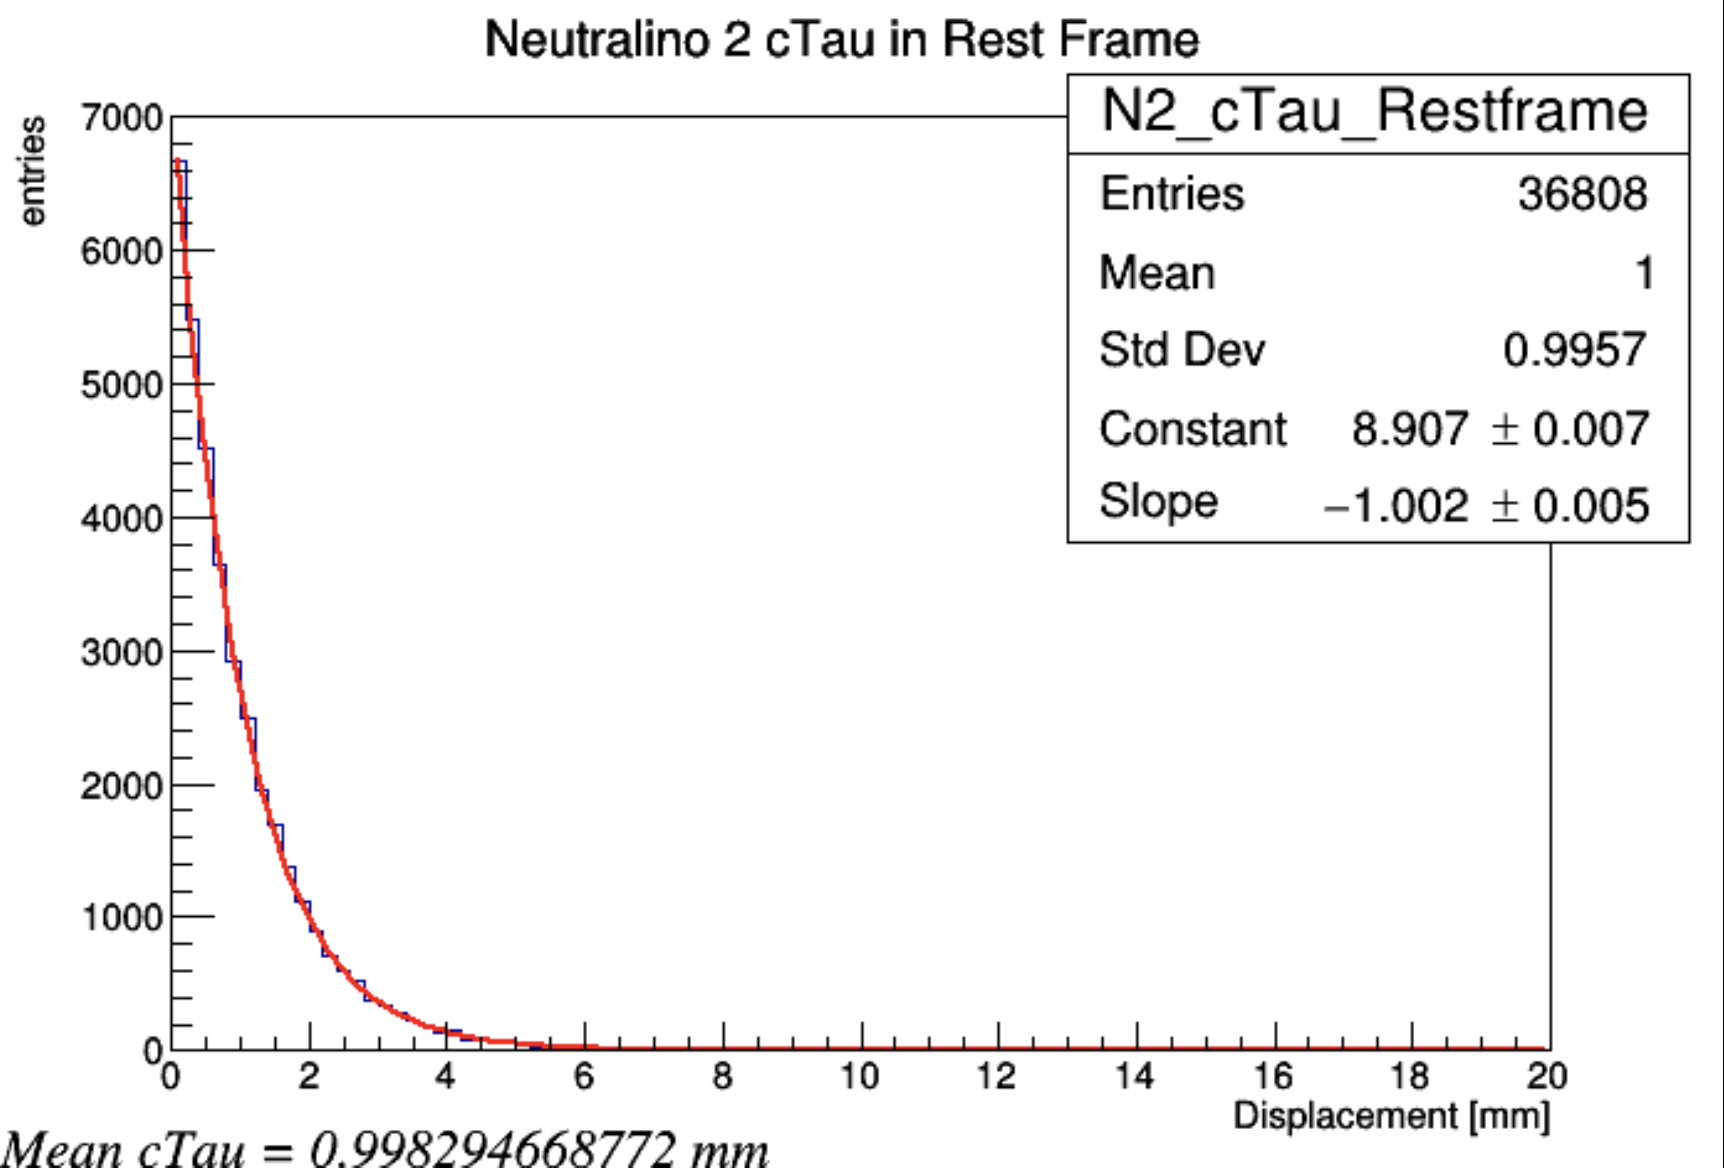
\includegraphics[width=.8\linewidth]{ctau.png}  
  \caption{$\chi_{2}^{0}$ ctau}
  \label{fig:sub-third}
\end{subfigure}
\begin{subfigure}{.5\textwidth}
  \centering
  % include fourth image
  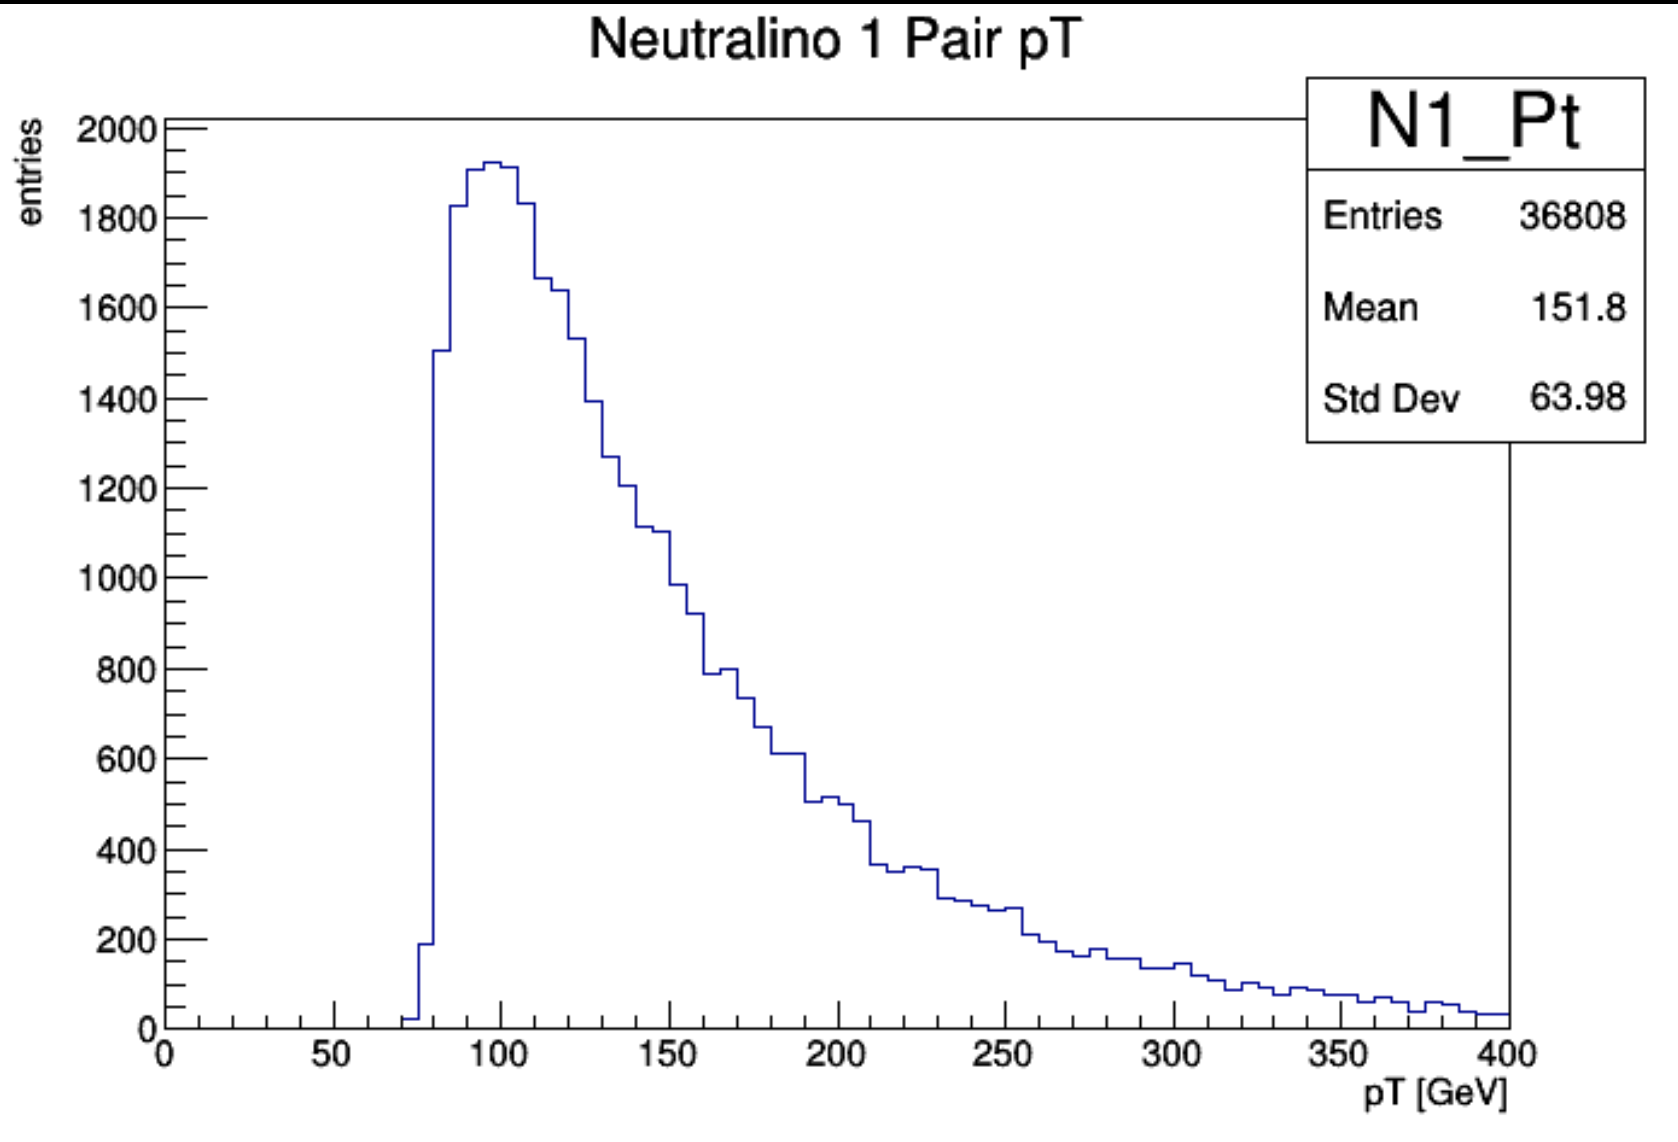
\includegraphics[width=.8\linewidth]{N1pT.png}  
  \caption{$\chi_{1}^{0}$ Pair 4-vector Sum}
  \label{fig:sub-fourth}
\end{subfigure}
\caption{Kinematic Verification at Generator-Level}
\label{fig:9}
\end{figure}
Figure~\ref{fig:sub-first} shows that our relativistic calculations of the $\chi_{2}^{0}$ obey the kinematic limit that the particle cannot move faster than c, though oftentimes it travels very close to the speed of light. This also ensures that the ctau, the speed of light times the mean lifetime of the particle, is an appropriate metric of the average decay length of the $\chi_{2}^{0}$, though the presence of a tail of slower $\chi_{2}^{0}$s indicates that the decay length may be substantially shorter than the ctau for a small subsets of events. Figure~\ref{fig:sub-second} shows that the kinematics of Z-candidate, which consists of the 4-vector sum of the Muon decay products, is consistent with the $\chi_{2}^{0}$ - $\chi_{1}^{0}$ mass splitting (10 GeV in this particular sample). This verifies that the observation of two soft, displaced muons could indicate the possibility of an electroweak SUSY process with a compressed mass spectrum, the discerning feature in our signal model. Figure~\ref{fig:sub-third} illustrates that we properly simulate the cTau, as the mean displacement of the $\chi_{2}^{0}$ is very nearly the expected value of 1 mm (again, we don't expect exact precision because the $\chi_{2}^{0}$ cannot move at the speed of light). Moreover, the histogram is well-fitted by an exponential decay function, the typical model for particle decays. Figure~\ref{fig:sub-fourth} shows the transverse momentum of the sum of the $\chi_{1}^{0}$ LSPs. We expect there to be a kinematic edge at 80 GeV, because we apply the $>$ 80 GeV generator-level MET cut, and the LSPs are the source of the MET (note that when the $\chi_{2}^{0}$ ctau is on the same order as the inner tracker, the $\chi_{2}^{0}$ will contribute to the MET, though for ctau = 1 mm this should not be the case). There is a small tail in the distribution with pT $<$ 80 GeV, which suggests perhaps a slight inaccuracy at generator-level, or perhaps a source of uncertainty that allows for a few event to pass the cuts with MET $<$ 80 GeV. However, this portion of the distribution was rather small, so we concluded that generator-level production worked largely as expected.
\subsection{Verification of Reconstruction-Level Kinematics}
\subsubsection{Gen-Reco Muon Matching}
Since we had reaffirmed that the correct process was being produced at generator level, the next logical step was to verify that Pythia was adequately reconstructing our tracks, particularly our muons, so that we could trust that an analysis of reconstruction-level data reflected the generator-level phenomena we were interested in. Using our nTuples, which contain both generator-level and reconstruction-level data, we matched our ``gen" muons with our best guess for the corresponding ``reco" muons. After matching, we compared the kinematics of the gen level pair with the kinematics of the reco-level pair - a rough estimate of the effectiveness of reconstruction can be garnered by comparing the kinematics of the pairs after this back of the envelope matching. It was rare to have more gen muons than reco muons in a given event, as there were many additional tracks that passed muon ID at reco-level, within jets and other features of the events. Figure~\ref{fig:10} shows the distributions for the number of gen level muons per events and the number of reco level global muons per event. In this section, all plots come from the N2N1 sample with a $\chi_{2}^{0}$ mass of 130 GeV and ctau of 1mm, and a $\chi_{1}^{0}$ mass of 100 GeV.
\par
\begin{figure} [H]
\begin{subfigure}{.5\textwidth}
  \centering
  % include first image
  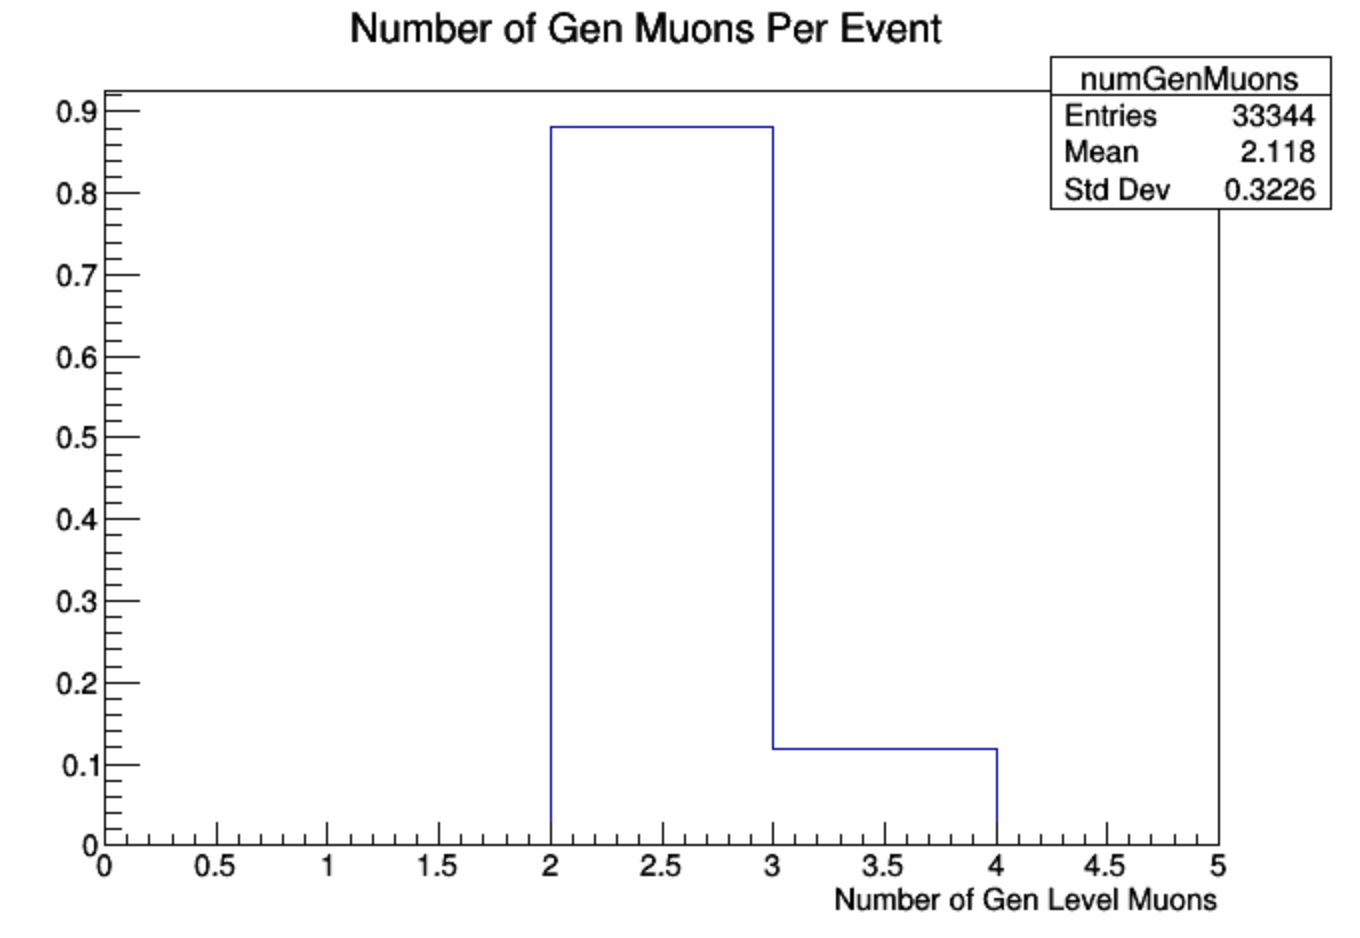
\includegraphics[width=.8\linewidth]{GenMuons.png}  
  \caption{Number of Gen Muons Per Event}
  \label{fig:sub-first2}
\end{subfigure}
\begin{subfigure}{.5\textwidth}
  \centering
  % include second image
  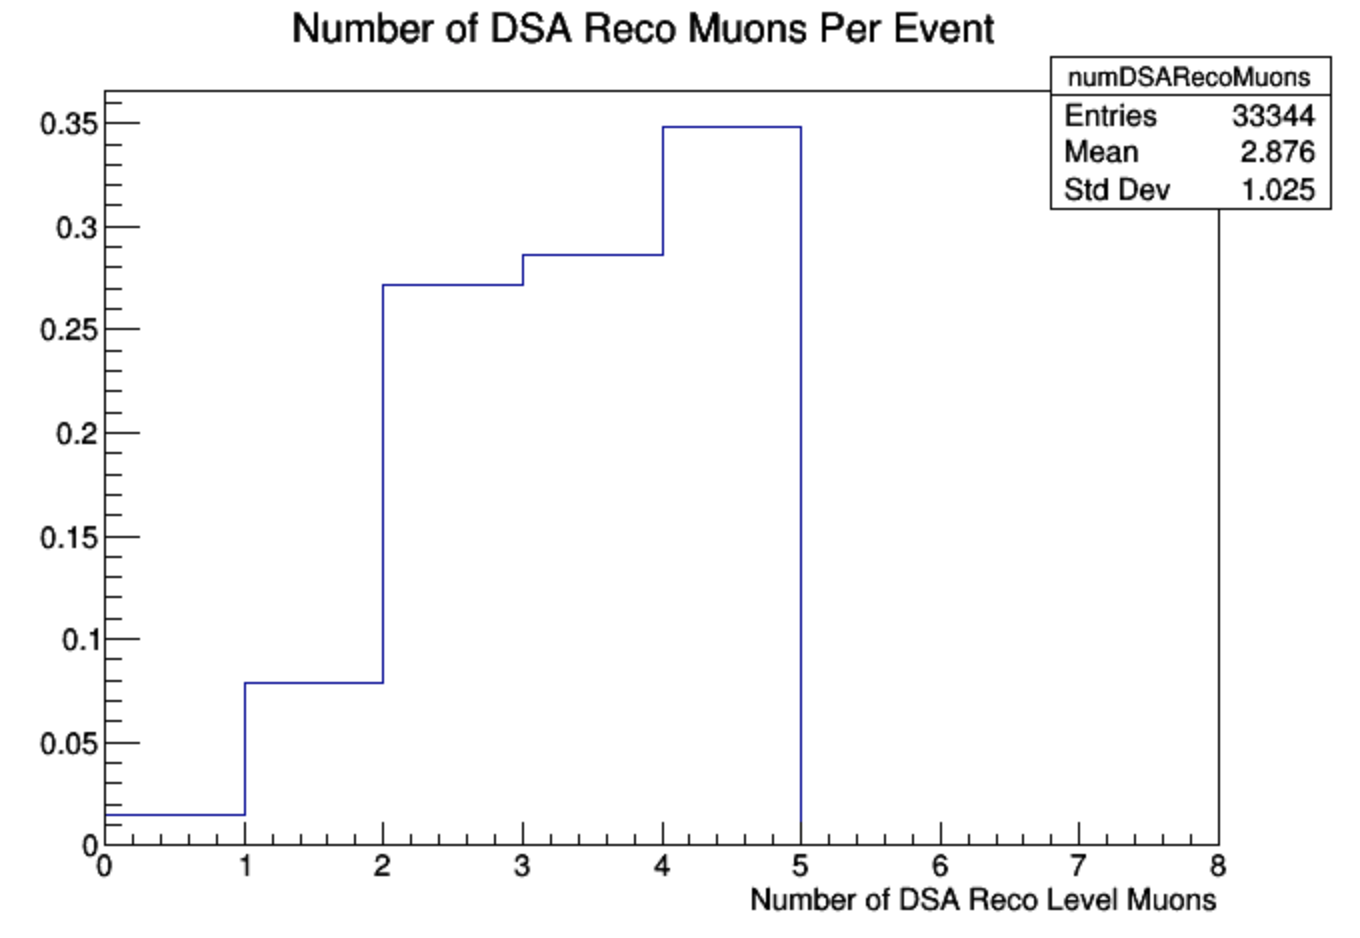
\includegraphics[width=.8\linewidth]{DSAMuons.png}  
  \caption{Number of DSA Reco Muons Per Event}
  \label{fig:sub-second2}
\end{subfigure}
\caption{Muons per Events Distributions}
\label{fig:10}
\end{figure}
\par
It is important to note that at gen-level, we almost always have only two muons, both from the off-shell Z decay. The presence of the third muon occurs when the off-shell W boson, the decay product of a $\chi_{1}^{\pm}$, decays leptonically instead of into quarks. Note that leptons from the W boson tend to be softer than those from the Z.
\par
We matched our gen muons to both dSA muons and global muons separately. Since global muons are detected by the inner tracker, their measured kinematics are generally more consistent with gen muons, but it is possible that the muon did not leave a track, and thus is only present in the dSA collection. Our straightforward matching algorithm was as follows:
\begin{enumerate}
    \item Separate gen-level and reco-level muons by charge
    \item Order gen muons in order of decreasing pT
    \item Starting with highest pT gen muon, iterate through reco muons of the same charge, and match with muon for which $\Delta$R(gen, reco) is the smallest
\end{enumerate}
\par
We order the gen muons by pT because the harder muons are more likely to be a component of the dimuon signal necessary to reconstruct the off-shell Z. $\Delta$R measures the angular distance between two 4-vectors, serving as a metric for kinematic similarity. It is defined as:
\[\Delta R = \sqrt{(\Delta\eta^{2})+(\Delta\phi^{2})}\]
Figure~\ref{fig:11} shows the distribution of $\Delta$R values between matched gen muons and dSA reco muons. For all matches, $\Delta$R is especially small, which suggests that our matching has been largely effective, and the gen muons were well-reconstructed by Pythia. This figure also suggests that matching gen muons with dSA muons is an accurate procedure, and any loss in resolution for the muons that don't leave an inner track can largely be ignored.
\begin{figure}[H]
    \centering
    \caption{$\Delta$R Distribution from Gen-Reco Muon Matching} 
    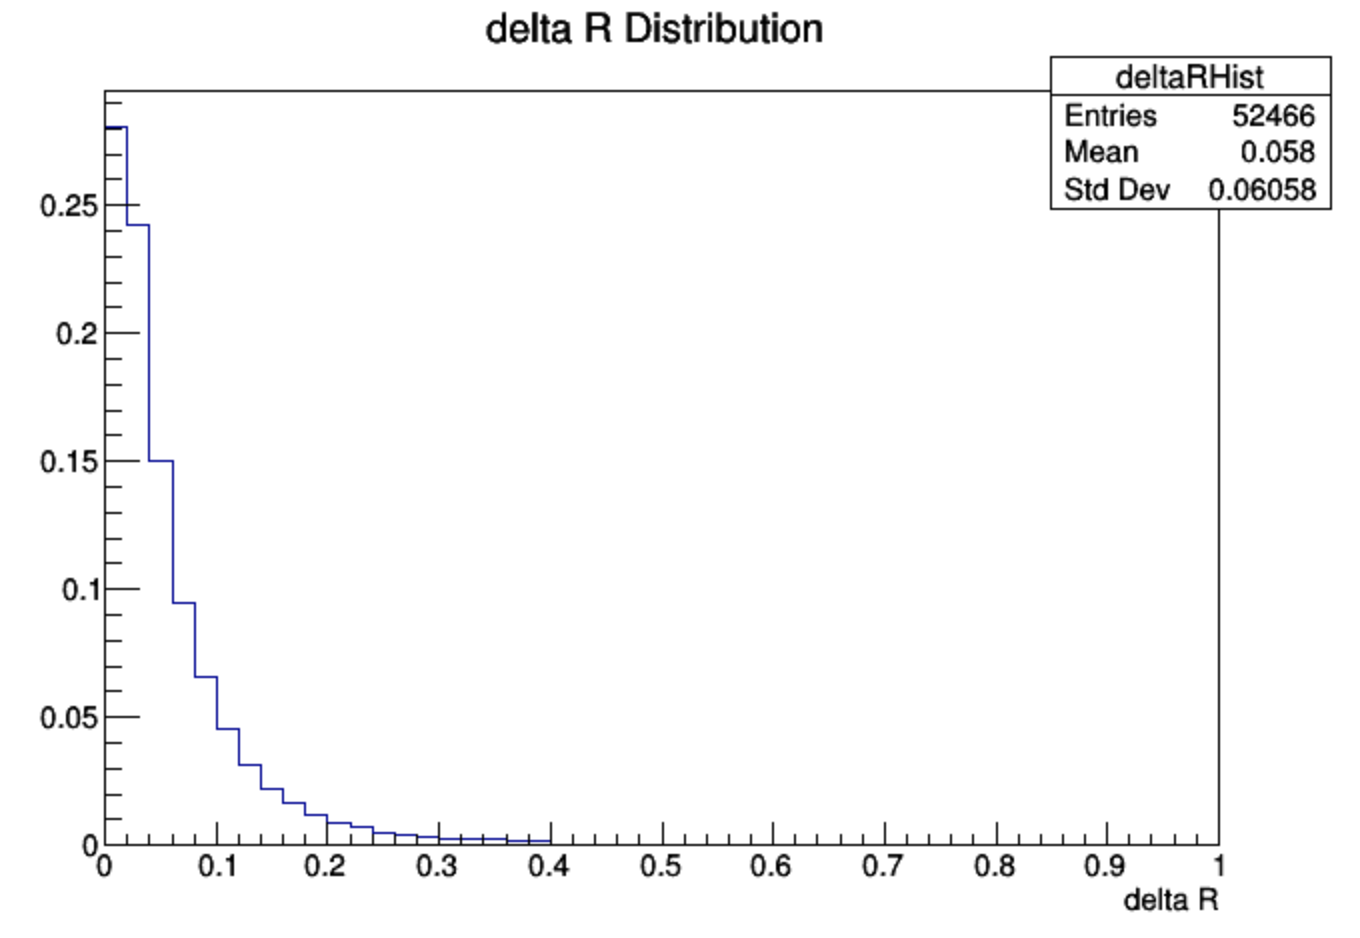
\includegraphics[width=12cm]{deltaR.png}
    \label{fig:11}
\end{figure}
\par
Next, we can directly compare the kinematics of gen muons and their matched reco muons. Figure~\ref{fig:12} is a 2D histogram that compares the generator-level and reconstruction-level pT of matched muons. In a scenario with perfect matching, all entries in the histogram will fall within bins along the diagonal, for which the two pTs match identically. However, as is clear from the figure, there exists some uncertainty and reconstruction inaccuracy, which can greatly overestimate or underestimate the pT of the reco-level muon. Figure~\ref{fig:11} both establishes that our somewhat simplistic matching algorithm is effective, and that the angular position of the reconstructed muons is very similar to their generator-level counterparts. Therefore, the "noise" in the histogram can be attributed to inaccuracies in pT reconstruction, as opposed to an issue regarding matching itself. As with the our other distributions, the data has not been normalized, so the values in the bins themselves do not reflect the number of detectable events during a given run of the LHC.
\begin{figure}[H]
    \centering
    \caption{Distribution of Gen pT/reco pT in Matched Muons} 
    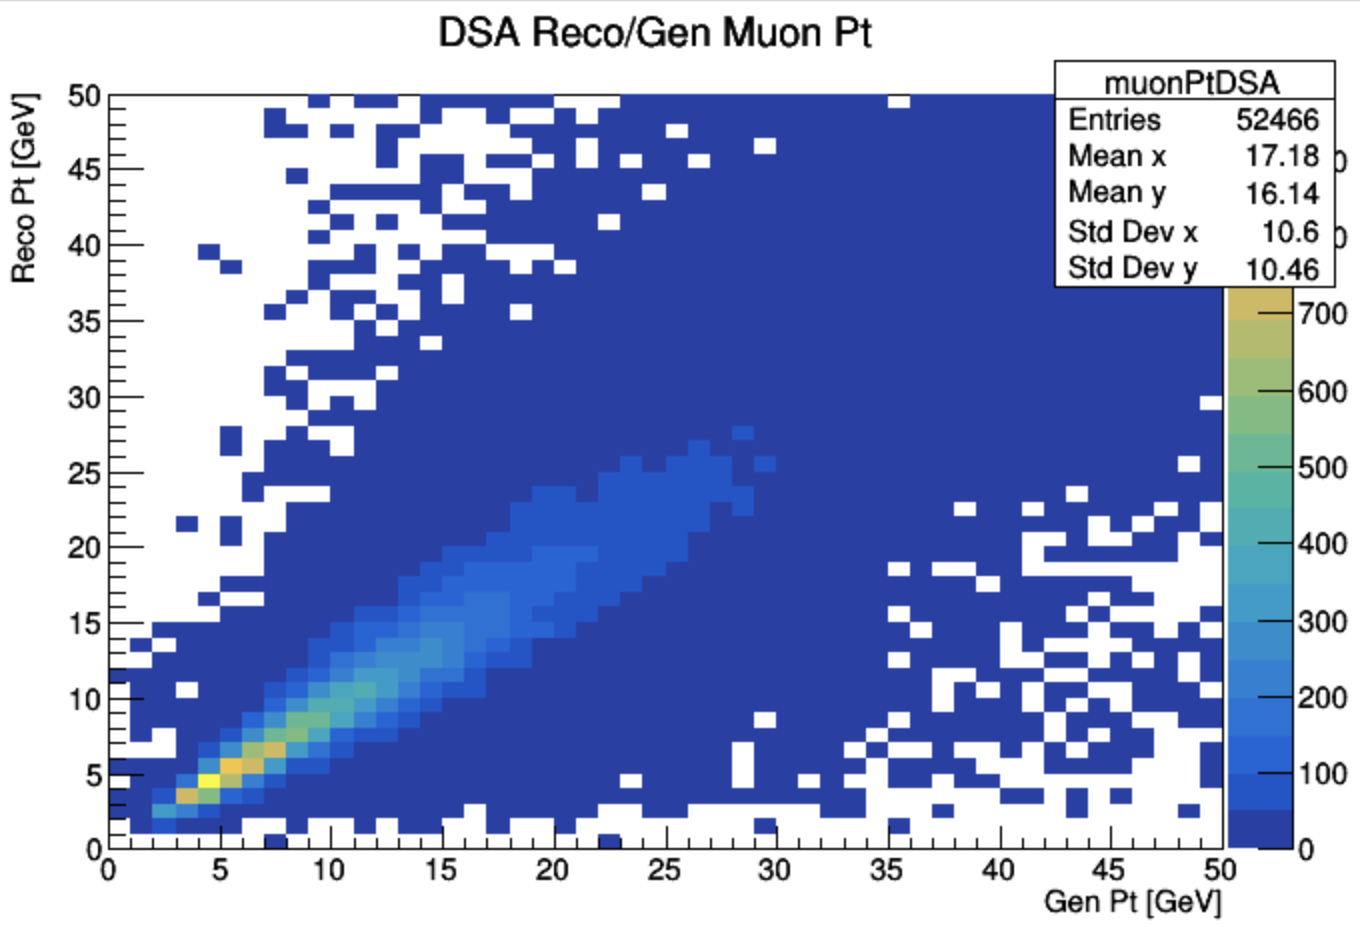
\includegraphics[width=12cm]{pT2D.png}
    \label{fig:12}
\end{figure}
\par
A comparative analysis of the gen muon pairs and the correspondingly reconstructed reco muon pairs can also be particularly instructive. With our requirement of initial state radiation, we expect the entire system to occupy a very compressed angular region. Therefore, we expect $\Delta$R($\mu_{\text{gen}}^{+}$, $\mu_{\text{gen}}^{-}$) to still be rather small, but remain an order of magnitude greater than $\Delta$R($\mu_{\text{gen}}^{+}$, $\mu_{\text{reco}}^{+}$) for example, which we have shown are largely kinematically identical. Figure~\ref{fig:13} provides the distributions of $\Delta$R($\mu_{\text{gen}}^{+}$, $\mu_{\text{gen}}^{-}$) and $\Delta$R($\mu_{\text{reco}}^{+}$, $\mu_{\text{reco}}^{-}$). These distributions largely verify our expectations. Not only are they both almost identical, but this $\Delta$R is an order of magnitude larger than that between the matched muons, though the still small overall. We made similar plots comparing the $\Delta$$\phi$ and $\Delta$$\eta$ between the reco pair and the gen pair, and again the distributions were almost identical.
\par
\begin{figure} [H]
\begin{subfigure}{.5\textwidth}
  \centering
  % include first image
  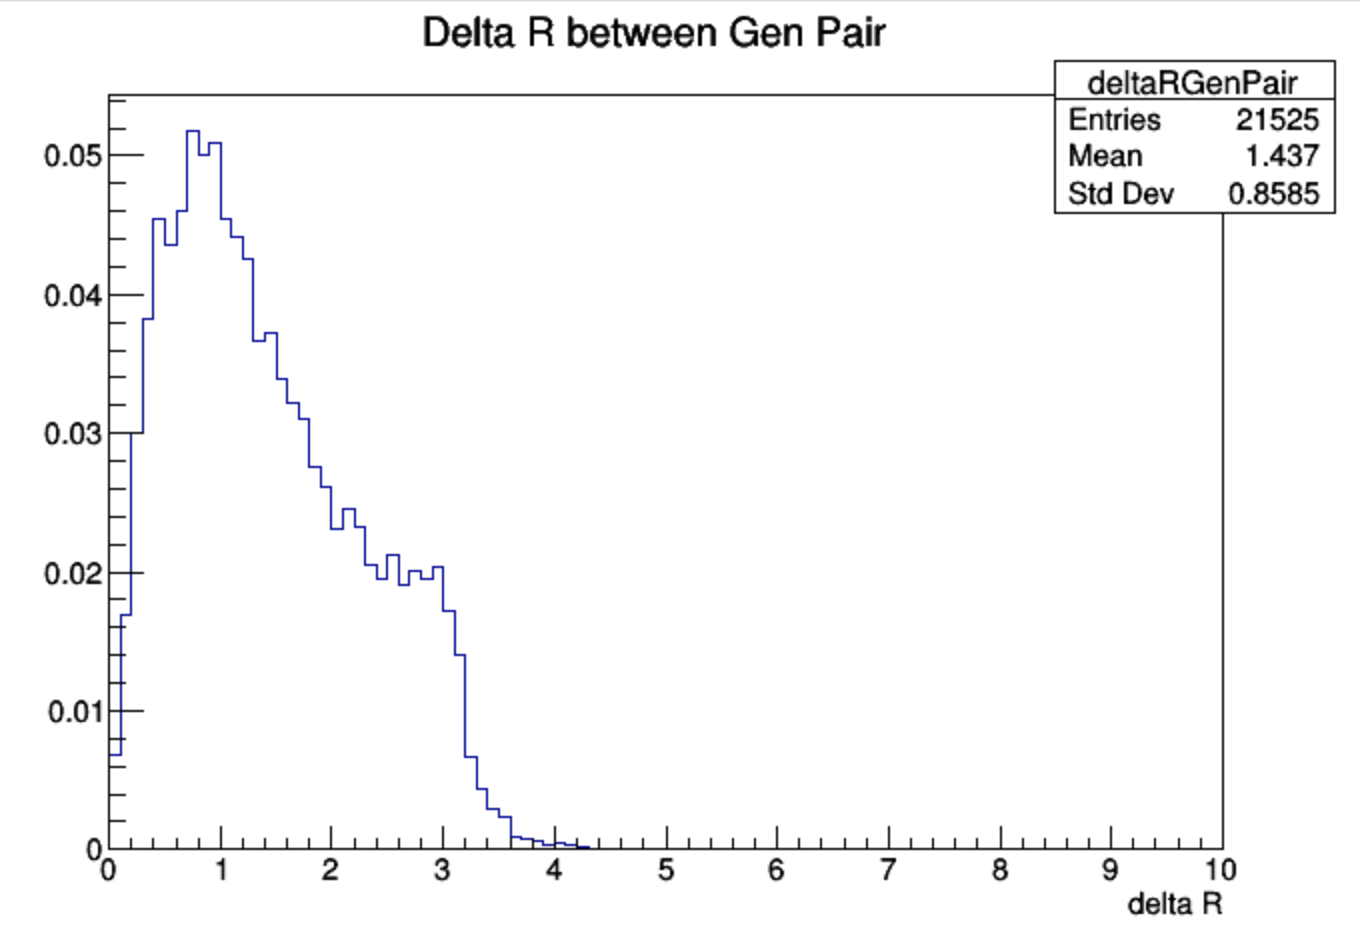
\includegraphics[width=.8\linewidth]{GenMuonsDeltaR.png}  
  \caption{$\Delta$R Distribution for Gen Pair}
  \label{fig:sub-first3}
\end{subfigure}
\begin{subfigure}{.5\textwidth}
  \centering
  % include second image
  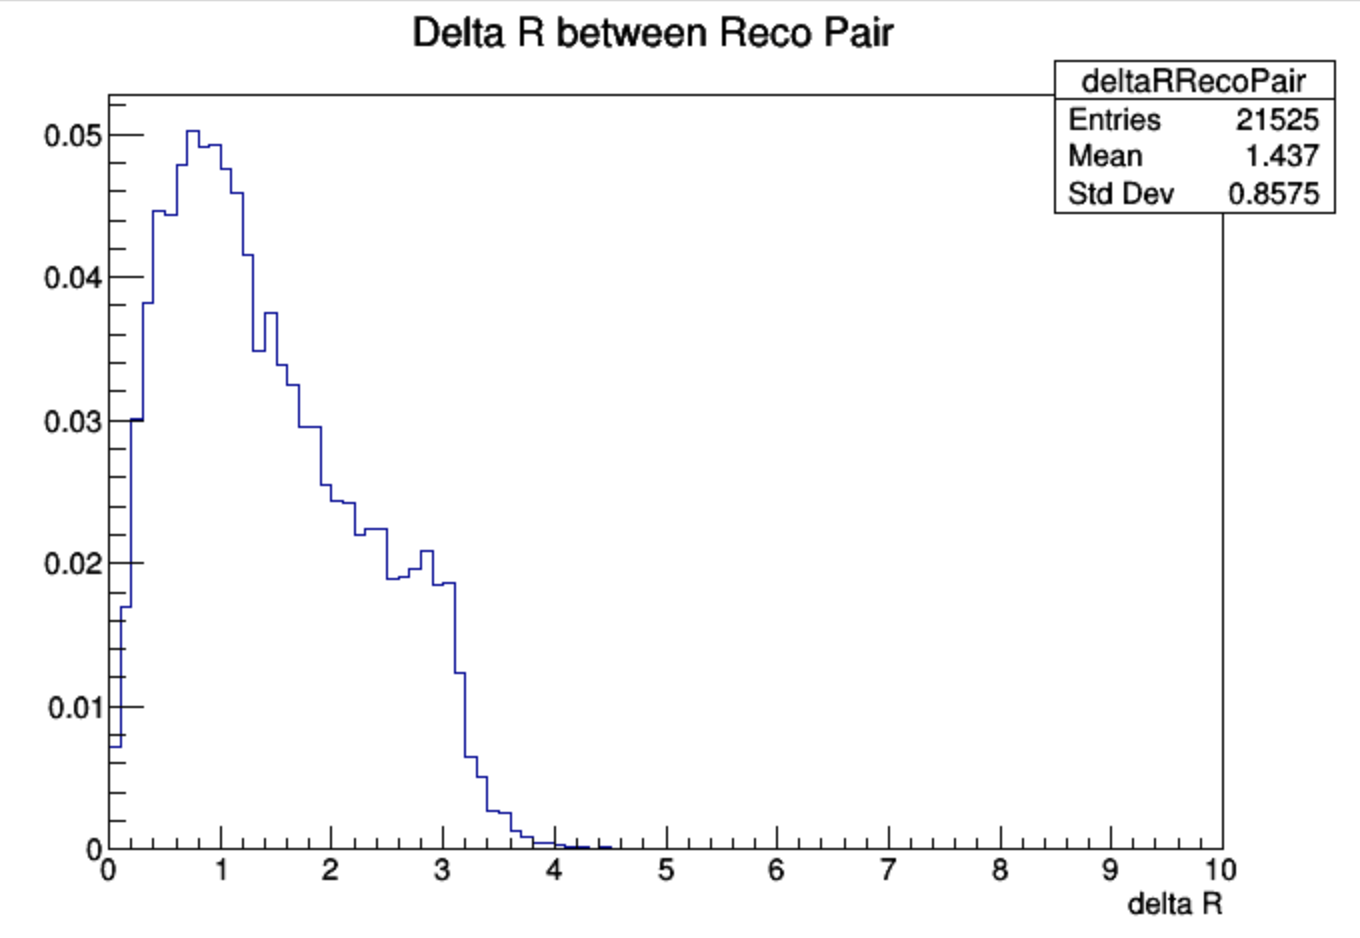
\includegraphics[width=.8\linewidth]{dSAMuonsDeltaR.png}  
  \caption{$\Delta$R Distribution for Reco Pair}
  \label{fig:sub-second3}
\end{subfigure}
\caption{}
\label{fig:13}
\end{figure}
\par
Recall that muon reconstruction is especially important as a means to reconstruct the Z$^{*}$, with the appropriate kinematic edge corresponding to the mass splitting between the $\chi_{2}^{0}$ and the $\chi_{1}^{0}$. Figure~\ref{fig:14} compares the reconstructed Z-mass when the gen muons are matched to either GM muons or dSA muons. The mass reconstruction accuracy is somewhat striking. The global muon pairs obey the expected kinematic edge, and almost identically matches the invariant mass given by the gen muons. However, the dSA muon distribution includes a considerable tail that passes surpasses the 30 GeV edge, highlighting the lack of track accuracy when inner tracker data is not included. This shows that at despite maintaining a very small angular separation between gen level and dSA matched muons, the variation in pT reconstruction, displayed in Figure~\ref{fig:12} can lead to inaccurate Z reconstruction. It is important to keep this feature in mind, as it largely inspires our later decision to focus on the "2 GM-dSA matched" data bin after applying reconstruction-level cuts. However, it should be noted that at larger ctaus, with which the expected displacement is on the same length scale as the inner tracker radius, the number of global muons will decrease by the corresponding order of magnitude, and matching gen muons to global muons is incredibly inefficient. In short, though matching gen and dSA muons is rather effective, the lack of pT resolution in dSA muons will later require us to only consider events in which both dSA tracks can be matched to a measured inner track. We'll show later that this eliminates a particularly large portion of the signal, but greatly improves discrimination against the background. With greater pT resolution in the muon chambers, or more efficient muon tracking in the inner tracker, a larger signal could have been discerned.
\begin{figure}[H]
    \centering
    \caption{Muon Pair Invariant Mass} 
    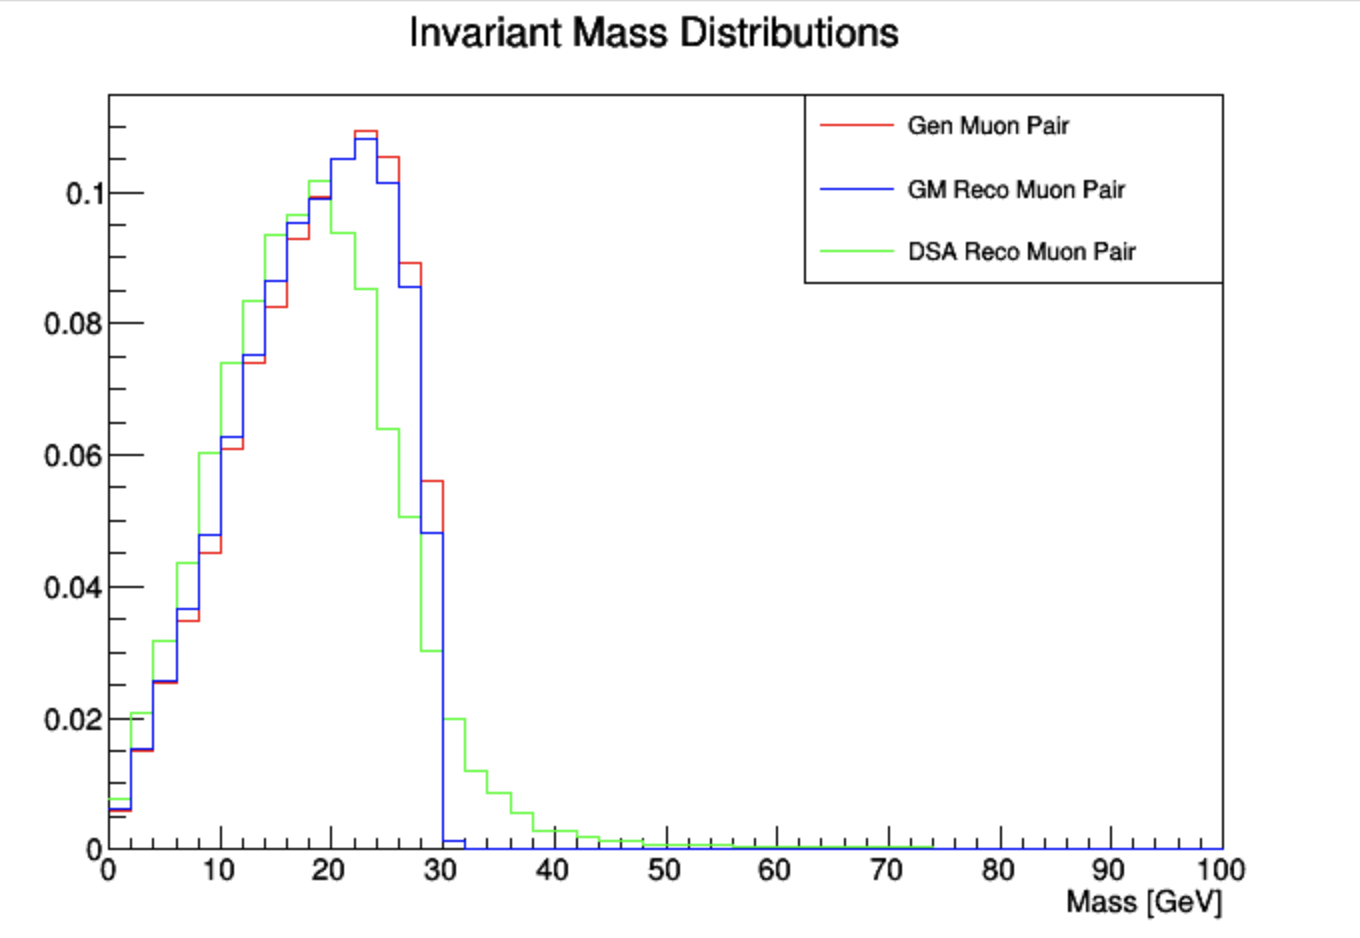
\includegraphics[width=12cm]{InvariantMassReco.png}
    \label{fig:14}
\end{figure}
\subsubsection{Other Reconstruction-Level Observations}
The MET is another essential metric regarding the reconstruction accuracy. By this stage, we've already applied a MET cut at gen level, eliminating all events for which MET $<$ 80 GeV. It is important to verify that this largely corresponds with reco-level MET $<$ 80 GeV as well. In short, if our gen-level cuts do not translate well to our reconstruction-level observables, then it is difficult to assert that what we measure in the detector can be used to prove or disprove the idealized process we've simulated at gen-level. Moreover, in this particular process, the reconstructed MET serves as a proxy measurement for the LSPs - inadequate MET reconstruction drastically reduces our sensitivity to this SUSY signal. Figure~\ref{fig:15} provides several figures that delineate the effectiveness of MET reconstruction. Similar to the muon matching pT plot, in an idealized reconstruction scenario, all points lie near the line for which the reco MET equals the gen MET. The presence of the gen-level MET cut is apparent by the edge at 80 GeV - however, there are many events for which the reco MET is substantially less than 80 GeV. The 1D histograms in the figure show are the projections of the 2D histogram in along either the x or y axis. The prominent tail below 80 GeV for the reco MET signifies the extent to which misreconstruction affects our analysis.
\par
\begin{figure}
\begin{subfigure}[b]{.3\textwidth}
  \centering
  % include first image
  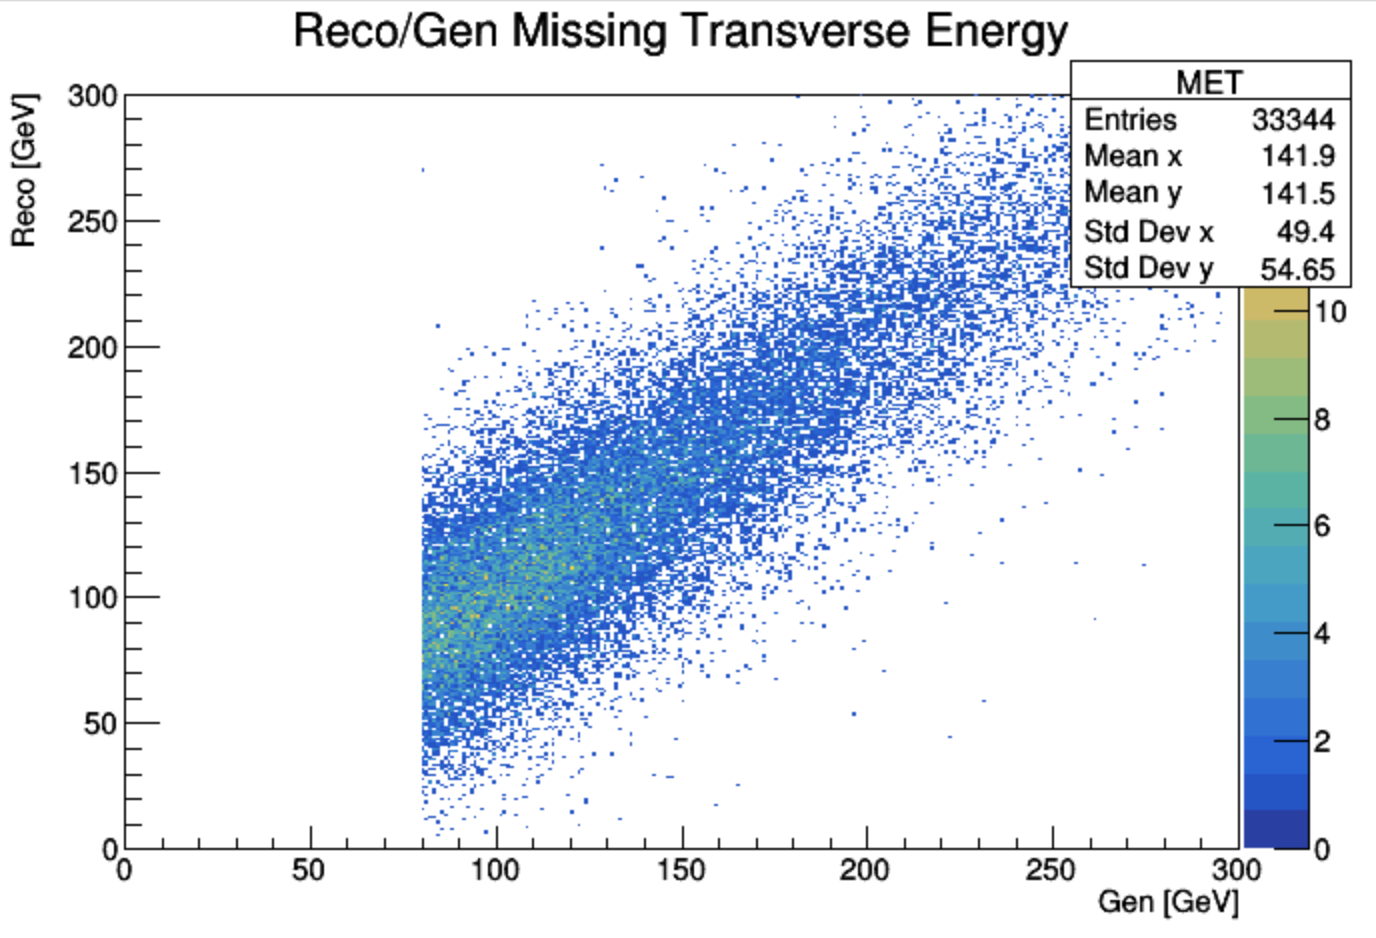
\includegraphics[width=\textwidth]{MET2D.png}  
  \caption{Gen/Reco MET}
  \label{fig:sub-first2D}
\end{subfigure}
\begin{subfigure}[b]{.3\textwidth}
  \centering
  % include third image
  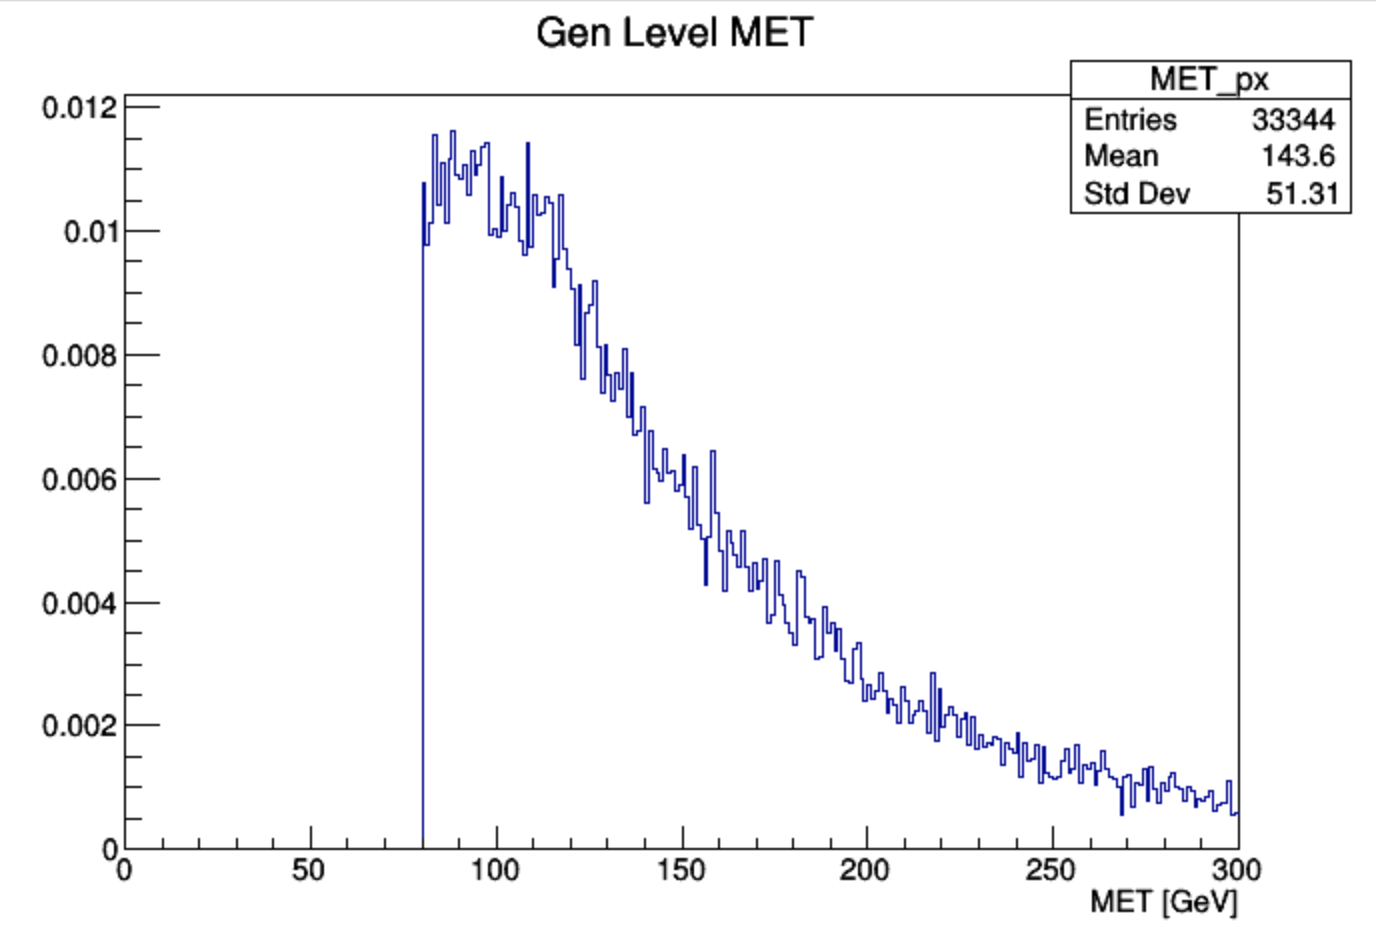
\includegraphics[width=\textwidth]{METGen.png}  
  \caption{Gen MET}
  \label{fig:sub-thirdgen}
\end{subfigure}
\begin{subfigure}[b]{.3\textwidth}
  \centering
  % include fourth image
  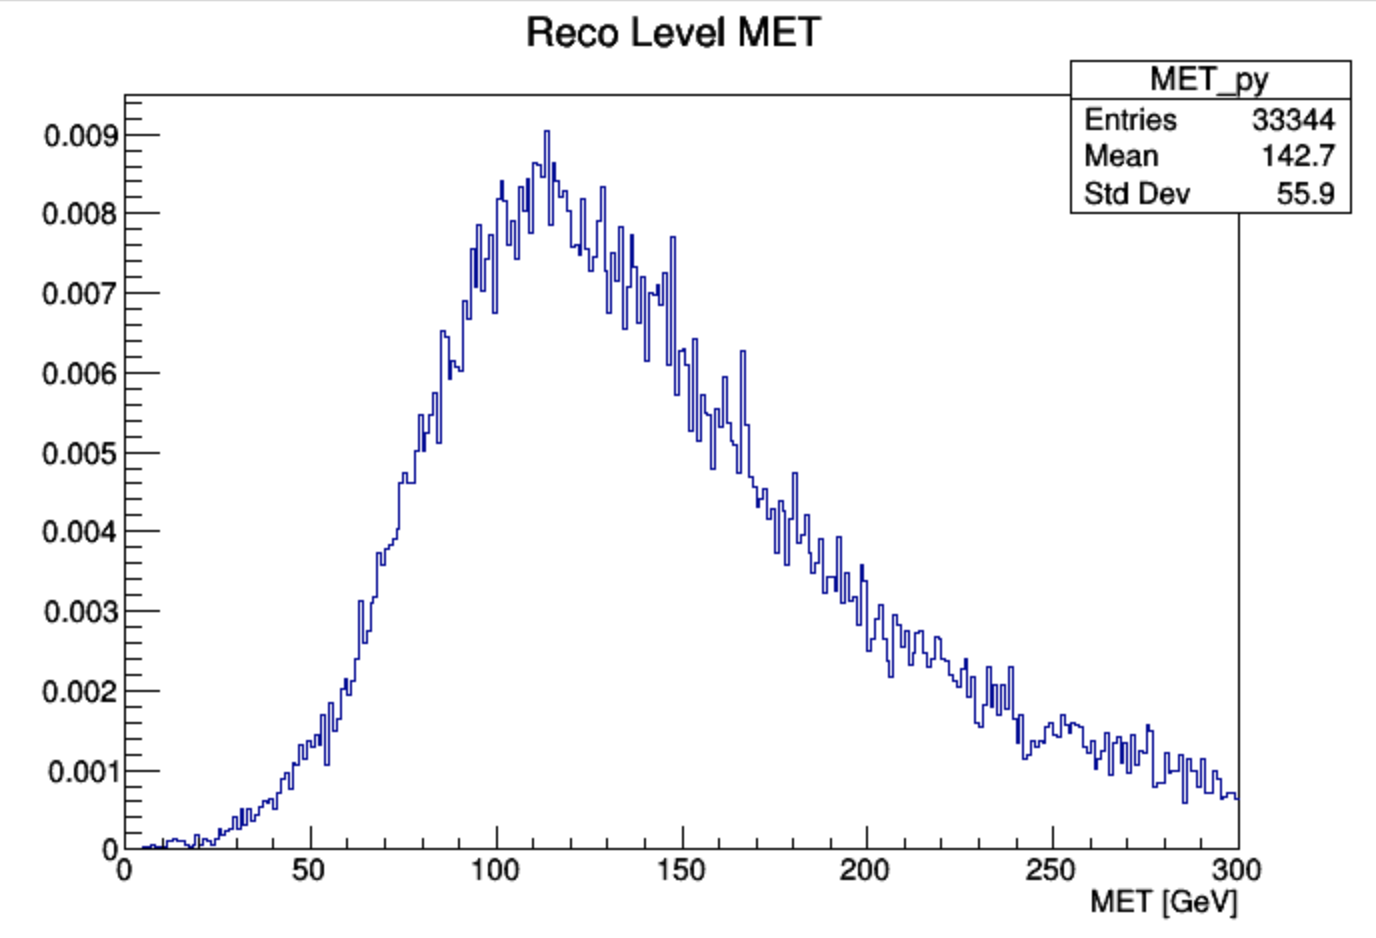
\includegraphics[width=\textwidth]{METReco.png}  
  \caption{Reco MET}
  \label{fig:sub-fourthgen}
\end{subfigure}
\caption{MET Reconstruction Distributions}
\label{fig:15}
\end{figure}
As specified earlier, MET is usually computed by adding the vector sum of the detected particles from a given event. We've found that pT reconstruction for muons is not necessarily optimized, it is reasonable to expect that the pT sum is somewhat inaccurate, leading to a non-ideal reconstructed MET. However, overall we have found that reconstruction has generally been quite effective, and we were willing to apply reconstruction-level cuts and continue our analysis.
\subsection{Dimuon Mass Reconstruction and Signal Region Identification}
The analysis code supplied by the IDM group outputted a variety of histograms, such as the kinematics of the ISR jet and the reconstructed muons. However, we focused on the Dimuon mass distribution, whose kinematic edge could most directly signifies the presence of two Neutralinos with a well-defined mass splitting. We'll show that this particular observable allowed us to find a well-defined signal region with minimal background. It should be noted that most searches, including CMS's IDM search, the researchers focus only on the number of events that pass a given set of cuts, without considering the shape of the distribution that results from measuring the attributes of the remaining events. However, we don't ``blind" our analysis as they do. We also consider the shape of our distribution as a means to inform additional cuts and regions of interest - we hope that this way we can inform these groups of potentially helpful modifications to their analysis without compromising the integrity of their method.
\par
Figure~\ref{fig:16} displays the dimuon mass distribution without the application of cuts for the Wino/Bino scenario with a $\chi_{2}^{0}$ mass of 125 GeV and the $\chi_{1}^{0}$ mass of 115 GeV. We made the same set of plots for all mass configurations of both the Higgsino and Wino/Bino scenarios. All background is simulated, and we use the 2018 Run 2 luminosity of 59.74 fb$^{-1}$ when computing the number of events. We use this luminosity for all plots in this sections, and it should be noted that the total number of both signal and background events would be more than doubled if we considered the entirety of Run 2 data. 
\begin{figure}[H]
    \centering
    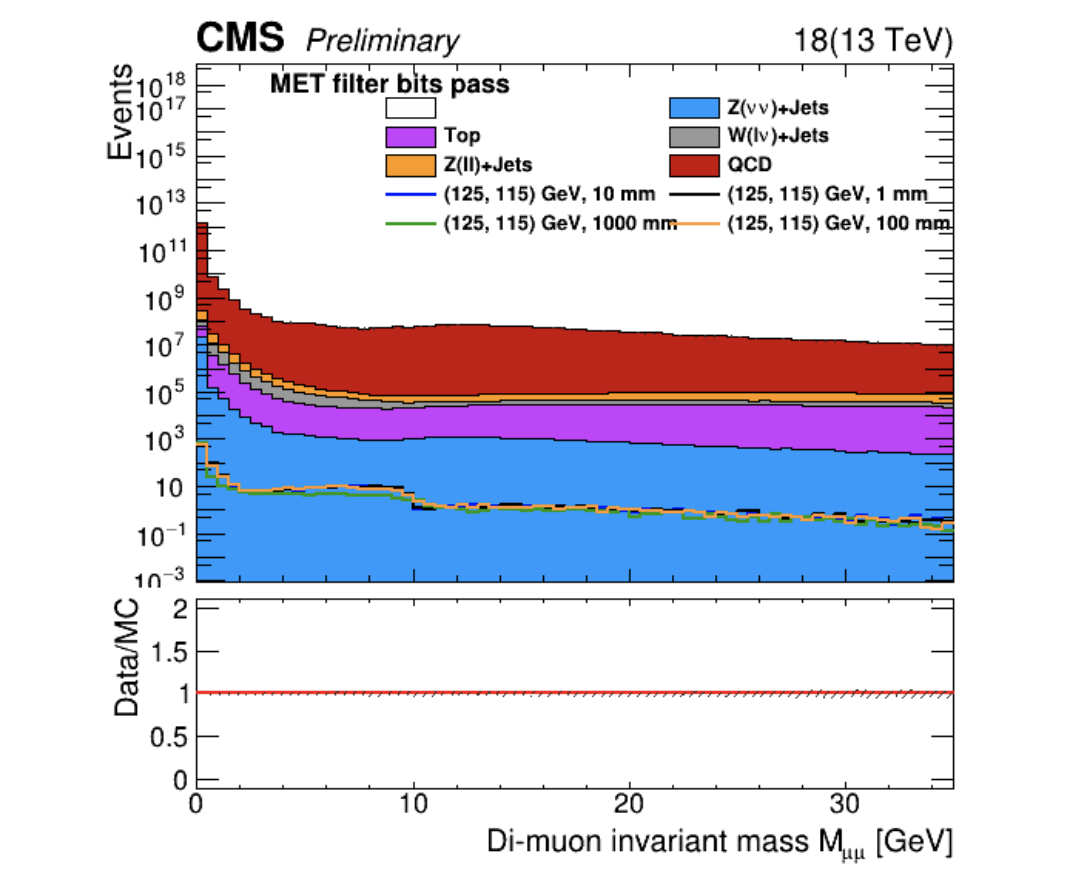
\includegraphics[width=12cm]{NoCuts.png}
    \caption{Example Dimuon Mass Distribution with no Reco-Level Cuts} 
    \label{fig:16}
\end{figure}
\par
Clearly, it is largely hopeless to discern any signal without finding a means to eliminate background. Moreover, from the stacked background and logscale y-axis, mis-reconstructed QCD is clearly the predominant source of background. However, the distribution dramatically changes after applying the cuts listed in the reco-level cuts section. Table~\ref{table:4} shows the number of events that pass each cut for all 4 ctaus for this particular signal (note that these efficiencies are largely the same for each signal sample). 
    \begin{table}[H]
        \centering
        \begin{tabular}{||c|c|c|c|c|c||}
            \hline
            Cut# & Description & 1000 mm & 100 mm & 10 mm & 1 mm \\
            \hline
            cut0 & No cuts & 843.525 & 853.746 & 844.113 & 845.923 \\
            cut1 & MET filter bits pass & 843.28 & 853.526 & 843.917 & 845.587 \\
            cut2 & HEM veto & 815.019 & 824.877 & 814.975 & 816.127 \\
            cut3 & Trigger fired (120 GeV METNoMu) & 395.084 & 402.918 & 399.523 & 399.259 \\
            cut4 & MET $>$ 200 GeV & 224.365 & 216.763 & 208.252 & 207.342 \\
            cut5 & $|$CaloMET - PFMET$/$CaloMET $<$ 1 & 223.459 & 216.133 & 207.646 & 206.802 \\
            cut6 & nJets $>$ 0 (pT $>$ 30 GeV) & 220.607 & 213.165 & 204.808 & 203.928 \\
            cut7 & leading jet $|$#eta$|$ $<$ 2.4 & 214.084 & 207.222 & 199.274 & 199.053 \\
            cut8 & Leading jet pT $>$ 80 GeV & 210.531 & 203.272 & 195.604 & 195.804 \\
            cut9 & $|$#Delta#Phi(MET, leading jet)$|$ $>$ 1.5 & 209.438 & 202.003 & 194.409 & 194.87 \\
            cut10 & $|$#Delta#Phi(MET, all jets)$|$ $>$ 0.5 & 184.06 & 175.413 & 168.89 & 167.406 \\
            cut11 & nJets $<$ 3 (pT $>$ 30 GeV) & 125.84 & 119.312 & 113.153 & 111.291 \\
            cut12 & 0 b-tagged jets (w SF) & 125.84 & 119.312 & 113.153 & 111.291 \\
            cut13 & good dSA muons $>=$ 1 & 83.4213 & 88.9282 & 84.3507 & 84.4195 \\
            cut14 & good dSA muons $>=$ 2 & 30.1089 & 32.6092 & 31.9094 & 31.3928 \\
            cut15 & best\_dsa\_0 $!=$ best\_dsa\_1 & 17.7391 & 30.8976 & 30.1997 & 29.8633 \\
            cut16 & Cosmic veto (min(cosalpha) $>$ -0.94) & 16.1682 & 28.3201 & 27.6459 & 27.5956 \\
            cut17 & good dSA-dSA vertex $>=$ 1 & 16.1682 & 28.3201 & 27.6459 & 27.5956 \\
            cut18 & Best dSA 0 pT resolution $<$ 1 & 16.1682 & 28.3201 & 27.6459 & 27.5956 \\
            cut19 & Best dSA 1 pT resolution $<$ 1 & 16.1682 & 28.3201 & 27.6459 & 27.5956 \\
            cut20 & Vertex #chi$^{2}$ $<$ 4 & 9.38282 & 18.7211 & 19.2301 & 19.5052 \\
            cut21 & MT $<$ 200 GeV & 9.35661 & 18.6677 & 19.2035 & 19.3989 \\
            cut22 & M_{$\mu\mu$} $<$ 30 GeV & 8.98476 & 18.2411 & 18.9939 & 18.8791 \\
            cut23 & dR(muons) $<$ 0.9 & 5.66734 & 13.2661 & 13.9578 & 14.2526 \\
            cut24 & muons: OSSF & 5.50508 & 12.8327 & 13.7943 & 13.9292 \\
            cut25 & Selected muon 0 dxy $>$ 0.1 cm & 5.39582 & 11.8212 & 9.31867 & 1.61764 \\
            cut26 & Selected muon 1 dxy $>$ 0.1 cm & 5.34241 & 11.3451 & 7.74777 & 0.745311 \\
            cut27 & 0 GM-dSA matched & 2.96067 & 1.78446 & 0.0862716 & 0.027152 \\
            cut28 & 1 GM-dSA matched & 0.915207 & 3.37212 & 0.968559 & 0.13215 \\
            cut29 & 2 GM-dSA matched & 1.46654 & 6.1885 & 6.69294 & 0.586009 \\
            \hline
        \end{tabular}
        \caption{Cutflow Efficiency for 125 GeV $\chi_{2}^{0}$ and 115 GeV $\chi_{1}^{0}$} sample
        \label{table:4}
    \end{table}
From the table, it is clear that the majority of events are lost due to insufficient MET and a lack of good dSA muons. Furthermore, after applying cuts, we lose more events with an especially small lifetime (ctau = 1 mm) due to their small transverse displacement (dxy) within the detector. We computed similar cutflow tables for all types of background, which we won't include here for the sake of brevity.
\par
Next, we investigated the signal and background distribution in each of our GM-dSA matching bins denoted cut27, cut28, and cut29 in the above table. Again these are $\textbf{not}$ inclusive cuts. Figure~\ref{fig:17} shows the distributions in each bin for the 25 GeV $\chi_{2}^{0}$ and 115 GeV $\chi_{1}^{0}$ sample.
par
\begin{figure}
\begin{subfigure}[b]{.3\textwidth}
  \centering
  % include first image
  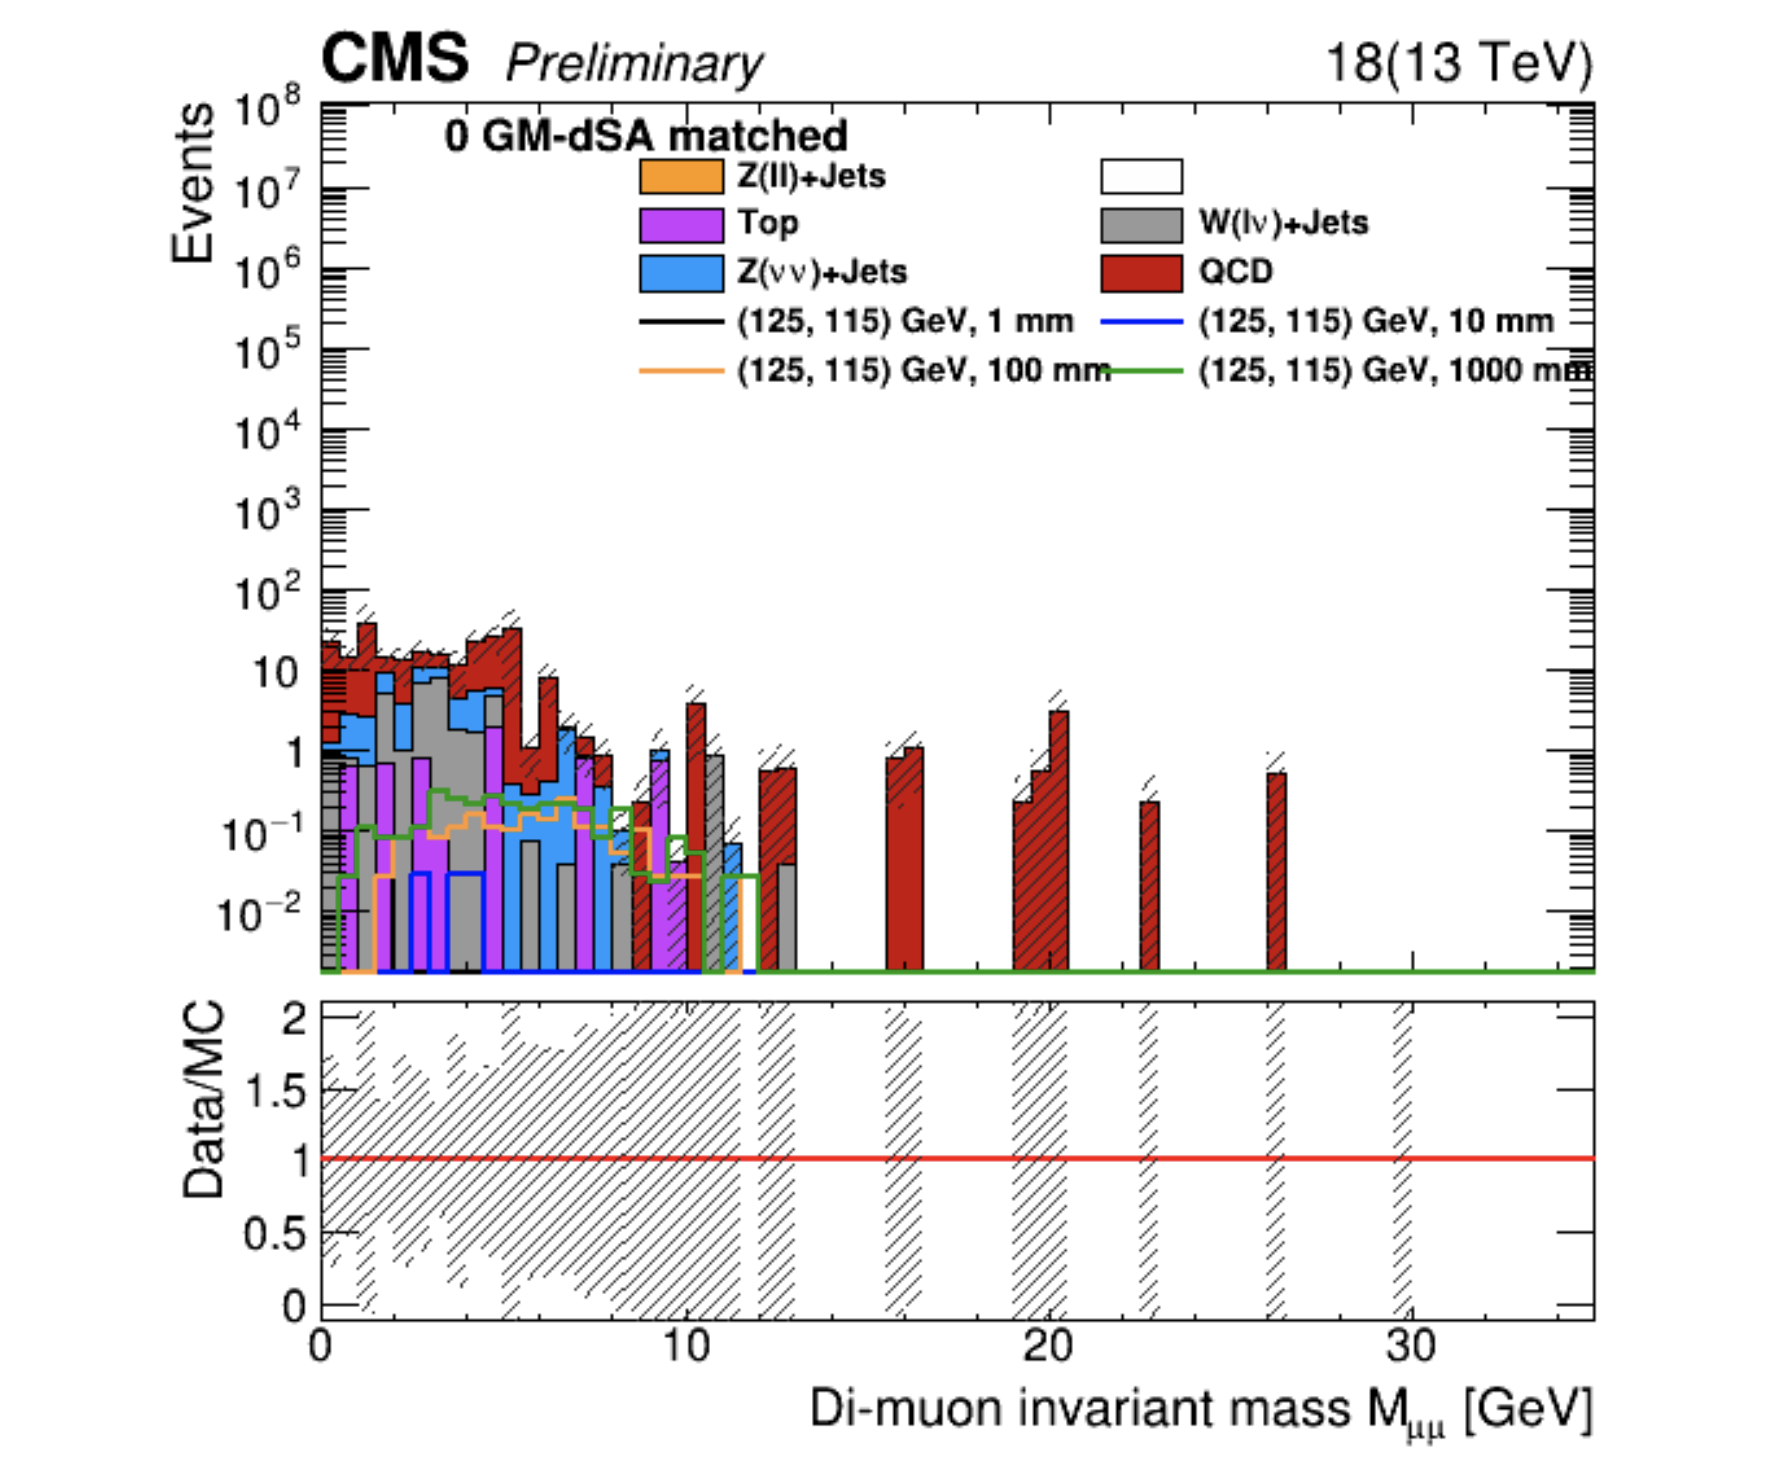
\includegraphics[width=\textwidth]{Cut27.png}  
  \caption{0 GM-dSA matched}
  \label{fig:sub-first27}
\end{subfigure}
\begin{subfigure}[b]{.3\textwidth}
  \centering
  % include third image
  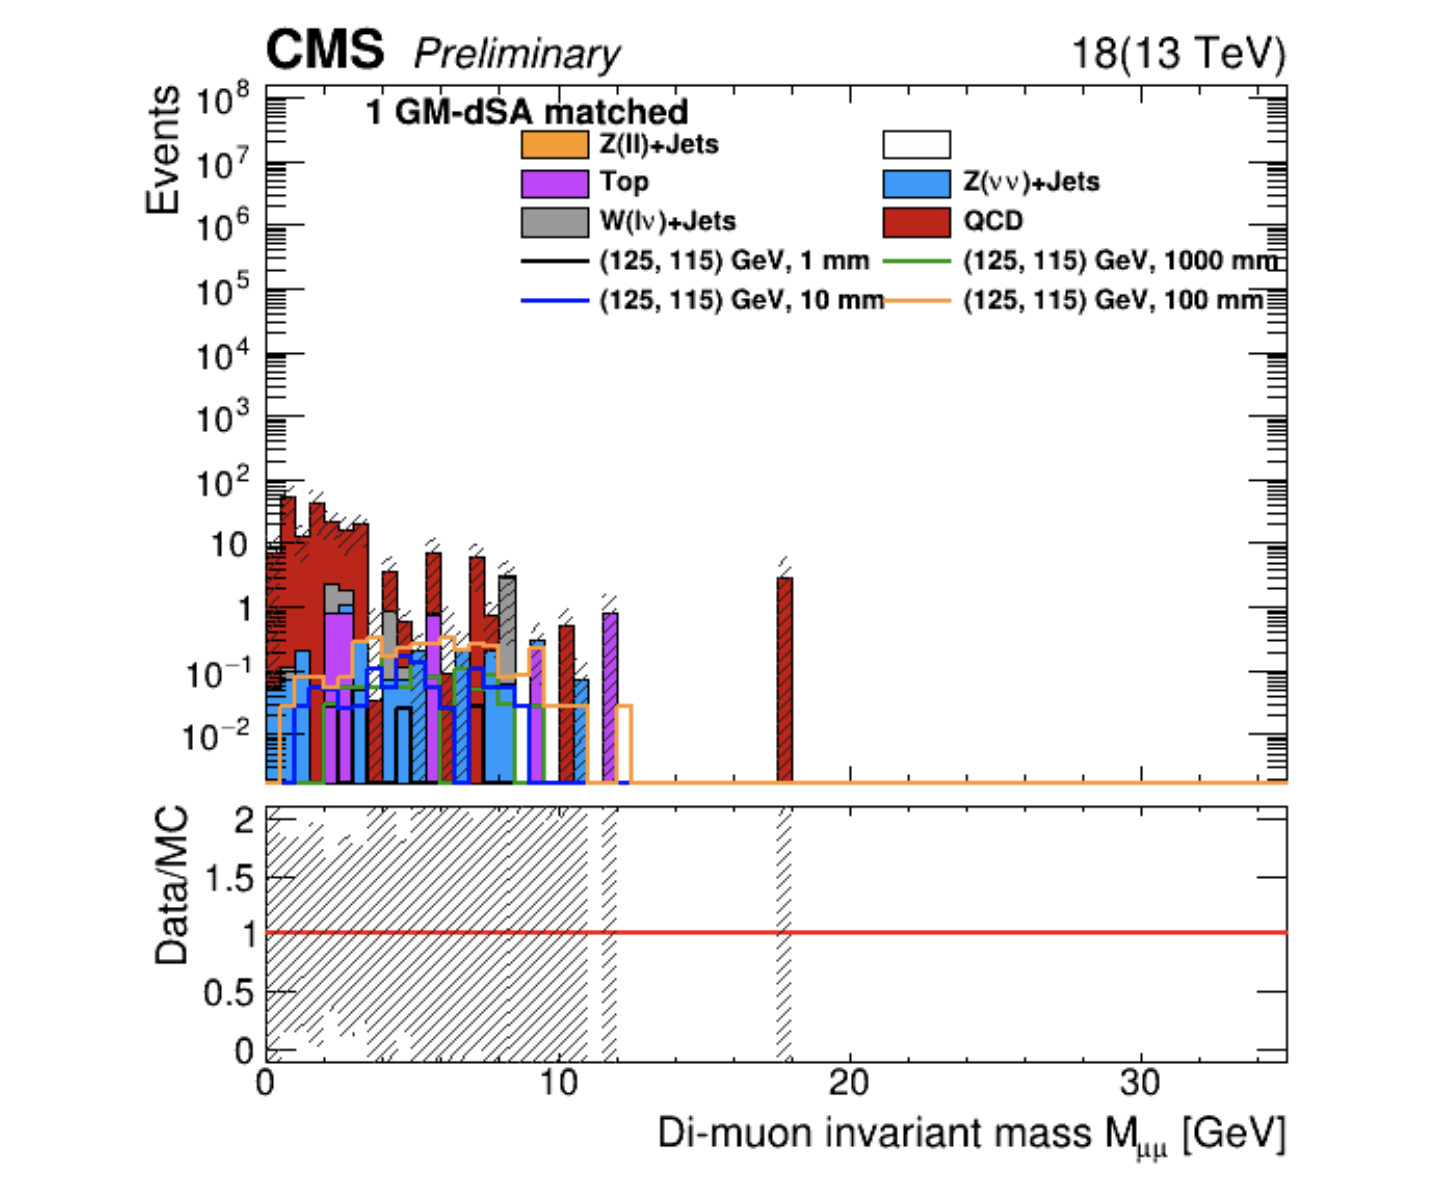
\includegraphics[width=\textwidth]{Cut28.png}  
  \caption{1 GM-dSA matched}
  \label{fig:sub-third28}
\end{subfigure}
\begin{subfigure}[b]{.3\textwidth}
  \centering
  % include fourth image
  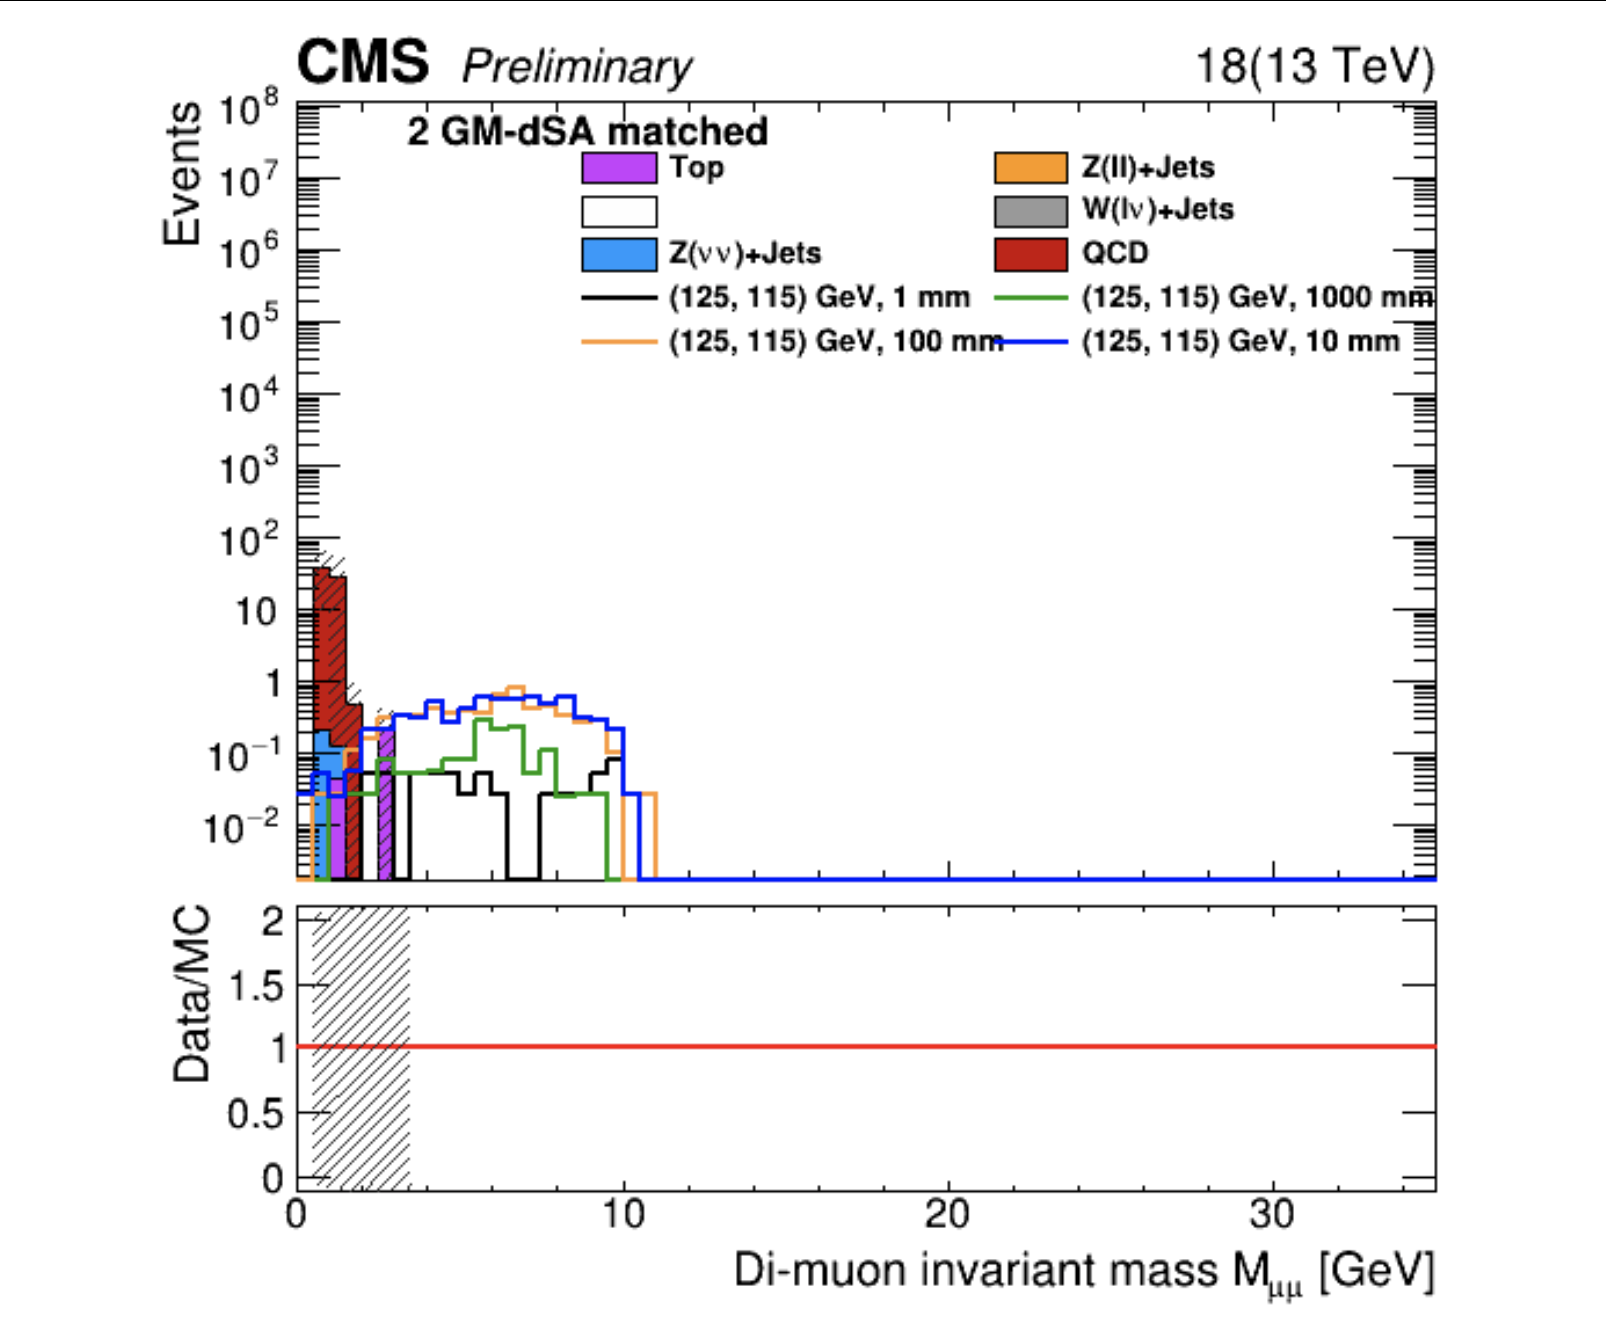
\includegraphics[width=\textwidth]{Cut29.png}  
  \caption{2 GM-dSA matched}
  \label{fig:sub-fourth29}
\end{subfigure}
\caption{Muon Track Matching Bins}
\label{fig:17}
\end{figure}
\par
From Figure~\ref{fig:17}, it should be clear that we can only establish a clean signal region with no background in the 2 GM-dSA matched bin. This is somewhat expected - by requiring that both muons have tracks in the inner tracker, we greatly reduce the presence of misreconstructed background at higher dimuon mass values - we can effectively ``trust" the given events in this bin do indeed involve two real muons with the desired kinematics. As a result, we effectively included an additional last cut in which we would only analyze events with 2 GM-dSA matched muons.
\par
Briefly, we'll quantitatively examine how the shape of the signal region changes with the mass splitting. Figure~\ref{fig:18} shows the dimuon mass distribution after applying all reco-level cuts, including 2 GM-dSA matched, for N2C1 Higgsino samples with a 100 GeV $\chi_{1}^{0}$ mass. 
\par
\begin{figure} [H]
\begin{subfigure}{.5\textwidth}
  \centering
  % include first image
  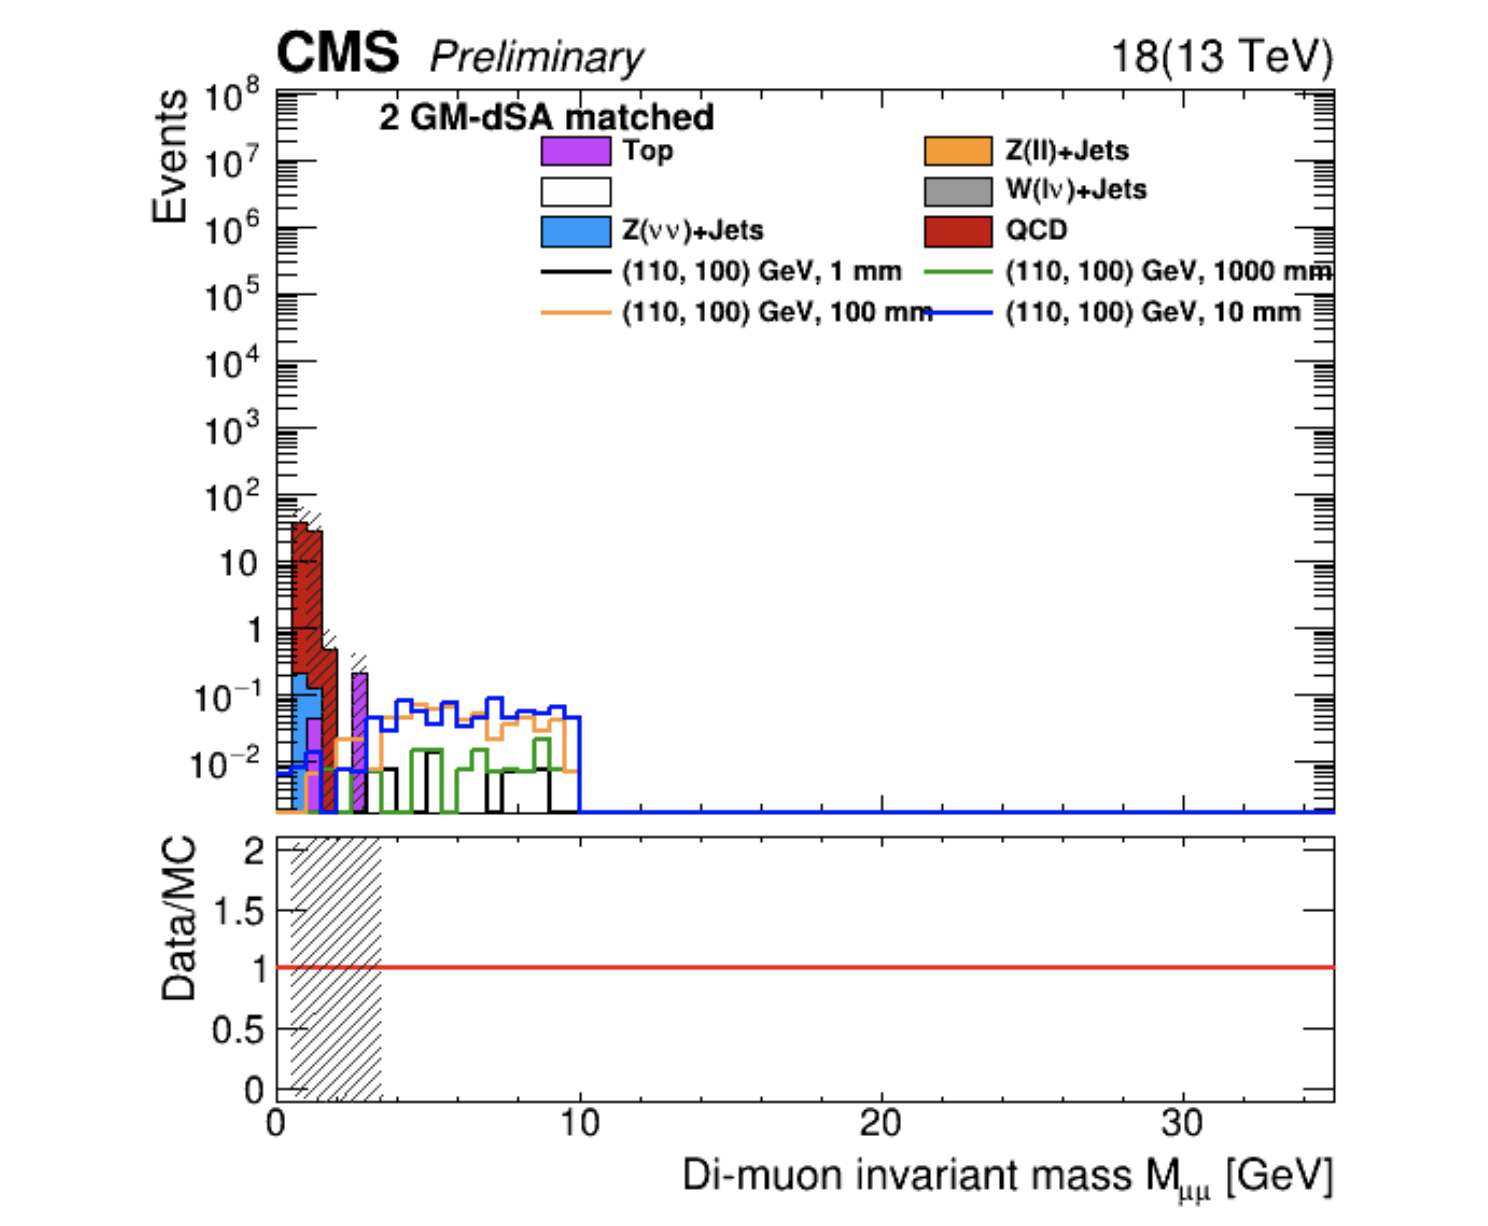
\includegraphics[width=.8\linewidth]{Split10.png}  
  \caption{10 GeV Neutralino Mass Splitting}
  \label{fig:sub-first18}
\end{subfigure}
\begin{subfigure}{.5\textwidth}
  \centering
  % include second image
  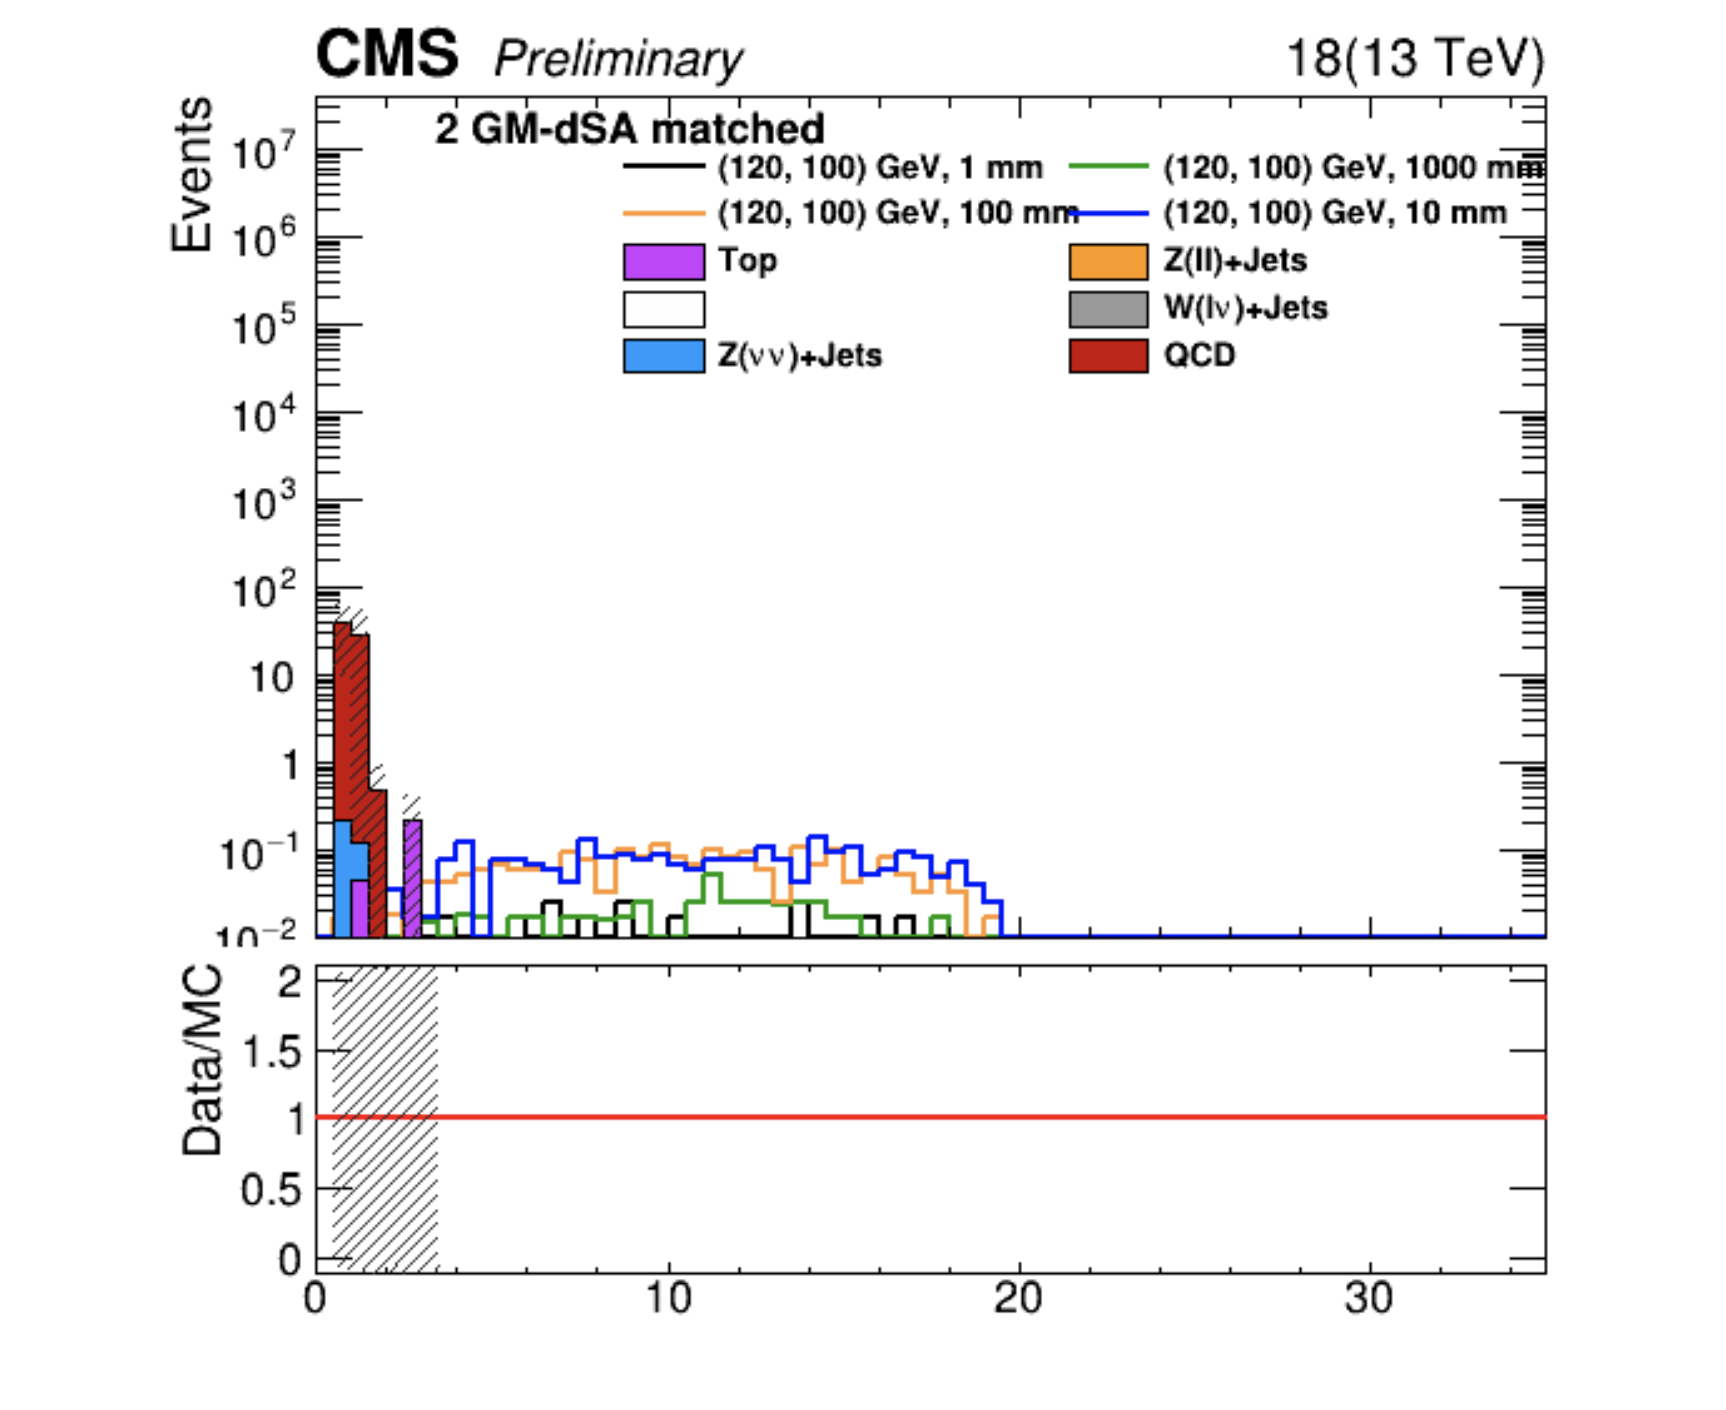
\includegraphics[width=.8\linewidth]{Split20.png}  
  \caption{20 GeV Neutralino Mass Splitting}
  \label{fig:sub-second18}
\end{subfigure}
\begin{subfigure}{.5\textwidth}
  \centering
  % include third image
  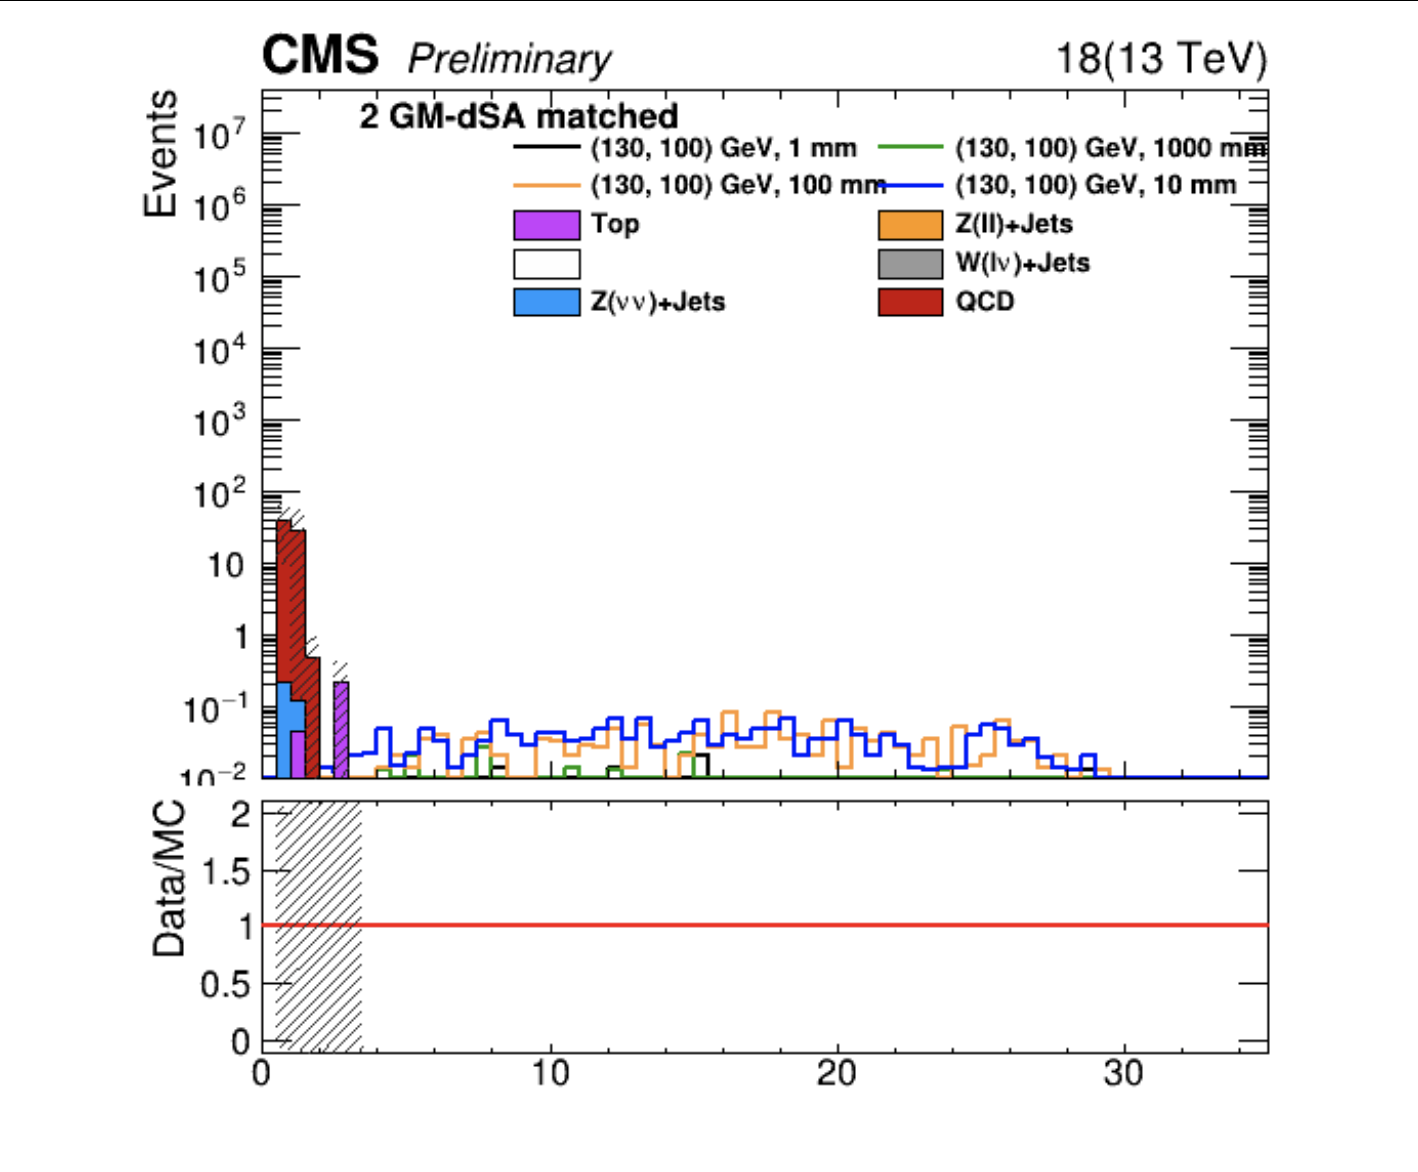
\includegraphics[width=.8\linewidth]{Split30.png}  
  \caption{30 GeV Neutralino Mass Splitting}
  \label{fig:sub-third18}
\end{subfigure}
\begin{subfigure}{.5\textwidth}
  \centering
  % include fourth image
  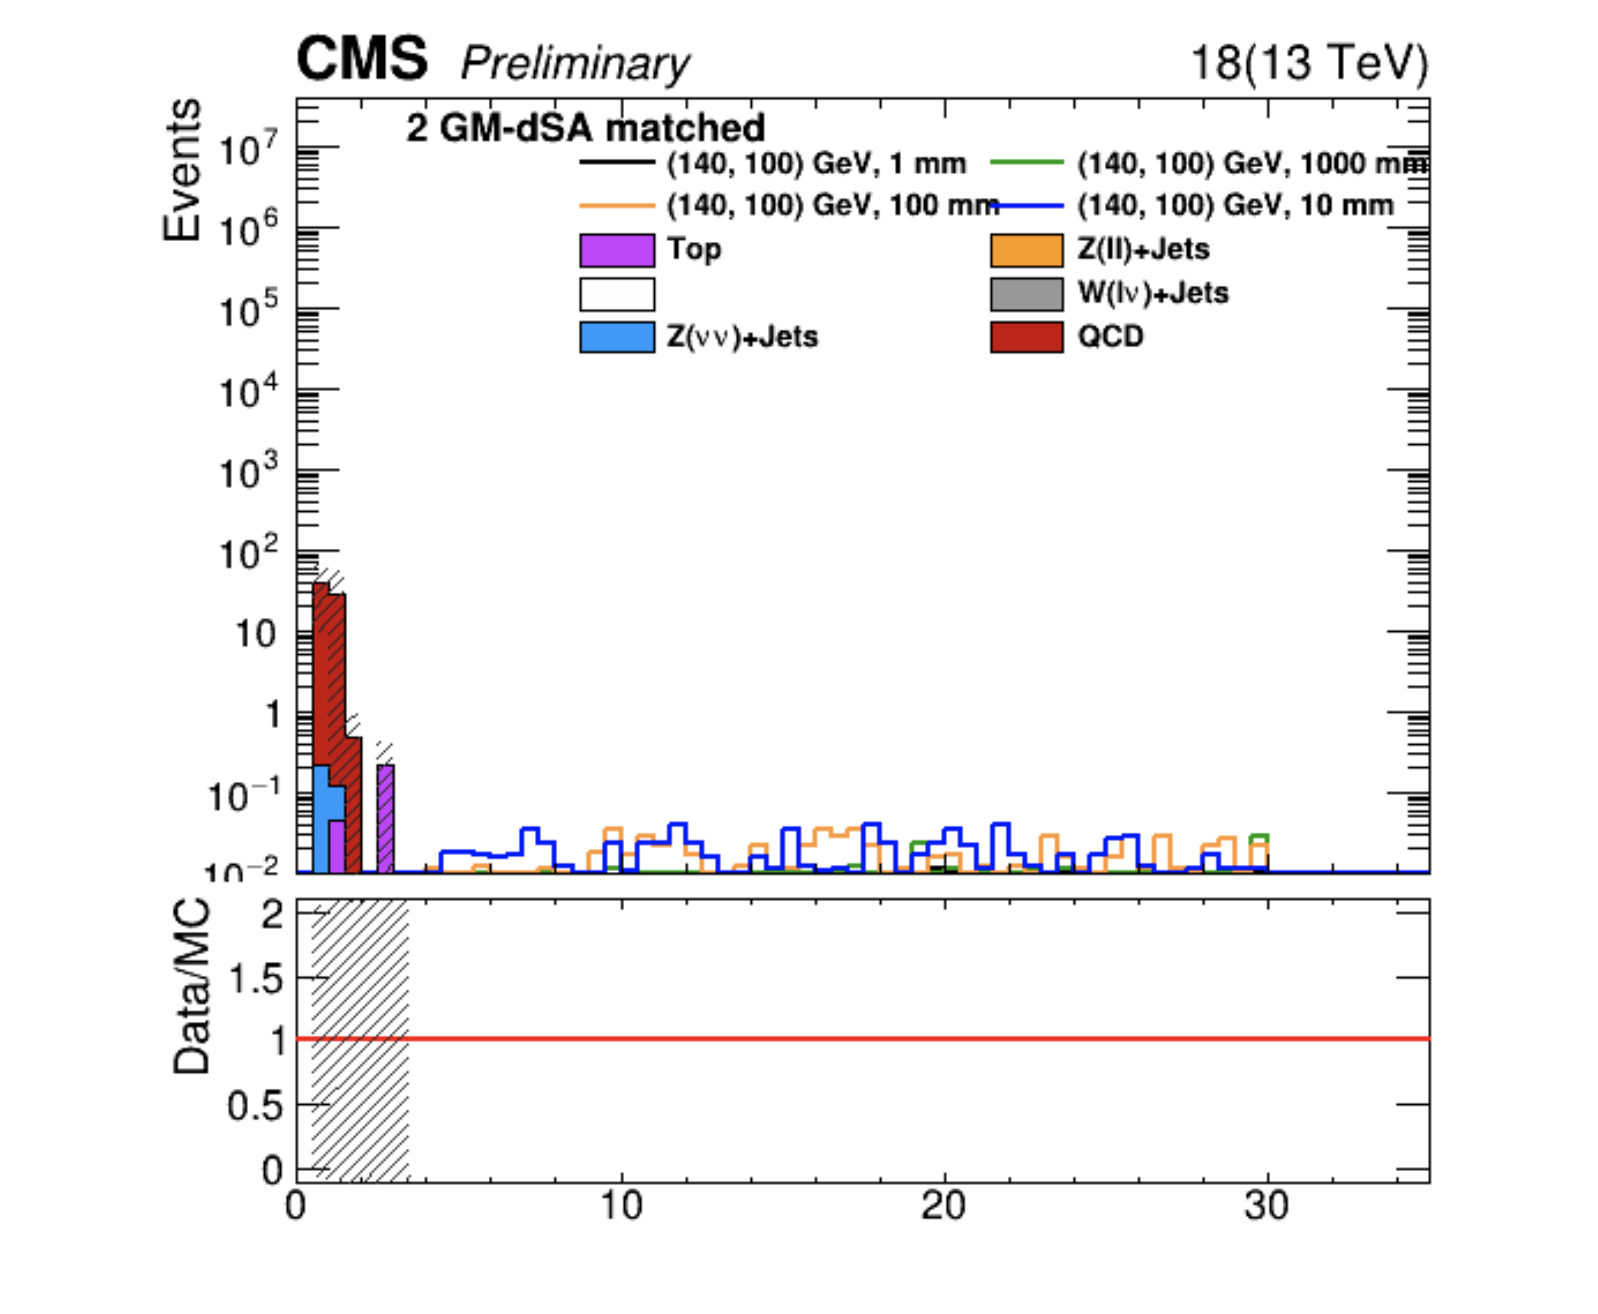
\includegraphics[width=.8\linewidth]{Split40.png}  
  \caption{40 GeV Neutralino Mass Splitting}
  \label{fig:sub-fourth18}
\end{subfigure}
\caption{Signal/Background Plots for 100 GeV $\chi_{1}^{0}$ N2C1 Higgsino Samples}
\label{fig:18}
\end{figure}
\par
As expected, the distribution includes a kinematic edge that corresponds with the neutralino mass splitting aside from the 40 GeV case, as a reco-level cut is applied on a dimuon mass values greater than 30 GeV. The larger the mass splitting, the more flat the histogram, as a similar number of events is distributed over a wider spread in mass. The 40 GeV has less events in the signal region than the 30 GeV case, as a portion are substantial portion of events are removed with the 30 GeV cut. Otherwise, the total number of plotted events seems of the same order of magnitude for the different mass splittings, with the predominant differences being between different ctau values.
\par
Thus, we define our signal region for a given sample as the the set of events between 3 GeV and the kinematic edge. This removes all background while maximizing the number of signal events. We therefore can integrate our histograms within this region to find the number of expected events for a given mass configuration and ctau. In the Higgsino case, we add the events in the N2C1 and N2N1 distributions, and propagate the uncertainty accordingly. 
\begin{table}[H]
        \centering
        \begin{tabular}{||c|c|c|c|c||}
        \hline
        {$\chi_{2}^{0}$ mass}\_{$\chi_{1}^{0}$ mass} & 1 mm Events & 10 mm Events & 100 mm Events & 1000 mm Events \\
        \hline
        110\_100	& 0.289 +- 0.052 & 2.722 +- 0.163 & 2.918 +- 0.167 & 0.547 +- 0.073 \\
        120\_100	& 0.352 +- 0.053 & 2.856 +- 0.149 & 3.205 +- 0.158 & 0.623 +- 0.070 \\
        130\_100	& 0.254 +- 0.040 & 2.055 +- 0.114 & 2.438 +- 0.125 & 0.405 +- 0.050 \\
        140\_100	& 0.132 +- 0.027 & 1.046 +- 0.075 & 1.168 +- 0.079 & 0.302 +- 0.103 \\
        \hline
        \hline
        135\_125 & 0.109 +- 0.022 & 1.268 +- 0.080 & 1.432 +- 0.085 & 0.282 +- 0.038 \\
        145\_125	& 0.176 +- 0.028 & 1.800 +- 0.088	& 1.899 +- 0.091 & 0.434 +- 0.044 \\
        155\_125	& 0.101 +- 0.019 & 1.211 +- 0.066 & 1.303 +- 0.298 & 0.293 +- 0.032 \\
        165\_125	& 0.127 +- 0.019 & 0.726 +- 0.047 & 0.782 +- 0.049 & 0.191 +- 0.025 \\
        \hline
        \end{tabular}
        \caption{Signal Region Events in Higgsino Scenario}
        \label{table:5}
\end{table}
\par
Similarly, for the Wino/Bino Case:
\begin{table}[H]
        \centering
        \begin{tabular}{||c|c|c|c|c||}
        \hline
        {$\chi_{2}^{0}$ mass}\_{$\chi_{1}^{0}$ mass} & 1 mm Events & 10 mm Events & 100 mm Events & 1000 mm Events \\
        \hline
        125\_120 & 0.112 +- 0.0558 & 0.799 +- 0.146 & 0.960 +- 0.160 & 0.132 +- 0.059 \\
        125\_115 & 0.480 +- 0.113 & 5.528 +- 0.384 & 6.089 +- 0.403	& 1.307 +- 0.187 \\
        125\_105 & 0.673 +- 0.135 & 5.955 +- 0.379 & 6.430 +- 0.396	& 1.422 +- 0.184 \\
        125\_95	& 0.674 +- 0.132 & 4.577 +- 0.347 & 5.035 +- 0.365 & 0.825 +- 0.146 \\
        125\_85	& 0.400 +- 0.103 & 2.270 +- 0.245 & 2.977 +- 0.280 & 0.520 +- 0.116 \\
		\hline
		\hline
        150\_145 & 0.016 +- 0.016 & 0.549 +- 0.091 & 0.581 +- 0.094 & 0.202 +- 0.056 \\
        150\_140 & 0.243 +- 0.061 & 3.247 +- 0.223 & 3.284 +- 0.224 & 0.702 +- 0.103 \\
        150\_130 & 0.502 +- 0.087 & 4.243 +- 0.253 & 4.605 +- 0.269 & 0.842 +- 0.112 \\
        150\_120 & 0.405 +- 0.078 & 2.683 +- 0.201 & 3.132 +- 0.217 & 0.587 +- 0.094 \\
        150\_110 & 0.288 +- 0.066 & 2.099 +- 0.178 & 3.132 +- 0.217 & 0.423 +- 0.080 \\
        \hline
        \end{tabular}
        \caption{Signal Region Events in Wino/Bino Scenario}
        \label{table:5}
\end{table}
\par
We also plotted the values in the table as a function of mass splitting. Overlaying the points corresponding to either a particular Neutralino mass or ctau can be particularly instructive and make trends somewhat clearer. Figure~\ref{fig:19} displays the number of events in the signal region for a given $\chi_{1}^{0}$ mass in the Higgsino case. Figure~\ref{fig:20} displays the number of events in the signal region for a fixed ctau.
\par
\begin{figure} [H]
\begin{subfigure}{.5\textwidth}
  \centering
  % include first image
  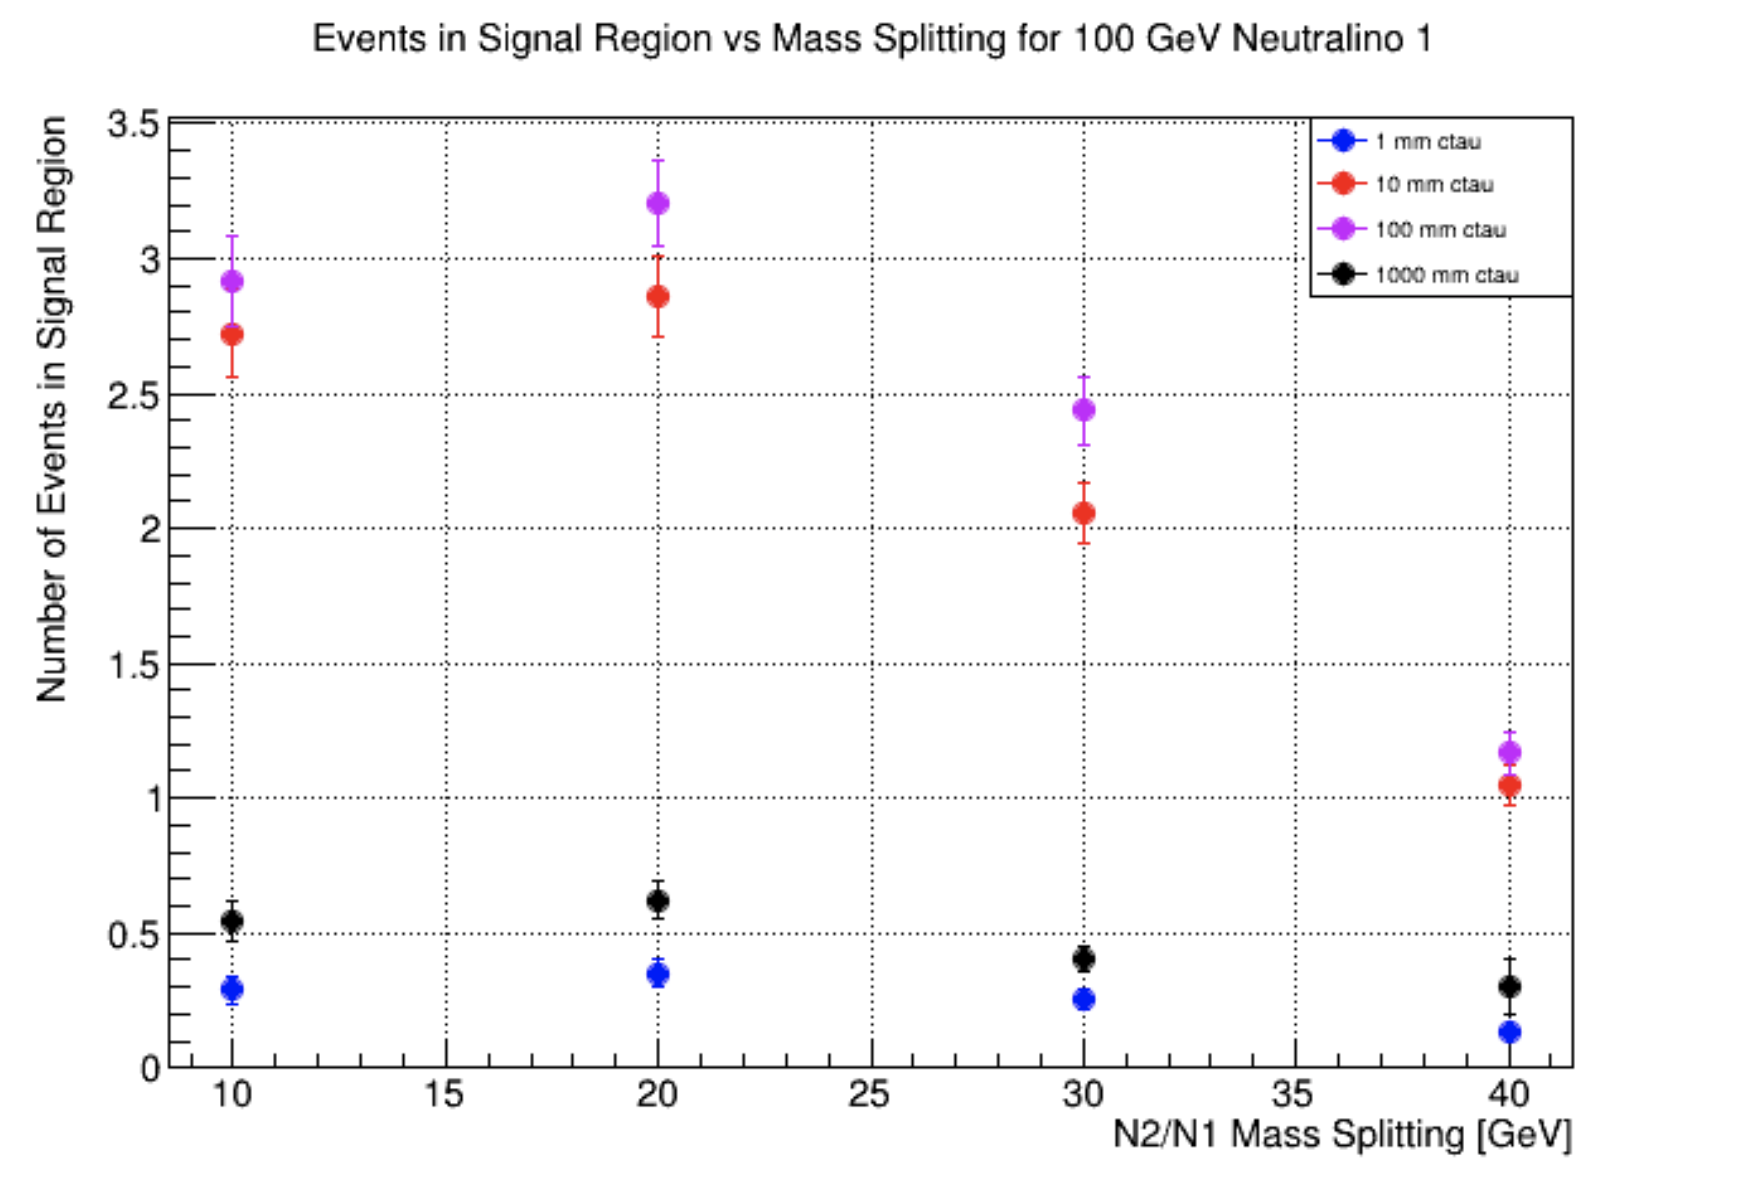
\includegraphics[width=.8\linewidth]{100GeV.png}  
  \caption{100 GeV $\chi_{1}^{0}$}
  \label{fig:sub-first19}
\end{subfigure}
\begin{subfigure}{.5\textwidth}
  \centering
  % include second image
  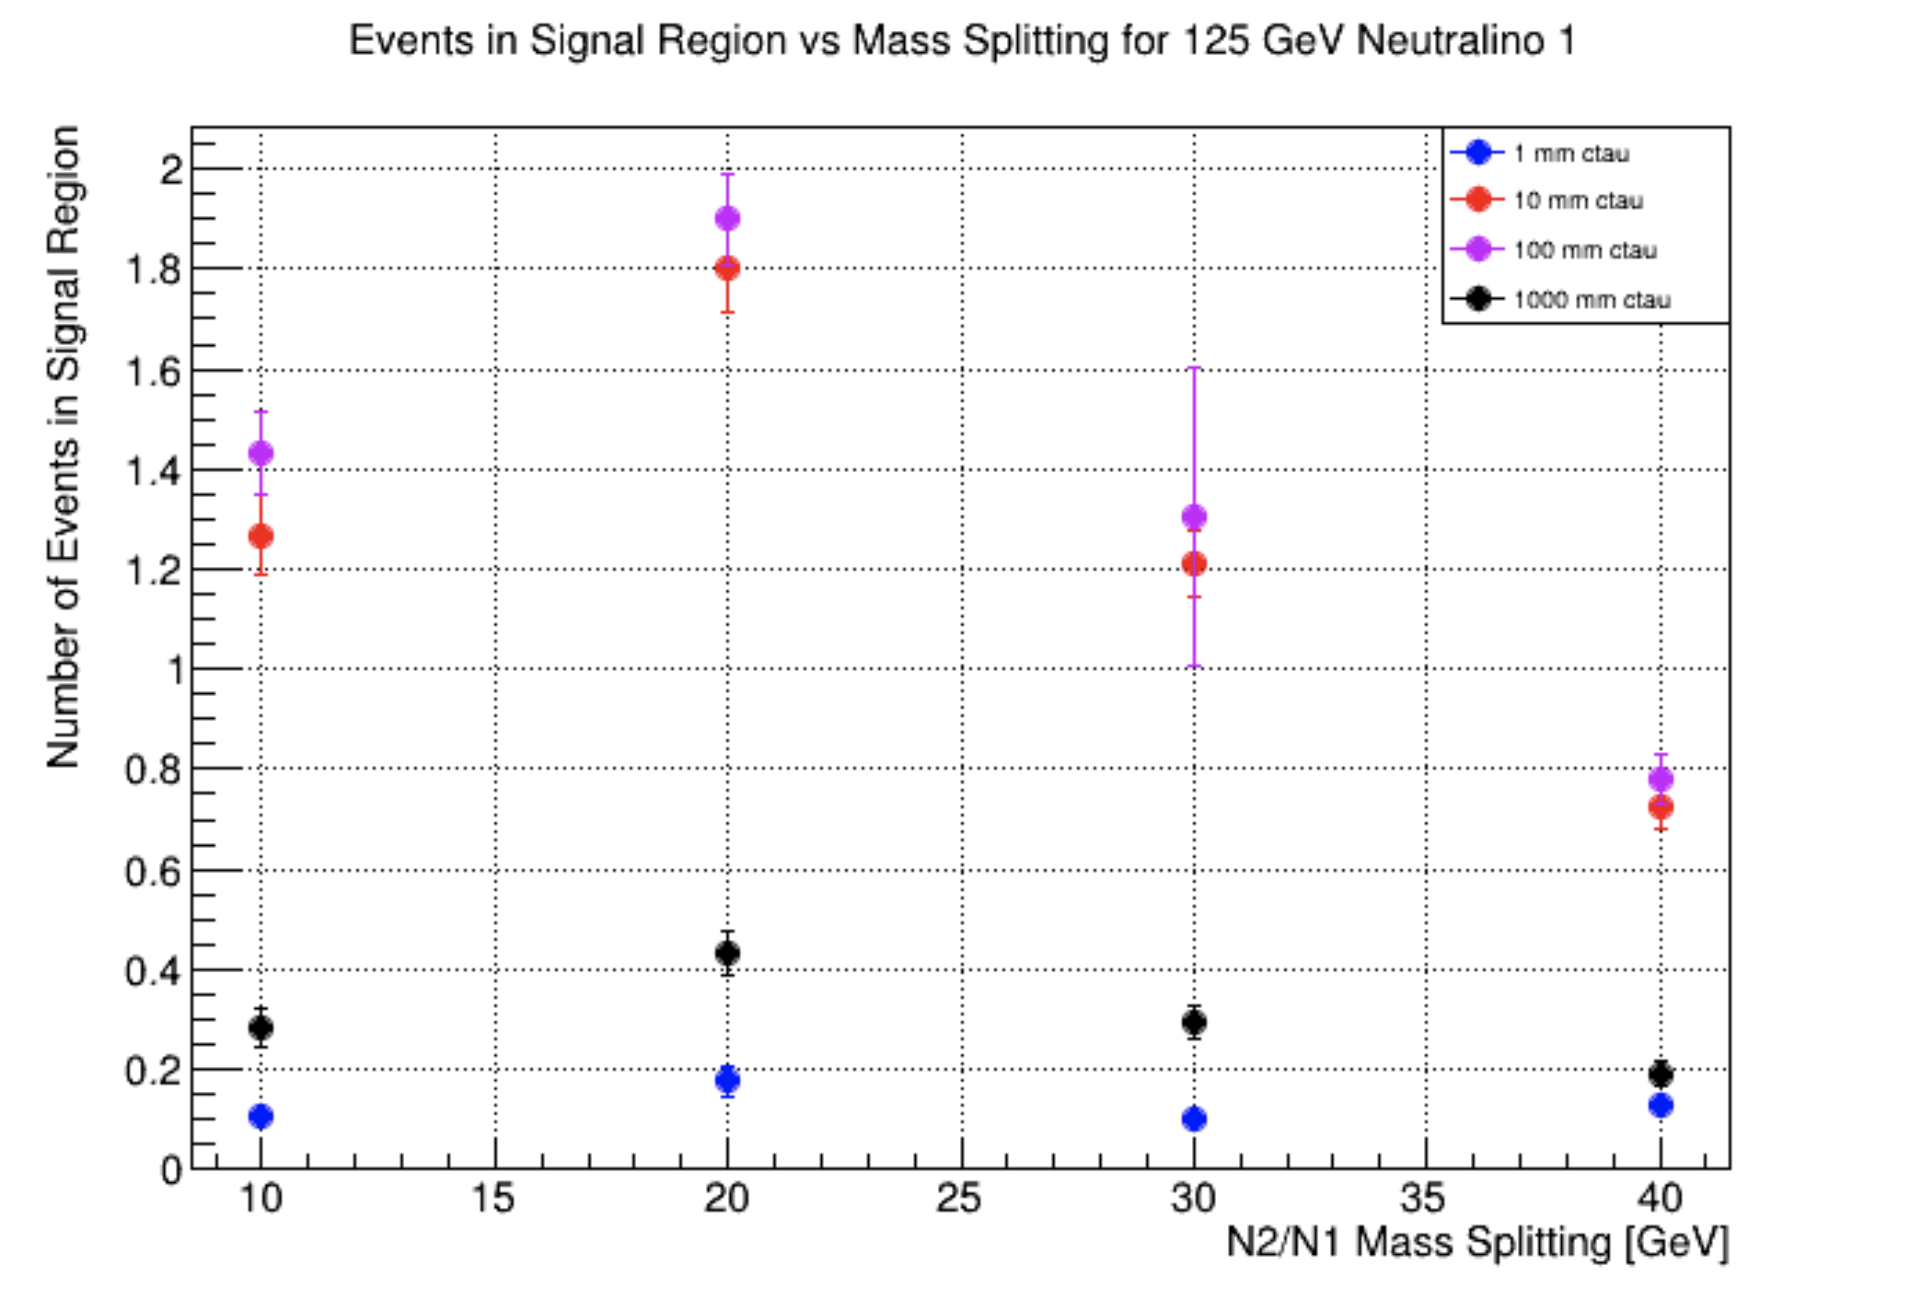
\includegraphics[width=.8\linewidth]{125GeV.png}  
  \caption{125 GeV $\chi_{1}^{0}$}
  \label{fig:sub-second19}
\end{subfigure}
\caption{Events in Signal Region for fixed $\chi_{1}^{0}$ mass in Higgsino Samples}
\label{fig:19}
\end{figure}

\begin{figure} [H]
\begin{subfigure}{.5\textwidth}
  \centering
  % include first image
  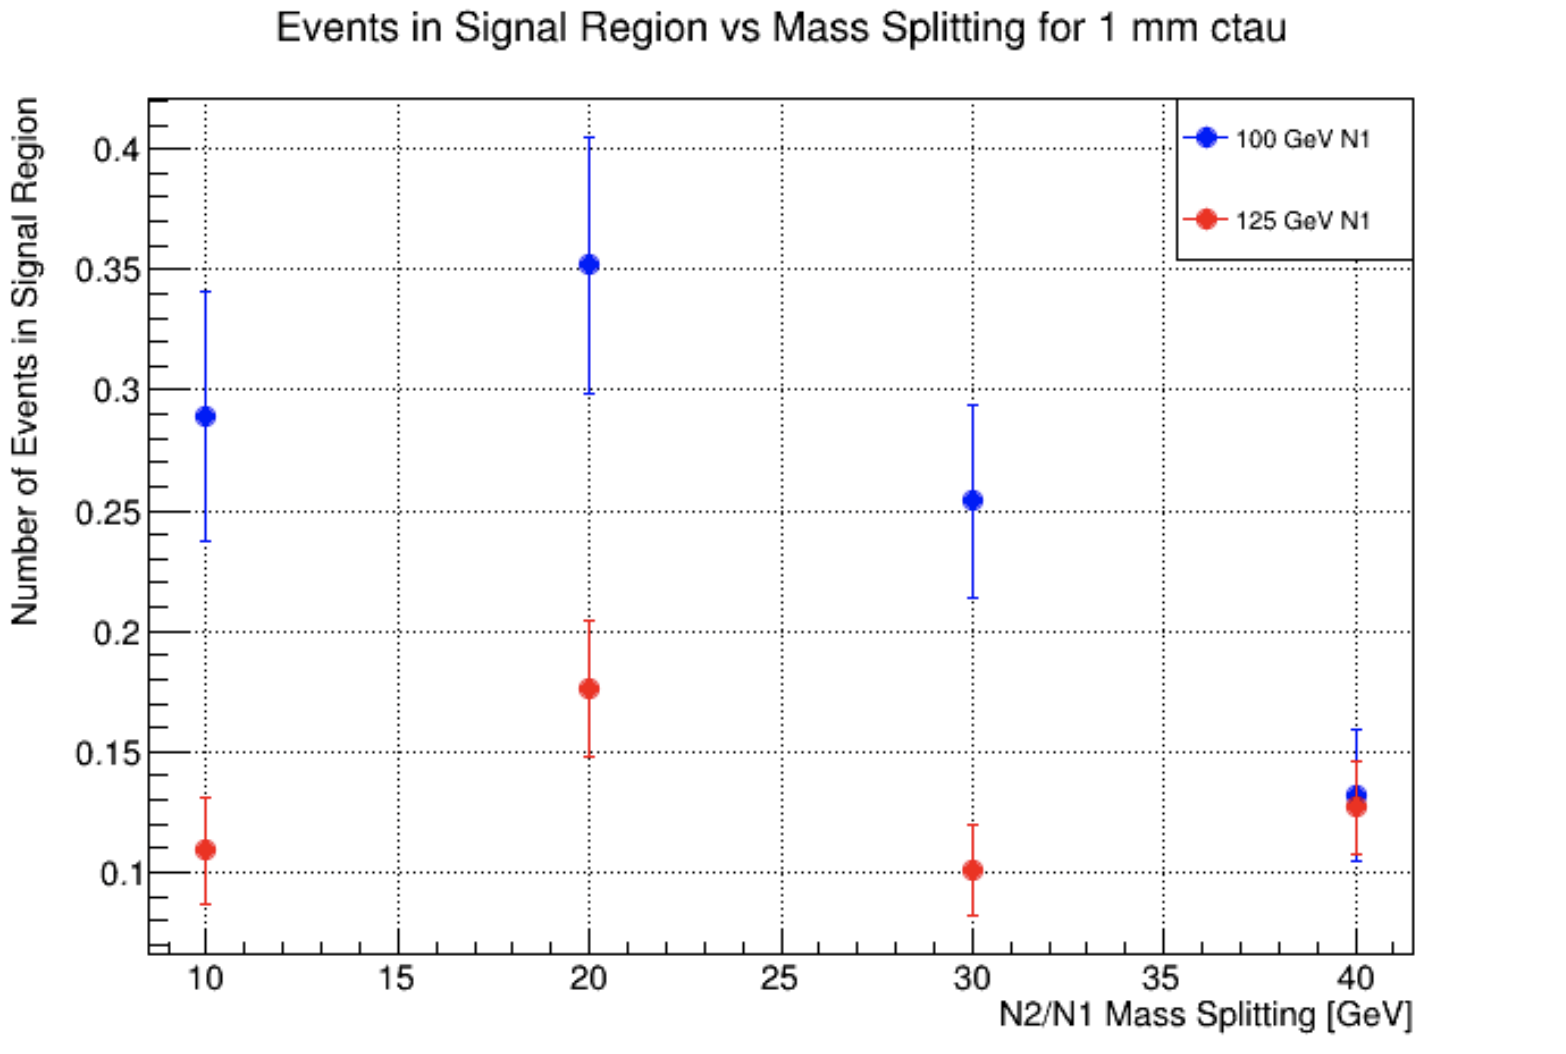
\includegraphics[width=.8\linewidth]{1mm.png}  
  \caption{1 mm ctau}
  \label{fig:sub-first18}
\end{subfigure}
\begin{subfigure}{.5\textwidth}
  \centering
  % include second image
  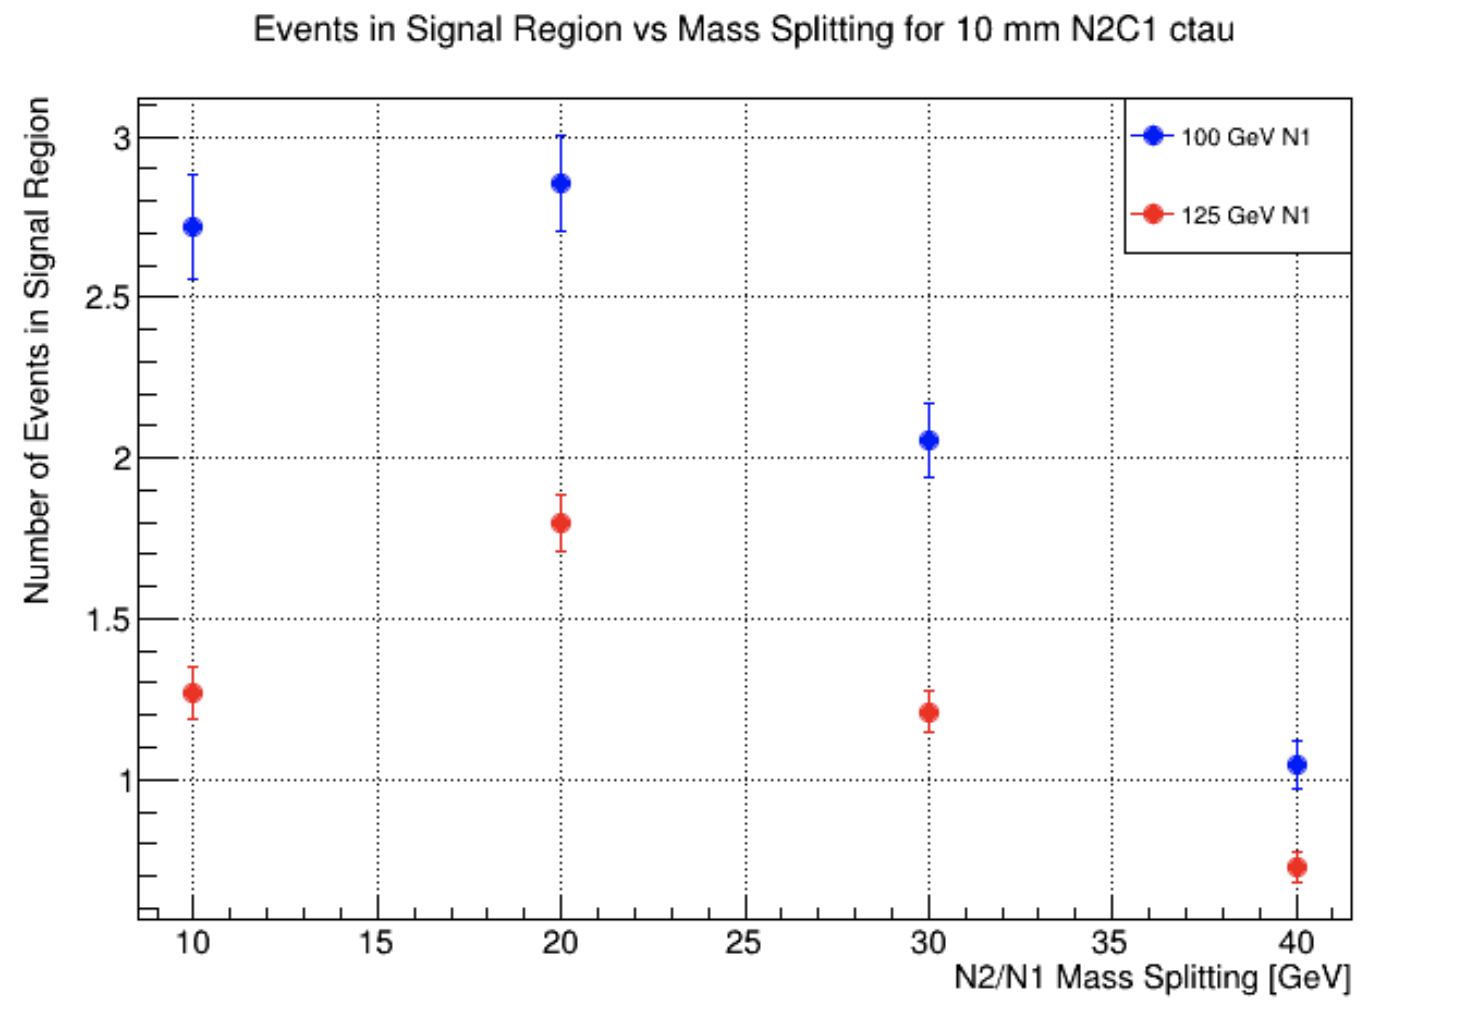
\includegraphics[width=.8\linewidth]{10mm.png}  
  \caption{10 mm ctau}
  \label{fig:sub-second18}
\end{subfigure}
\begin{subfigure}{.5\textwidth}
  \centering
  % include third image
  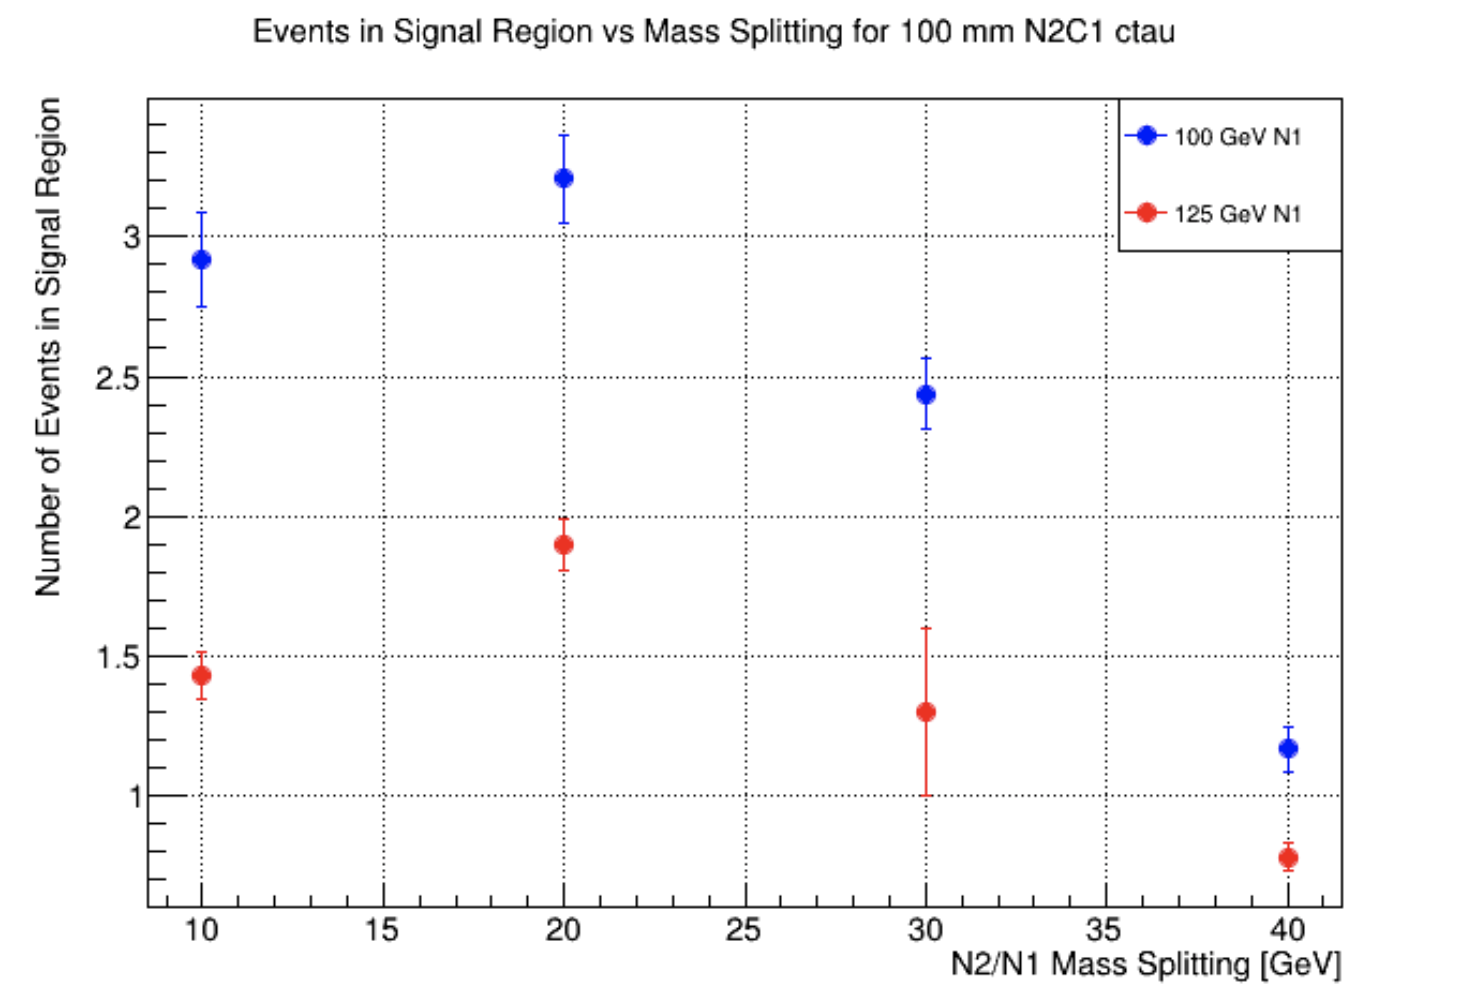
\includegraphics[width=.8\linewidth]{100mm.png}  
  \caption{100 mm ctau}
  \label{fig:sub-third18}
\end{subfigure}
\begin{subfigure}{.5\textwidth}
  \centering
  % include fourth image
  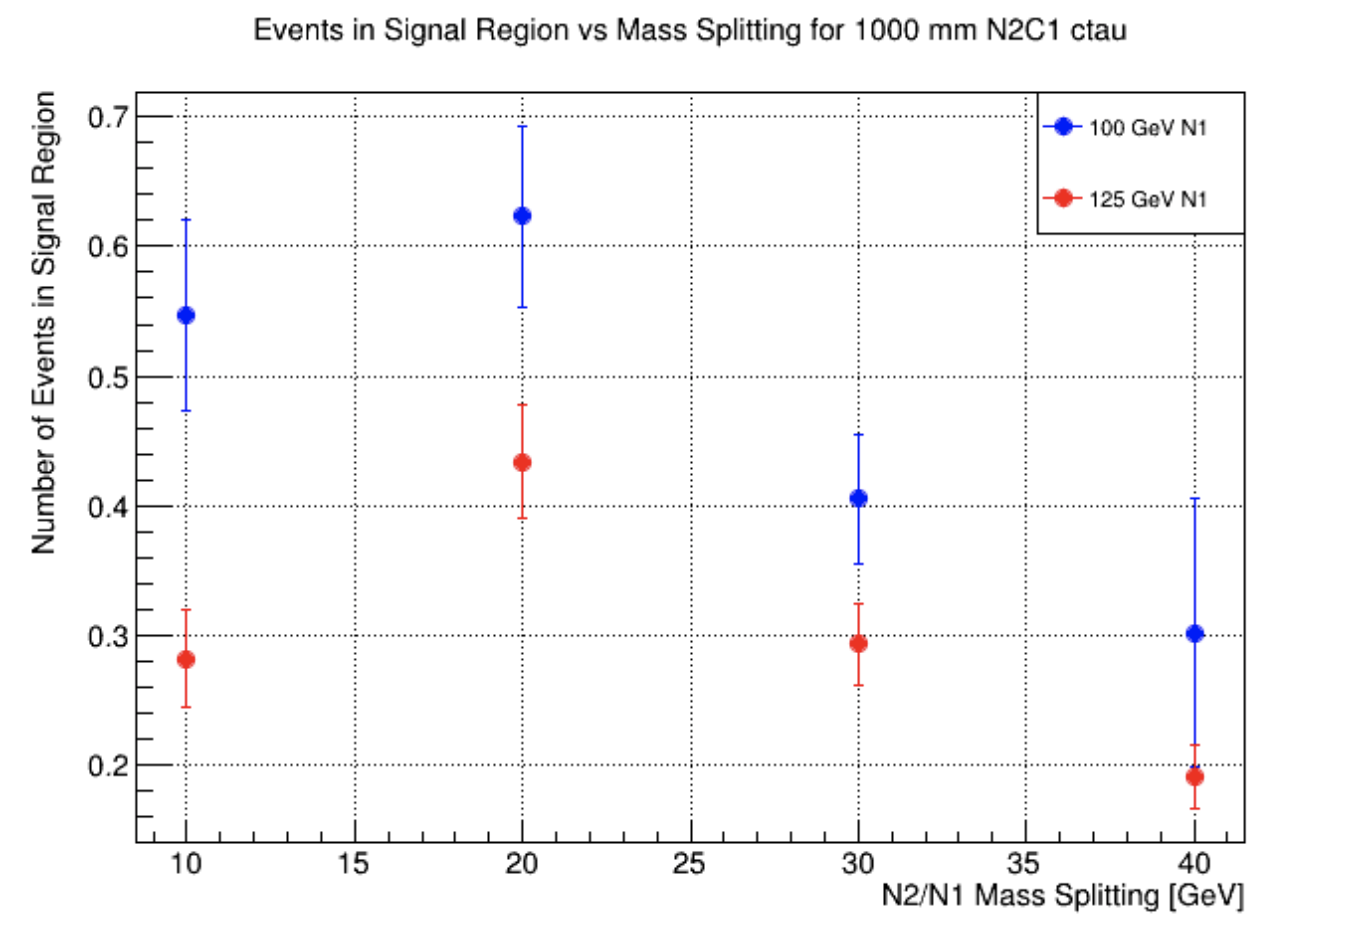
\includegraphics[width=.8\linewidth]{1000mm.png}  
  \caption{1000 mm ctau}
  \label{fig:sub-fourth18}
\end{subfigure}
\caption{Events in Signal Region for fixed ctau in Higgsino Samples}
\label{fig:20}
\end{figure}
\par
For the Wino/Bino case, figure~\ref{fig:21} shows the events in the signal region for a given $\chi_{2}^{0}$ mass, while figure~\ref{fig:22} shows the events for a fixed ctau.
\par
\begin{figure} [H]
\begin{subfigure}{.5\textwidth}
  \centering
  % include first image
  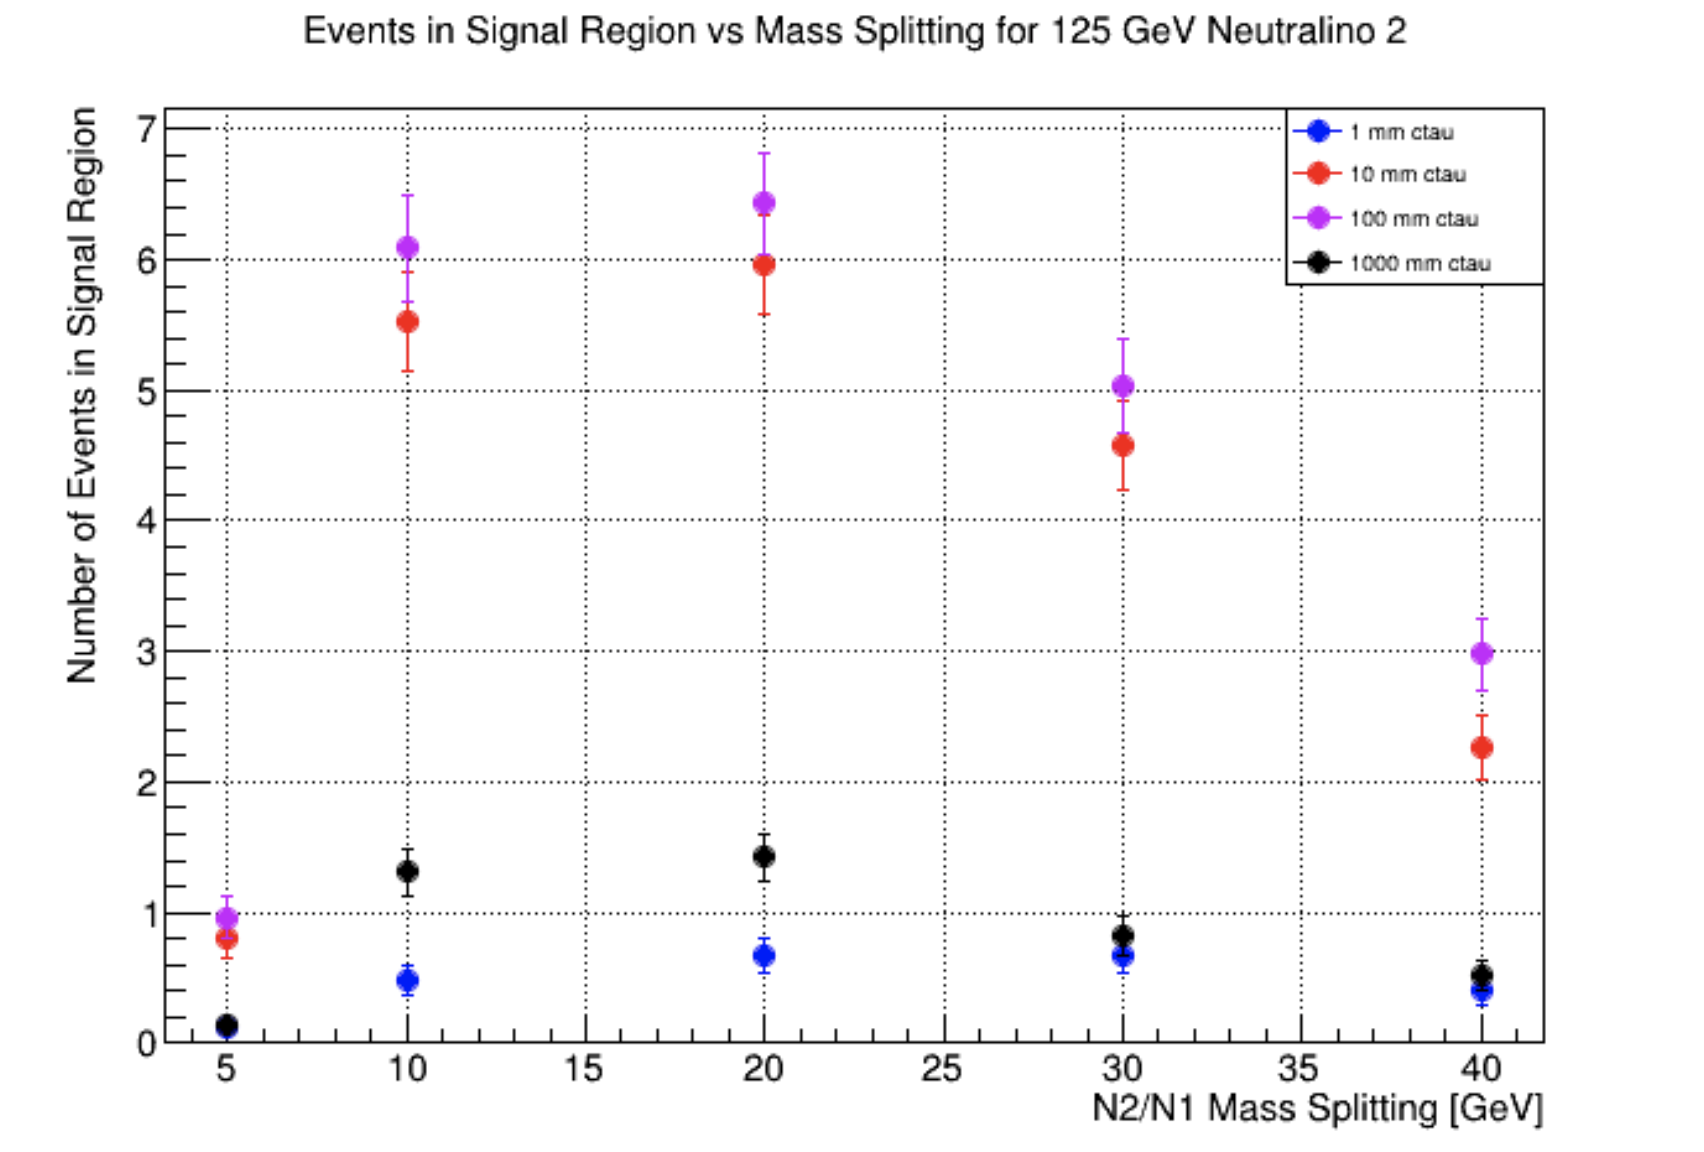
\includegraphics[width=.8\linewidth]{125GeVWino.png}  
  \caption{125 GeV $\chi_{2}^{0}$}
  \label{fig:sub-first19}
\end{subfigure}
\begin{subfigure}{.5\textwidth}
  \centering
  % include second image
  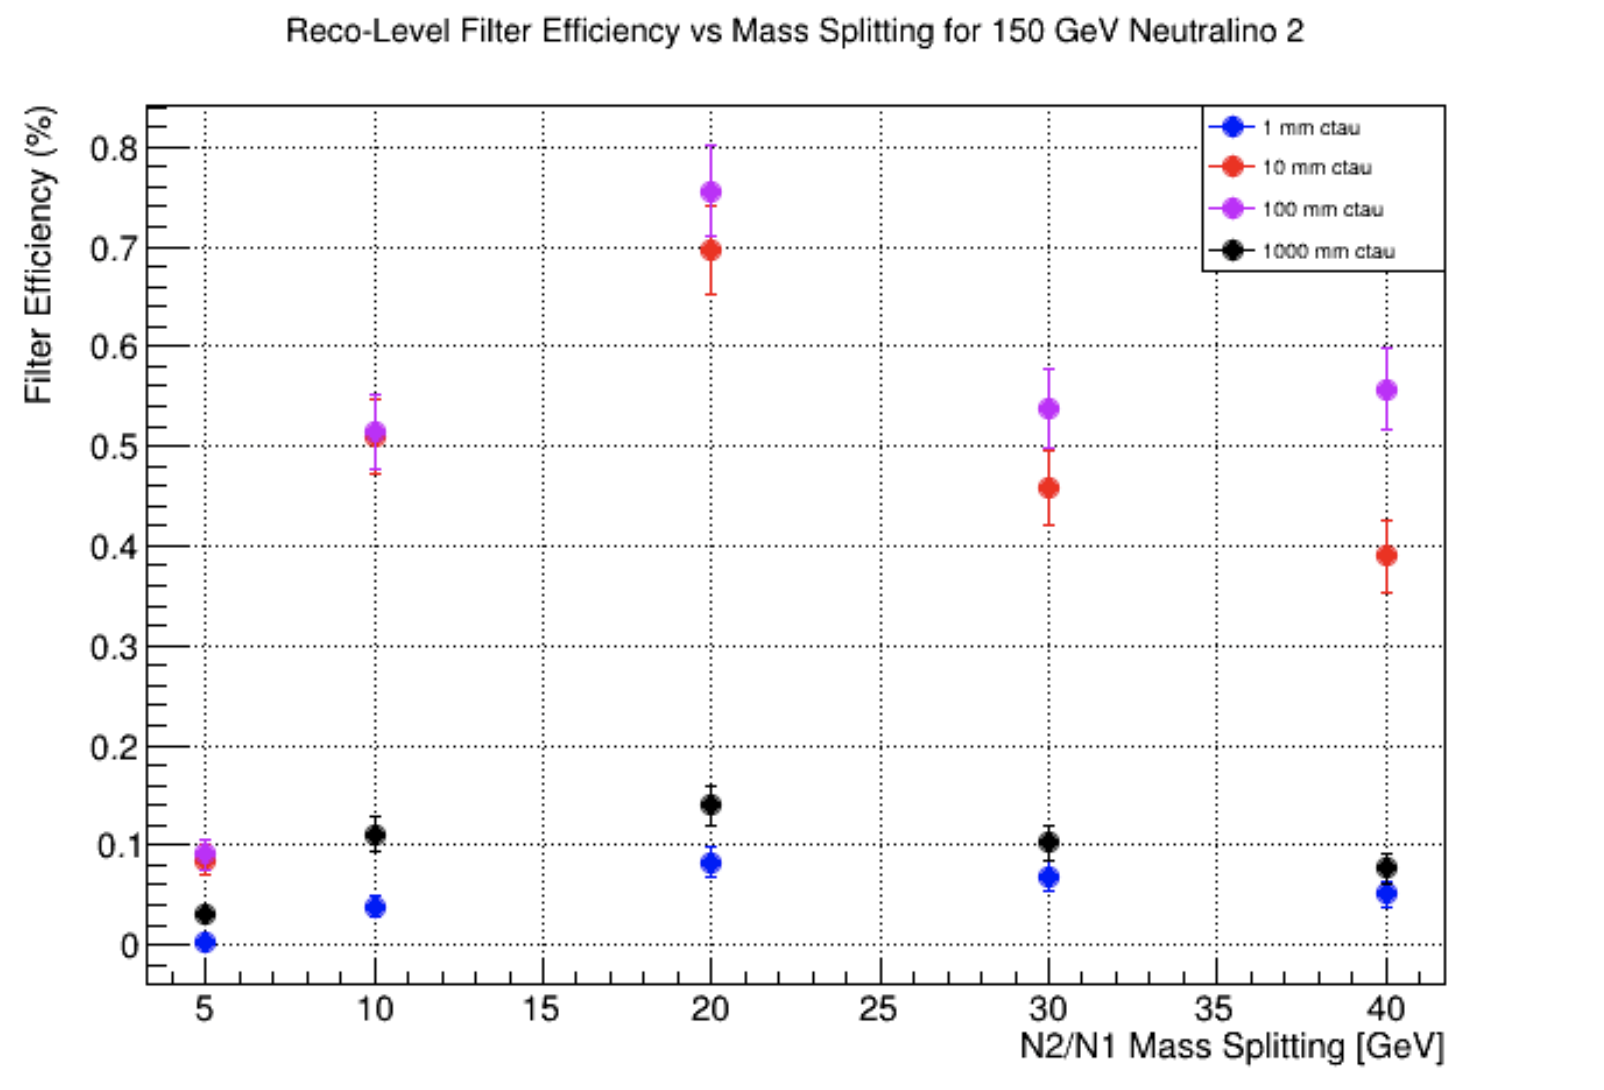
\includegraphics[width=.8\linewidth]{150GeVWino.png}  
  \caption{$\chi_{2}^{0}$ Wino/Bino}
  \label{fig:sub-second19}
\end{subfigure}
\caption{Events in Signal Region for fixed $\chi_{2}^{0}$ mass in Wino/Bino Samples}
\label{fig:21}
\end{figure}

\begin{figure} [H]
\begin{subfigure}{.5\textwidth}
  \centering
  % include first image
  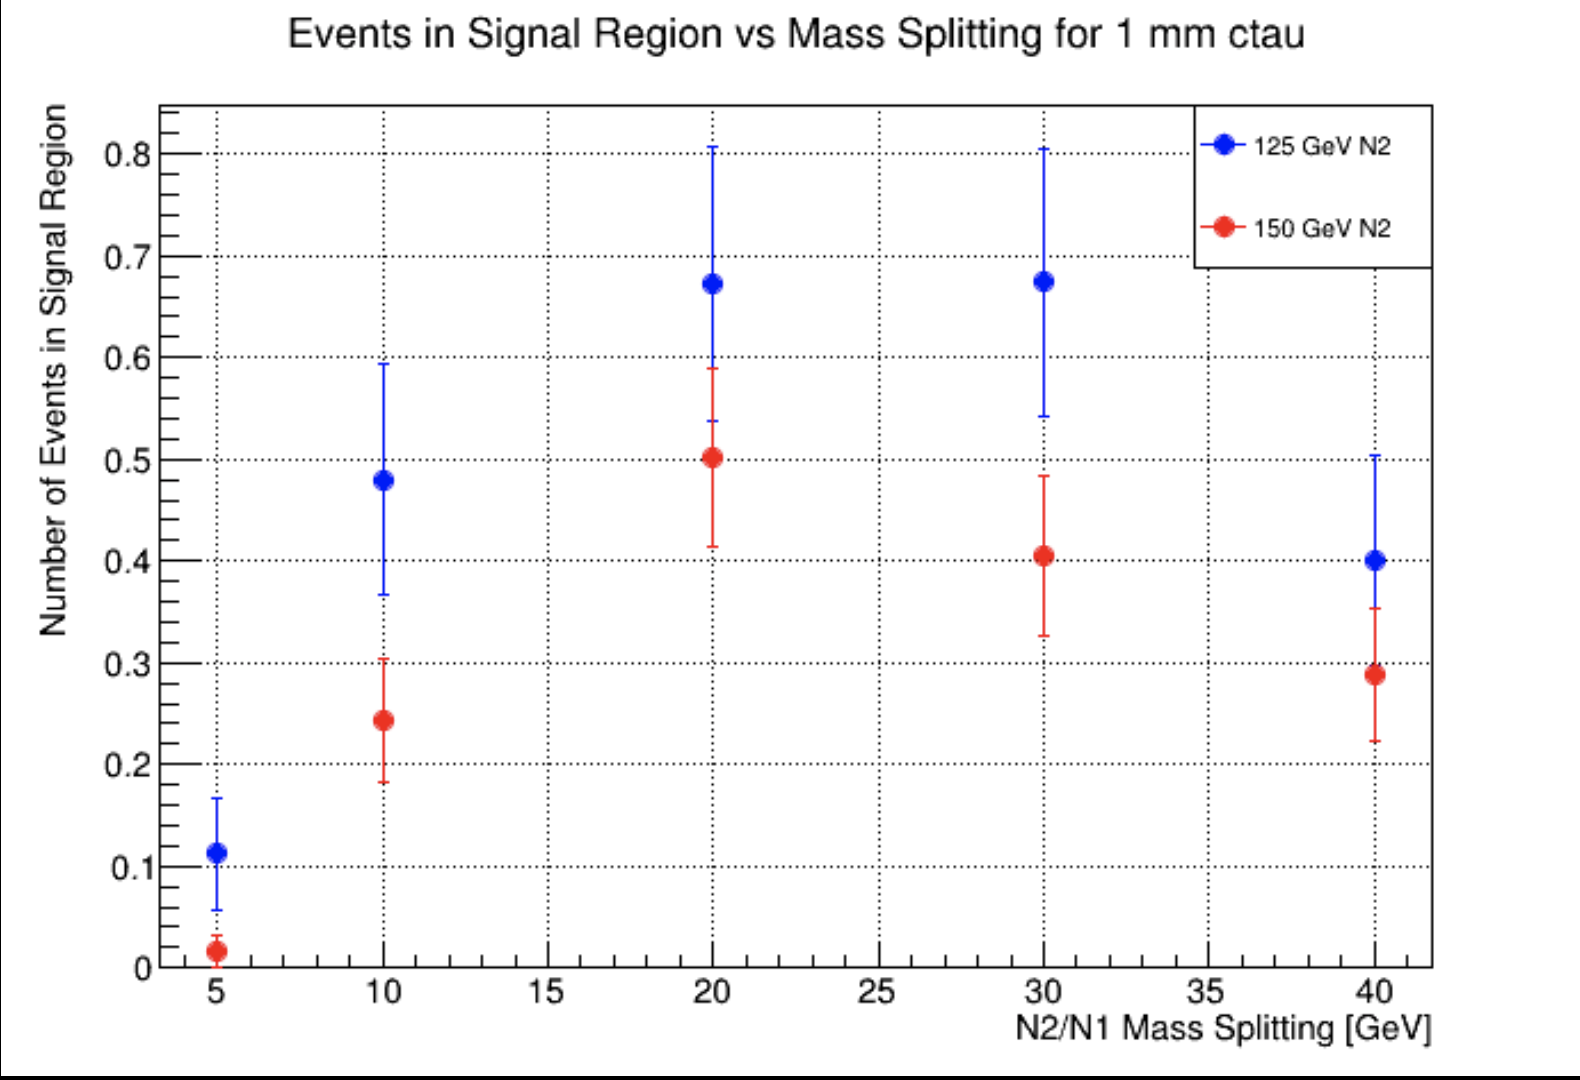
\includegraphics[width=.8\linewidth]{1mmWino.png}  
  \caption{1 mm ctau}
  \label{fig:sub-first18}
\end{subfigure}
\begin{subfigure}{.5\textwidth}
  \centering
  % include second image
  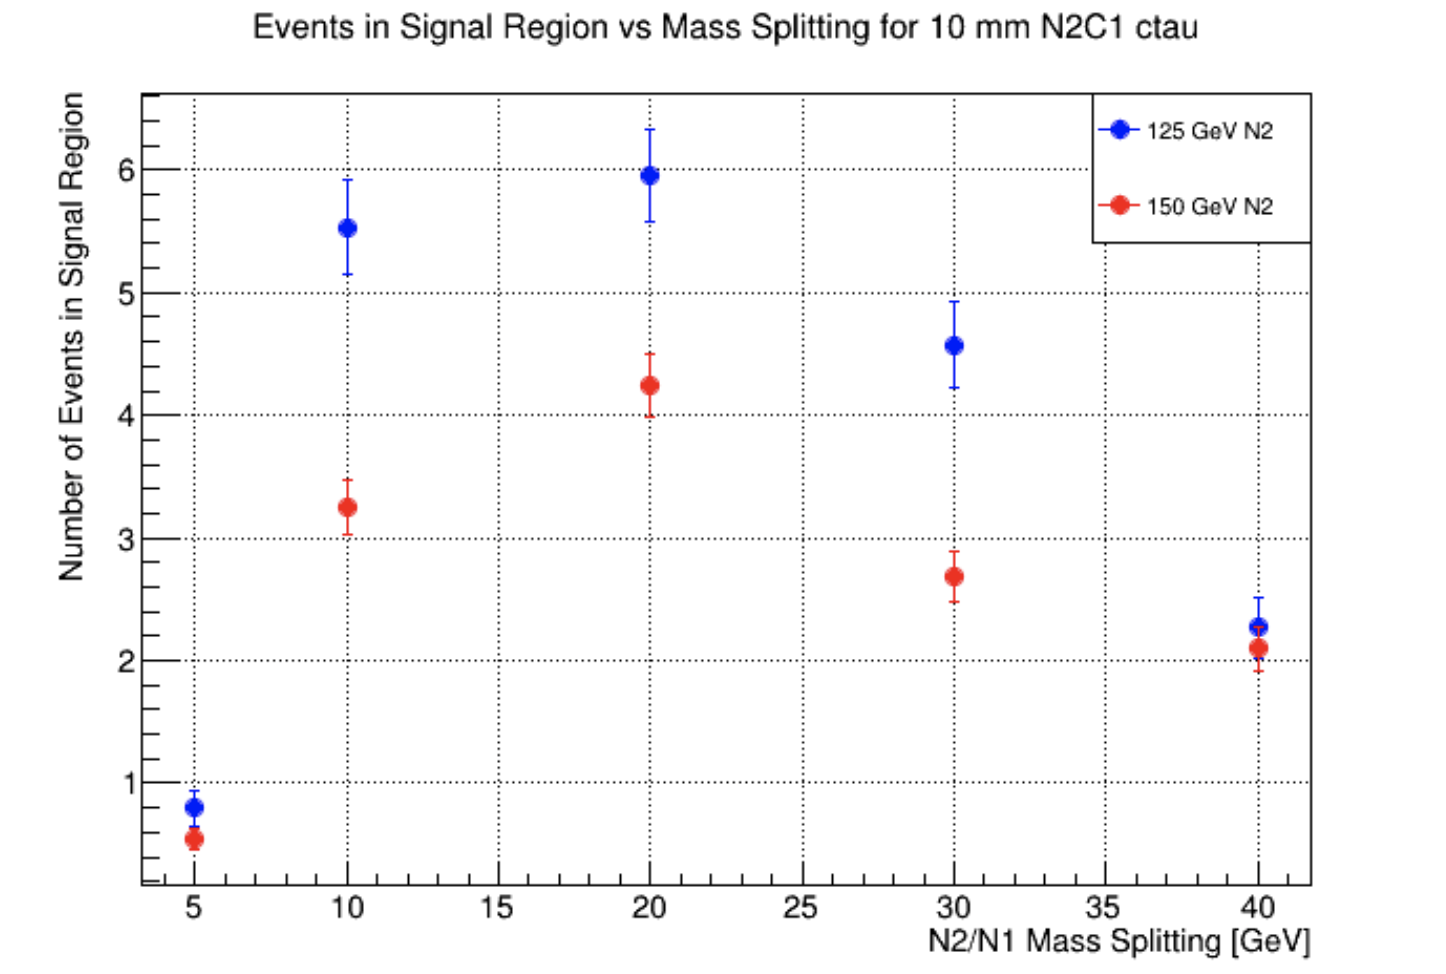
\includegraphics[width=.8\linewidth]{10mmWino.png}  
  \caption{10 mm ctau}
  \label{fig:sub-second18}
\end{subfigure}
\begin{subfigure}{.5\textwidth}
  \centering
  % include third image
  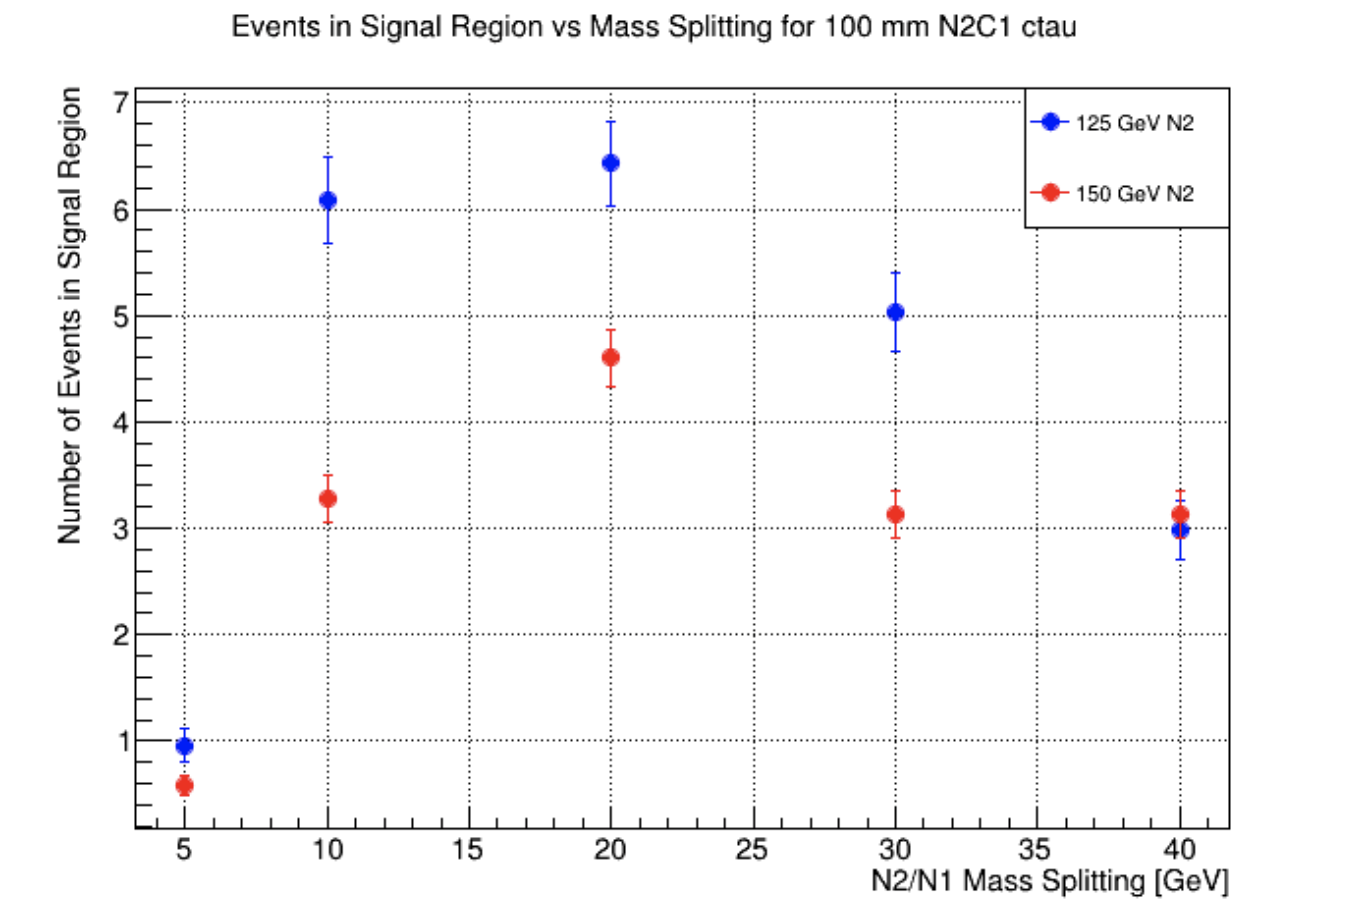
\includegraphics[width=.8\linewidth]{100mmWino.png}  
  \caption{100 mm ctau}
  \label{fig:sub-third18}
\end{subfigure}
\begin{subfigure}{.5\textwidth}
  \centering
  % include fourth image
  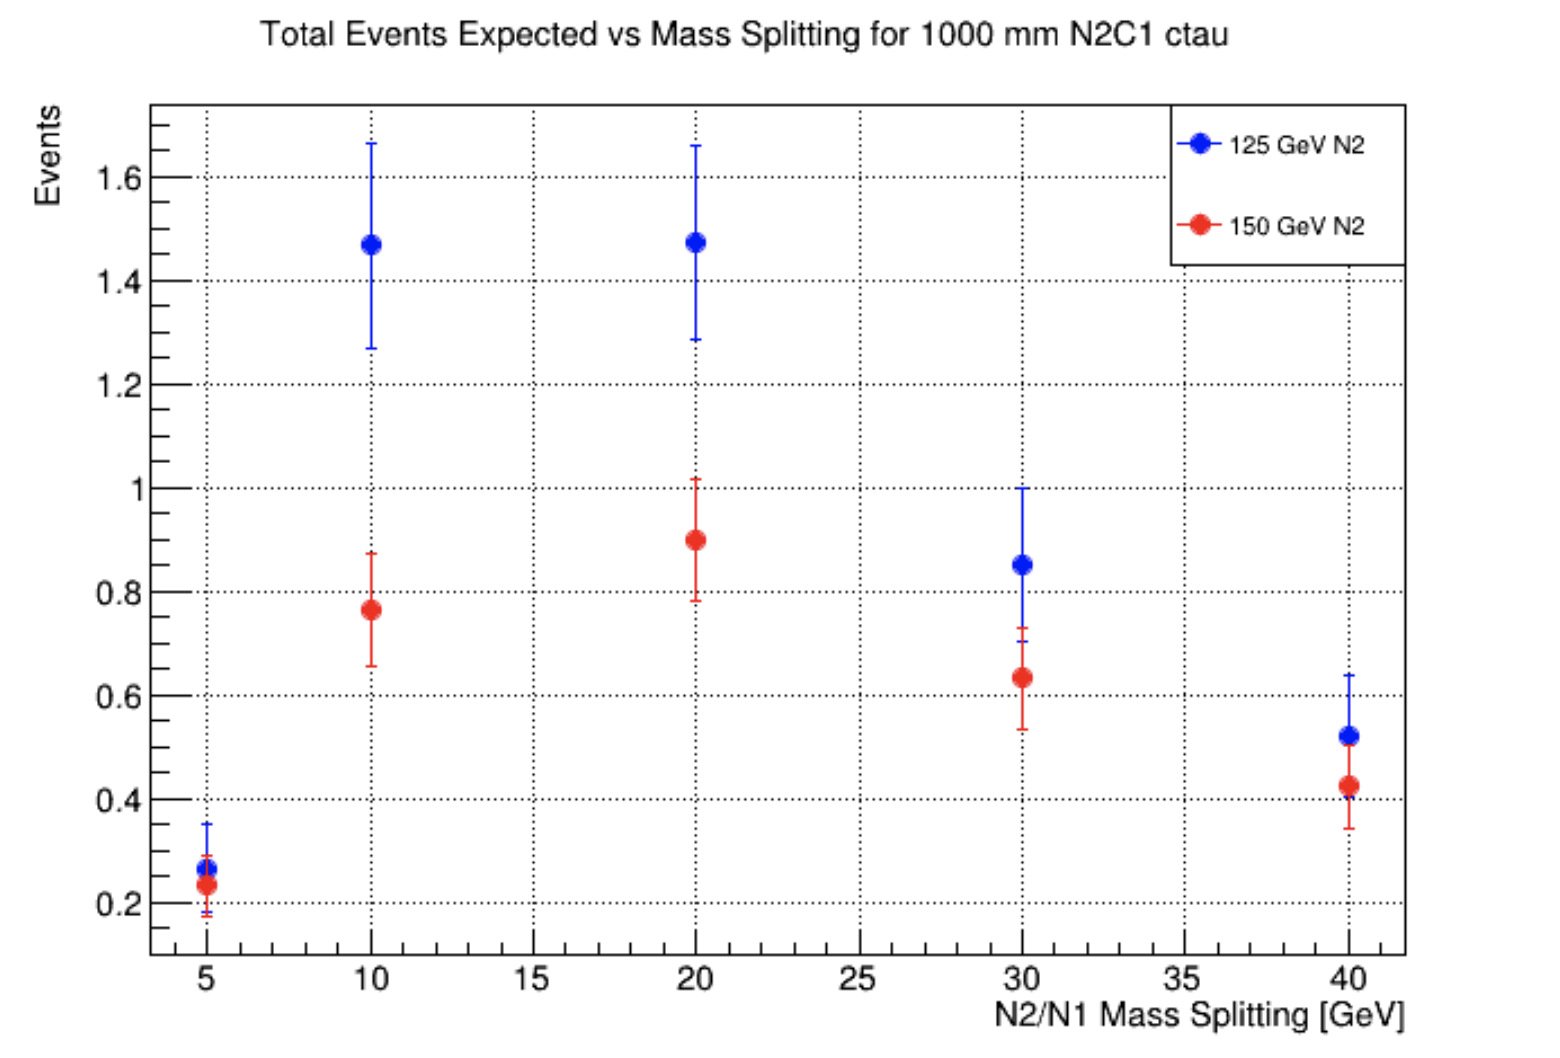
\includegraphics[width=.8\linewidth]{1000mmWino.png}  
  \caption{1000 mm ctau}
  \label{fig:sub-fourth18}
\end{subfigure}
\caption{Events in Signal Region for fixed ctau in Wino/Bino Samples}
\label{fig:22}
\end{figure}
\par
Since there is no background in our signal region, we expect to be sensitive to effectively any signal. Therefore, though we haven't found more than 6-7 events for a given mass configuration/lifetime combination, we should be sensitive to the signal if it does represent an existing phenomenon. However, in both the Higgsino and Wino/Bino models, we expect the most events at small neutralino masses with a mass splitting of about 10-20 GeV. At small mass splittings, a larger portion of events have a dimuon mass less than 3 GeV and therefore do not lie in the signal region, while at large mass splitting and larger neutralino masses in general, the initial theoretical cross-section is smaller, so fewer events are expected regardless of cuts. Earlier, we conclude that the efficiency of generator-level cuts is largely constant, regardless of the mass configuration of the sample. We measured the efficiency of the reconstruction-level cuts for each produced sample as well, and produced a similar set of plots as figures 20-23. The reco-level efficiency is defined as:
\[\epsilon_{r} = \frac{\sigma_{r}}{\sigma_{g}}\]
with a corresponding error of [15]:
\[\Delta\epsilon_{r} = \sqrt{\frac{\epsilon_{r}(1-\epsilon_{r})}{\text{Events in nTuple}}}\]
We include the number of events in the nTuple because the efficiency error depends on the number of unweighted events. Note that this expression for $\Delta\epsilon_{r}$ breaks down as $\epsilon_{r}$ $\rightarrow$ 0. We have very small efficiencies, so indeed our expression may not be entirely accurate, but it is sufficient for our analysis. Figure~\ref{fig:23} displays the reco efficiency for a given $\chi_{1}^{0}$ mass in the Higgsino case. Figure~\ref{fig:24} displays the number of events in the signal region for a fixed ctau.
\par
\begin{figure} [H]
\begin{subfigure}{.5\textwidth}
  \centering
  % include first image
  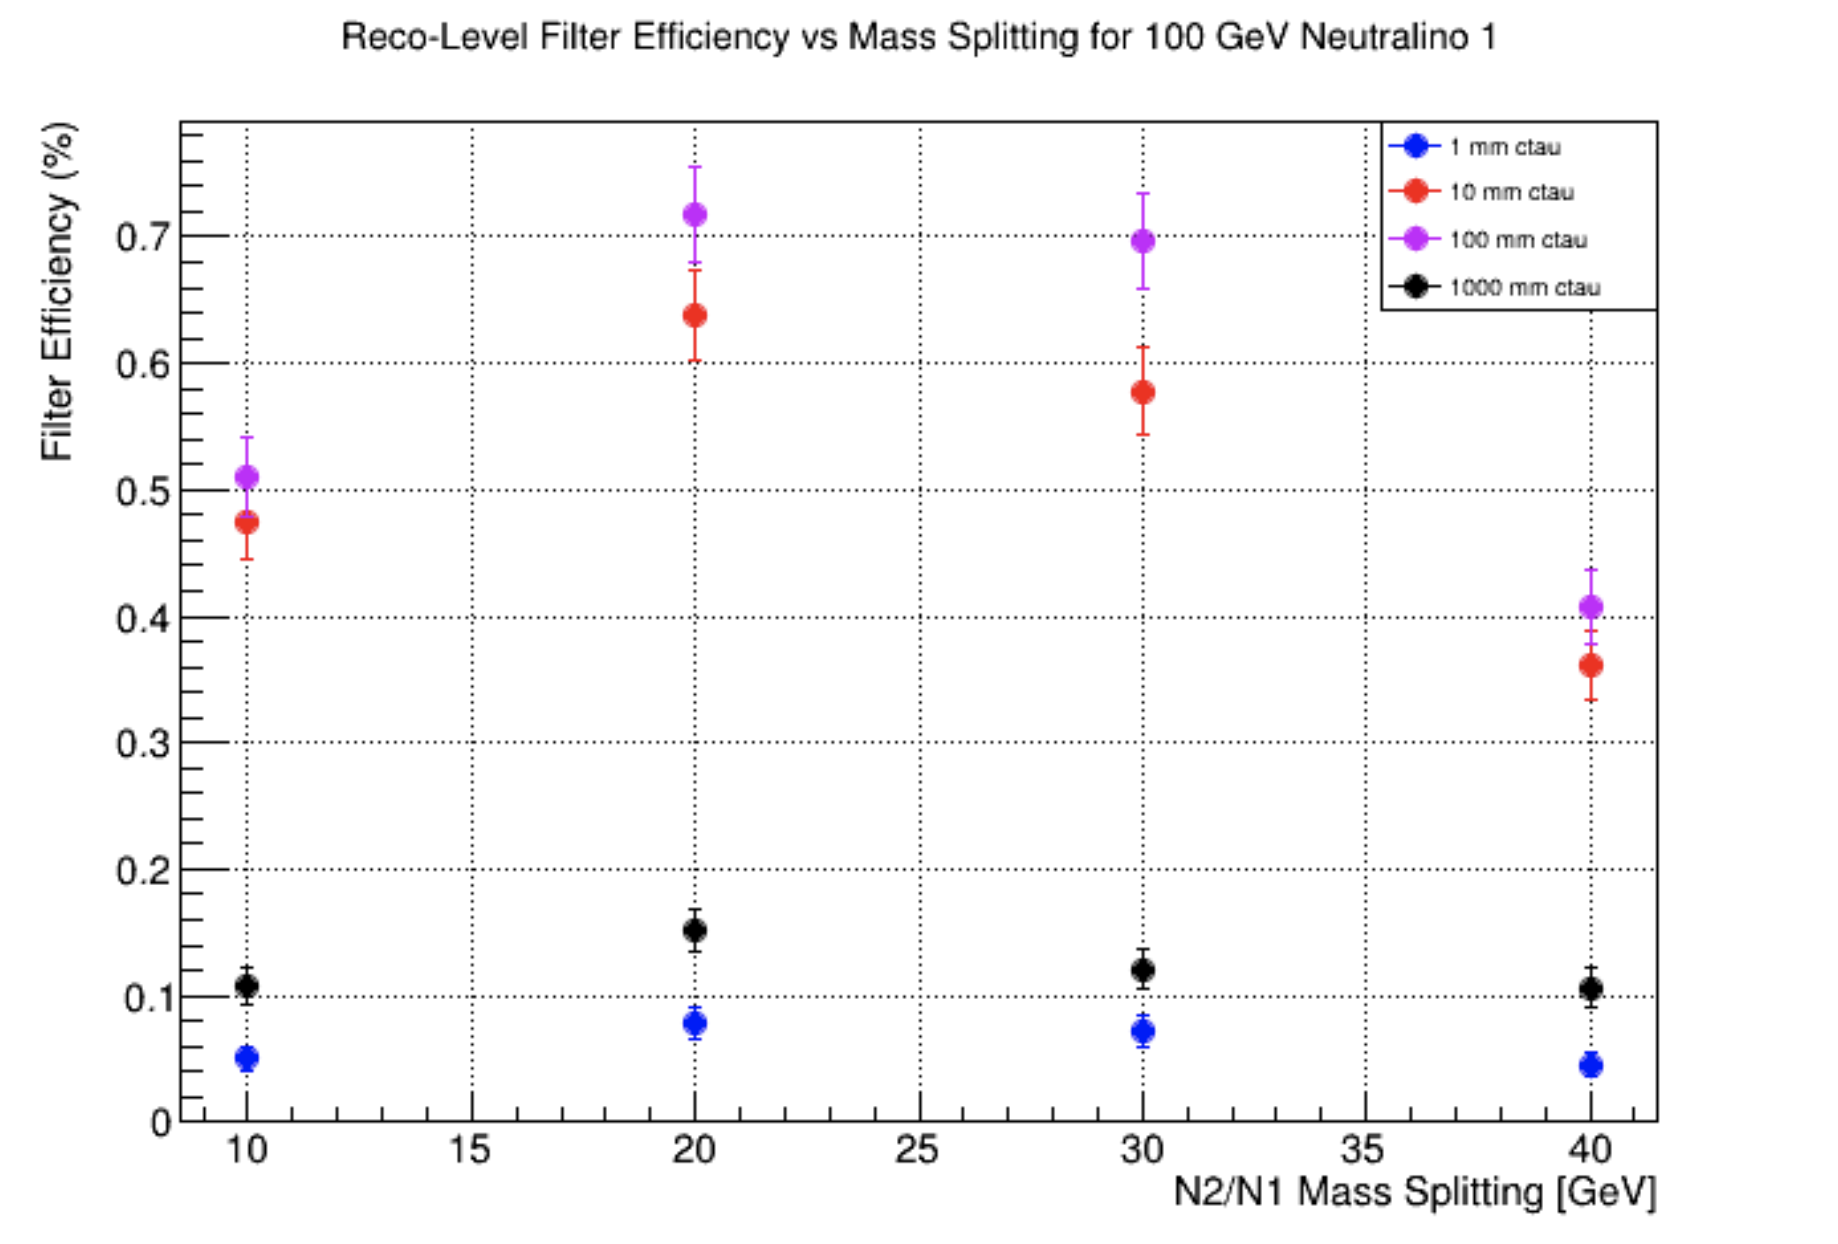
\includegraphics[width=.8\linewidth]{100GeVEff.png}  
  \caption{100 GeV $\chi_{1}^{0}$}
  \label{fig:sub-first19}
\end{subfigure}
\begin{subfigure}{.5\textwidth}
  \centering
  % include second image
  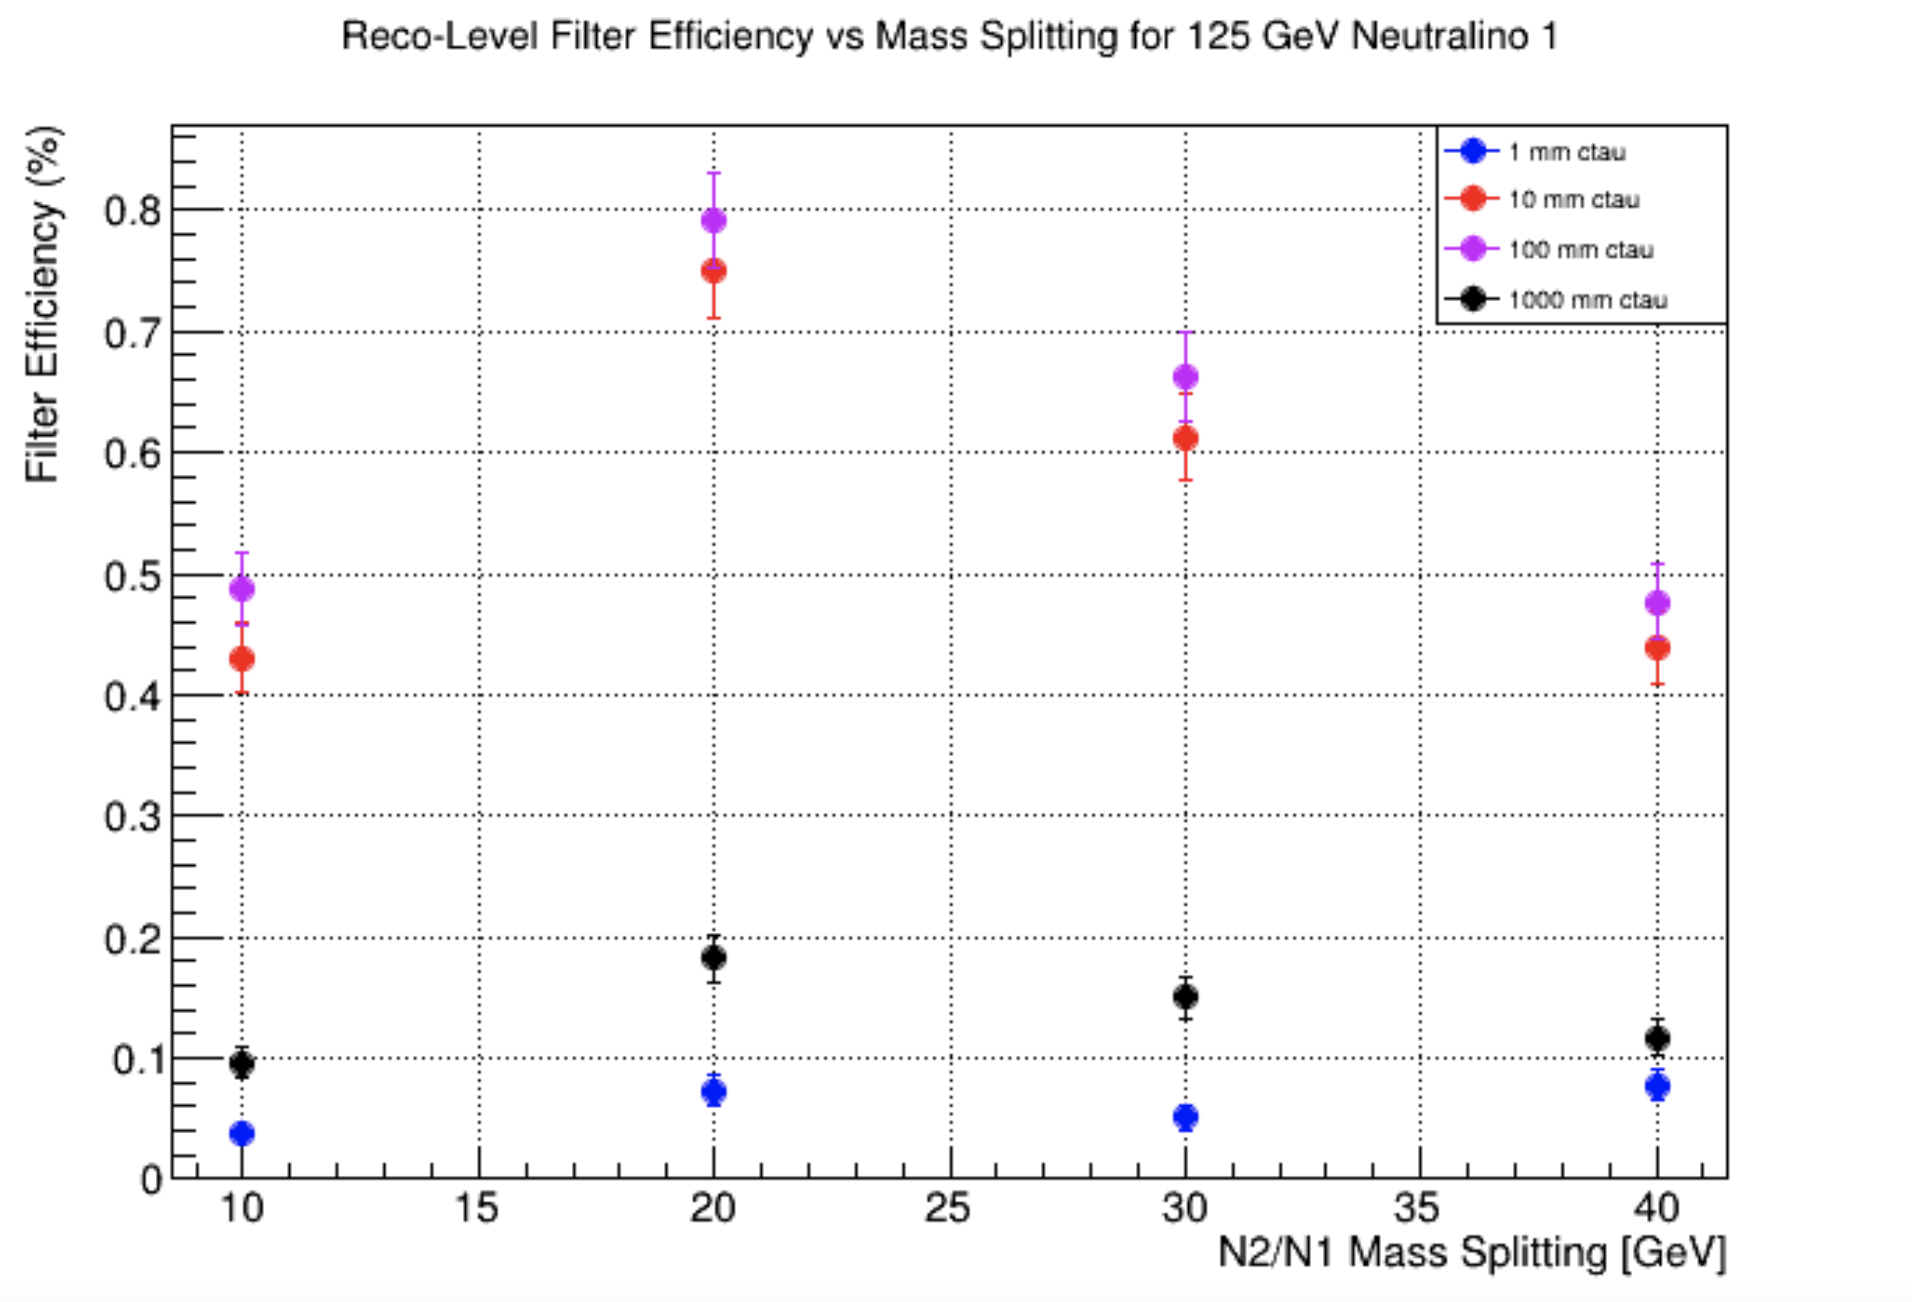
\includegraphics[width=.8\linewidth]{125GeVEff.png}  
  \caption{125 GeV $\chi_{1}^{0}$}
  \label{fig:sub-second19}
\end{subfigure}
\caption{Reco-Level Efficiency for fixed $\chi_{1}^{0}$ mass in Higgsino Samples}
\label{fig:23}
\end{figure}

\begin{figure} [H]
\begin{subfigure}{.5\textwidth}
  \centering
  % include first image
  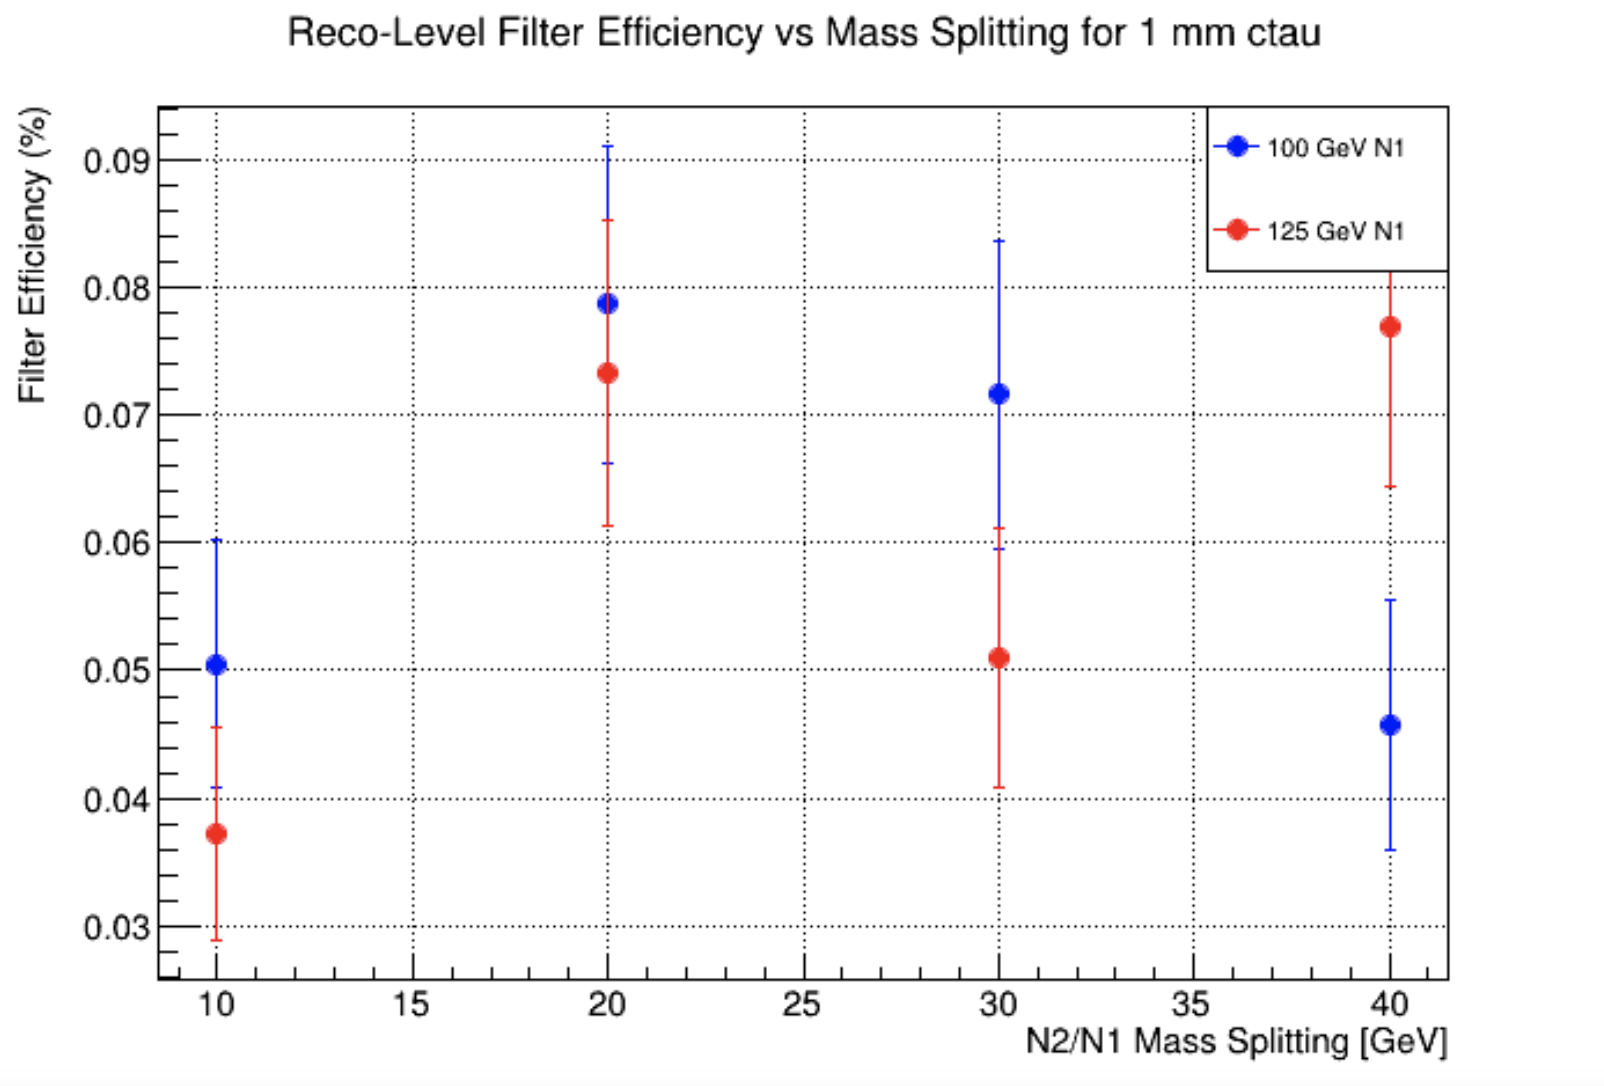
\includegraphics[width=.8\linewidth]{1mmEff.png}  
  \caption{1 mm ctau}
  \label{fig:sub-first18}
\end{subfigure}
\begin{subfigure}{.5\textwidth}
  \centering
  % include second image
  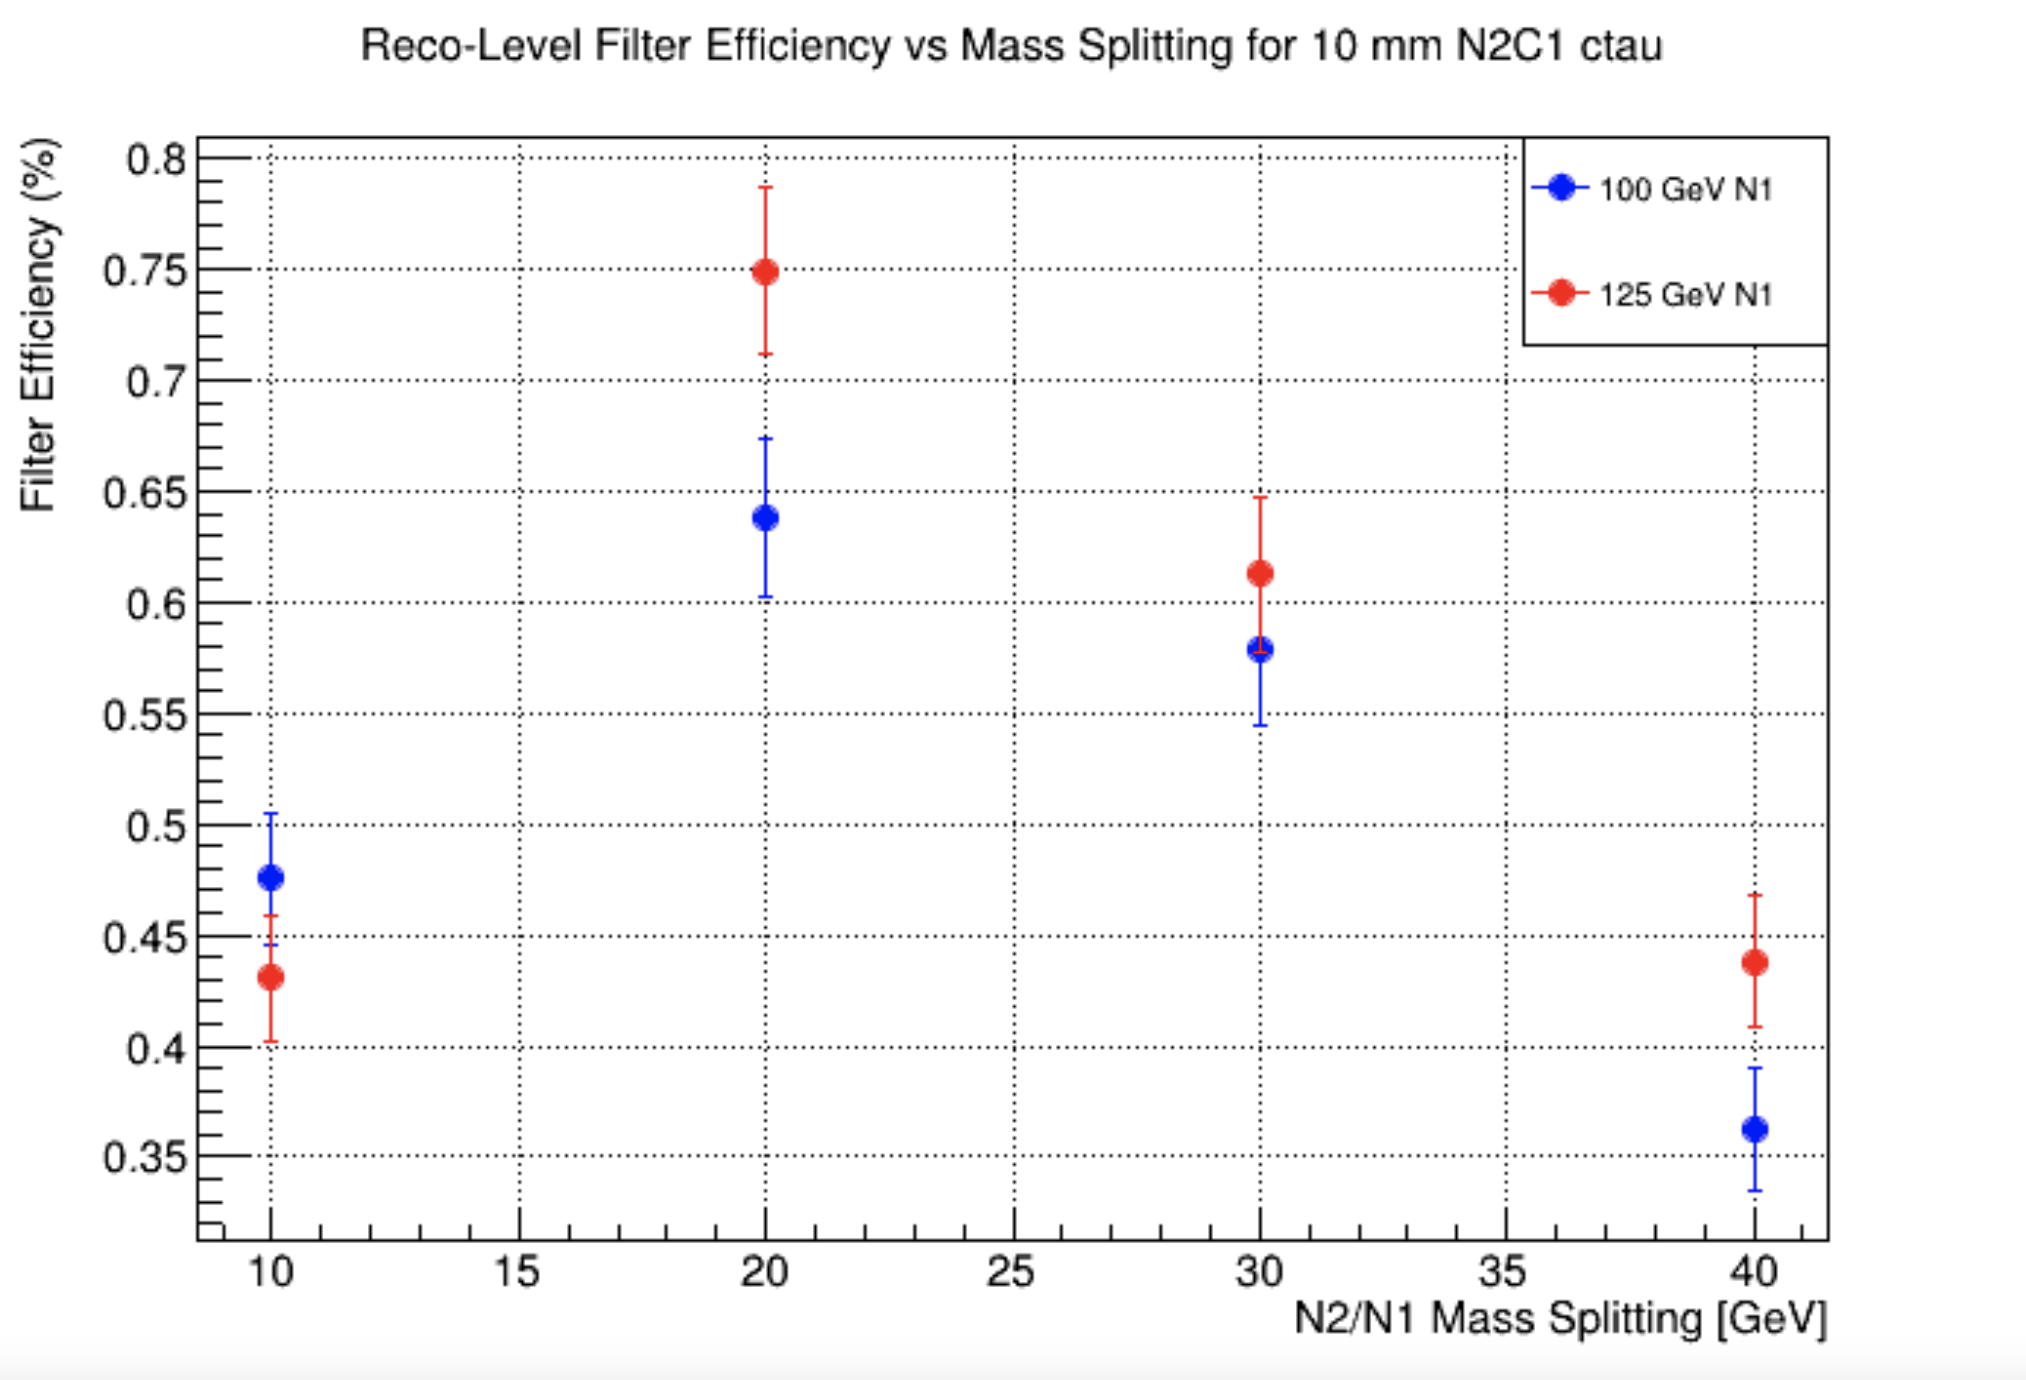
\includegraphics[width=.8\linewidth]{10mmEff.png}  
  \caption{10 mm ctau}
  \label{fig:sub-second18}
\end{subfigure}
\begin{subfigure}{.5\textwidth}
  \centering
  % include third image
  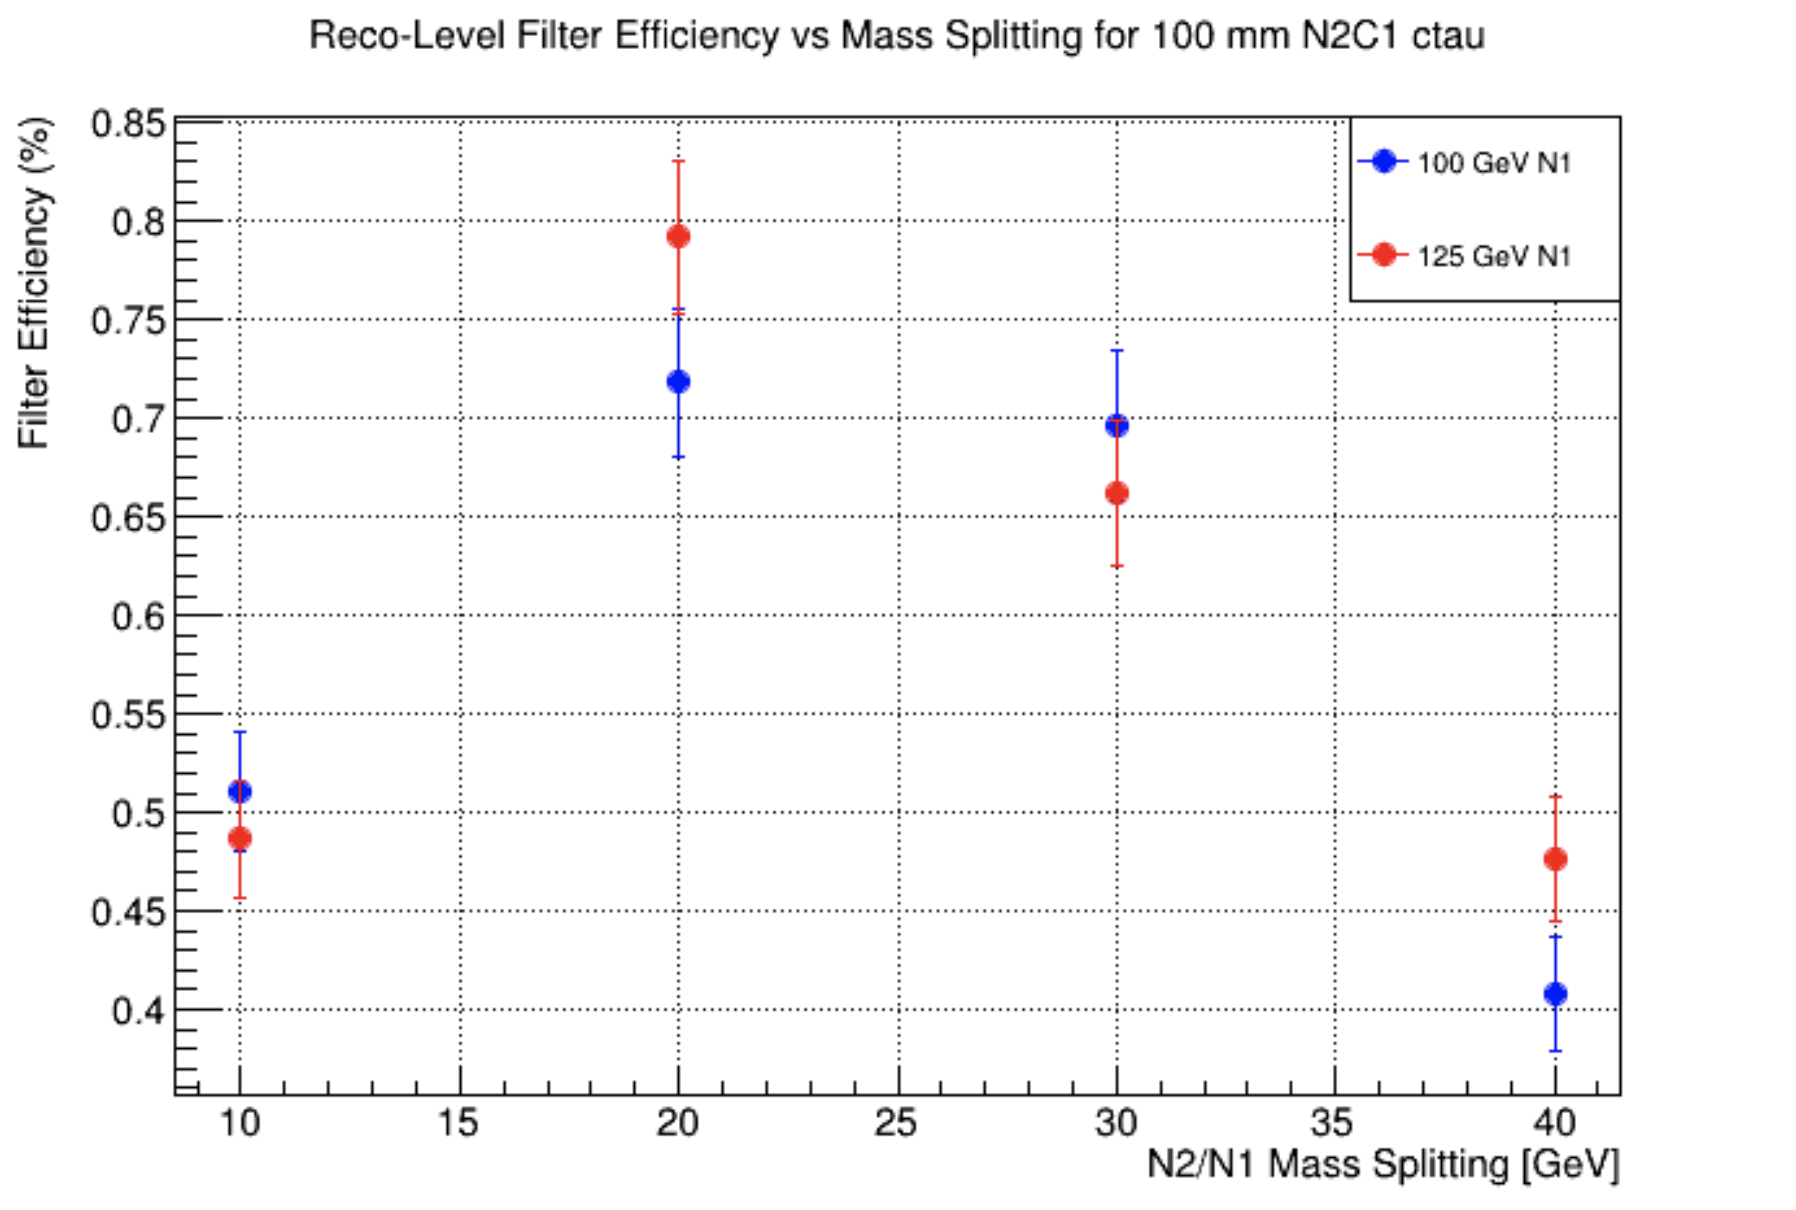
\includegraphics[width=.8\linewidth]{100mmEff.png}  
  \caption{100 mm ctau}
  \label{fig:sub-third18}
\end{subfigure}
\begin{subfigure}{.5\textwidth}
  \centering
  % include fourth image
  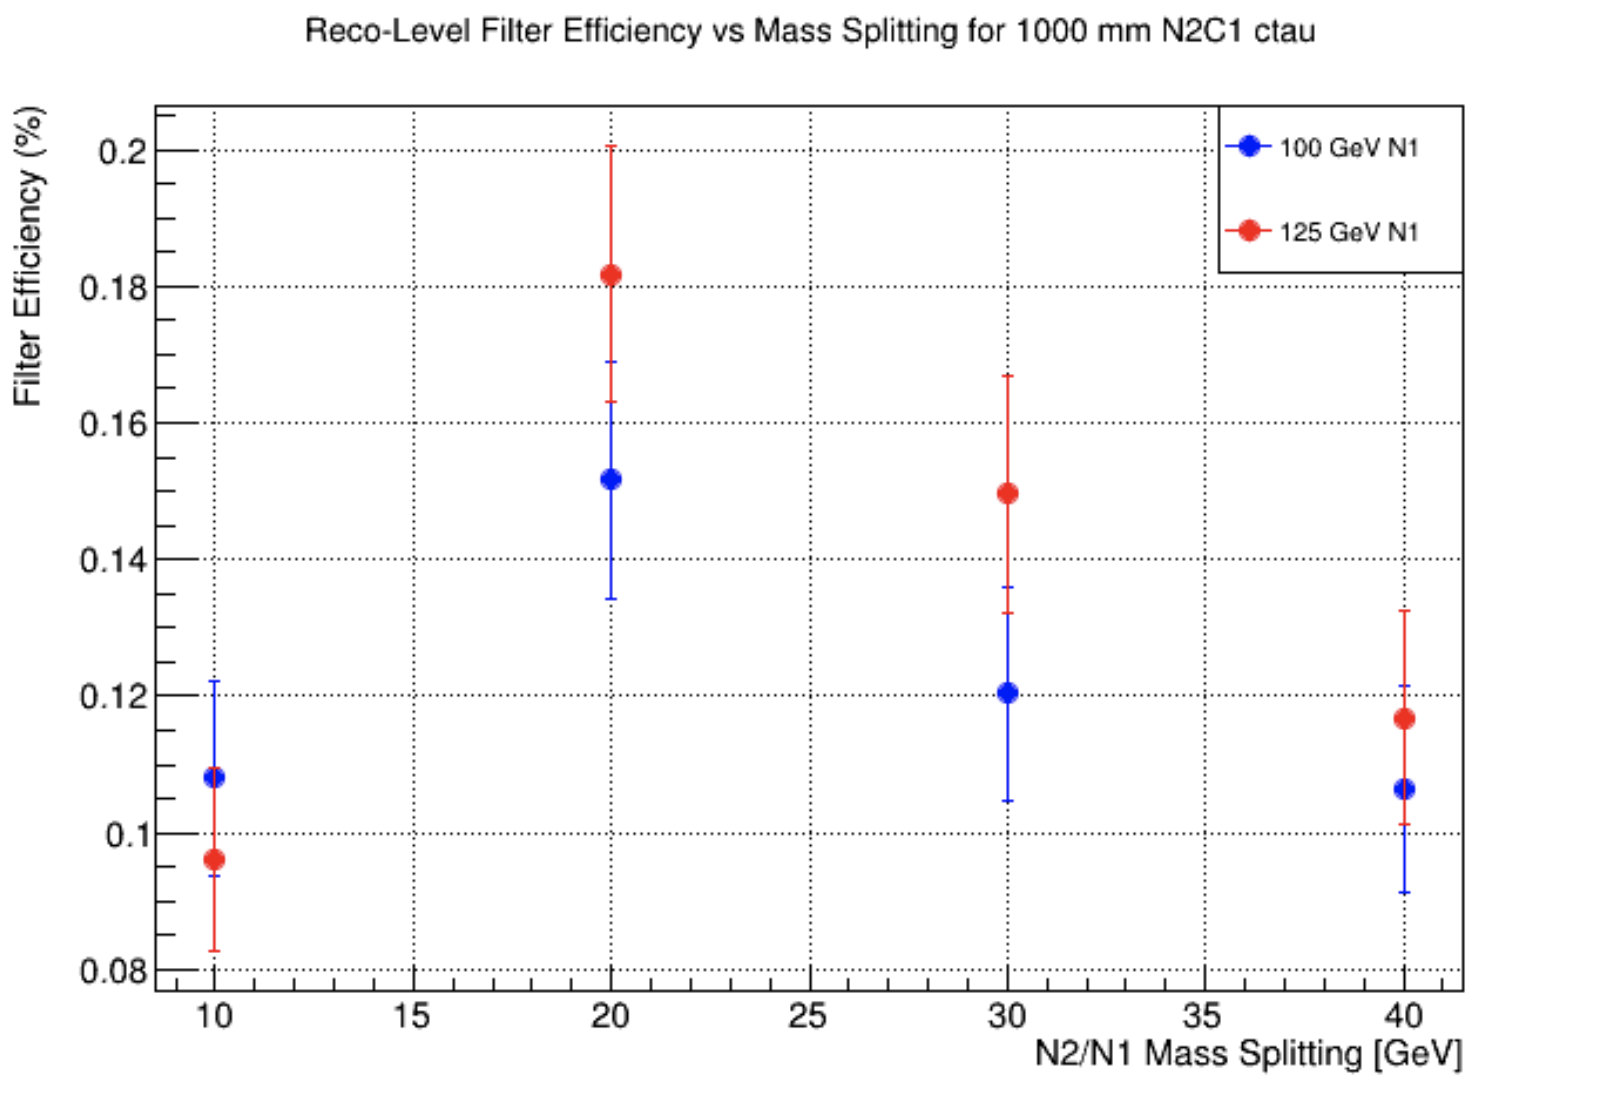
\includegraphics[width=.8\linewidth]{1000mmEff.png}  
  \caption{1000 mm ctau}
  \label{fig:sub-fourth18}
\end{subfigure}
\caption{Reco-Level Efficiency for fixed ctau in Higgsino Samples}
\label{fig:24}
\end{figure}
\par
For the Wino/Bino case, figure~\ref{fig:25} shows the events in the signal region for a given $\chi_{2}^{0}$ mass, while figure~\ref{fig:26} shows the events for a fixed ctau.
\par
\begin{figure} [H]
\begin{subfigure}{.5\textwidth}
  \centering
  % include first image
  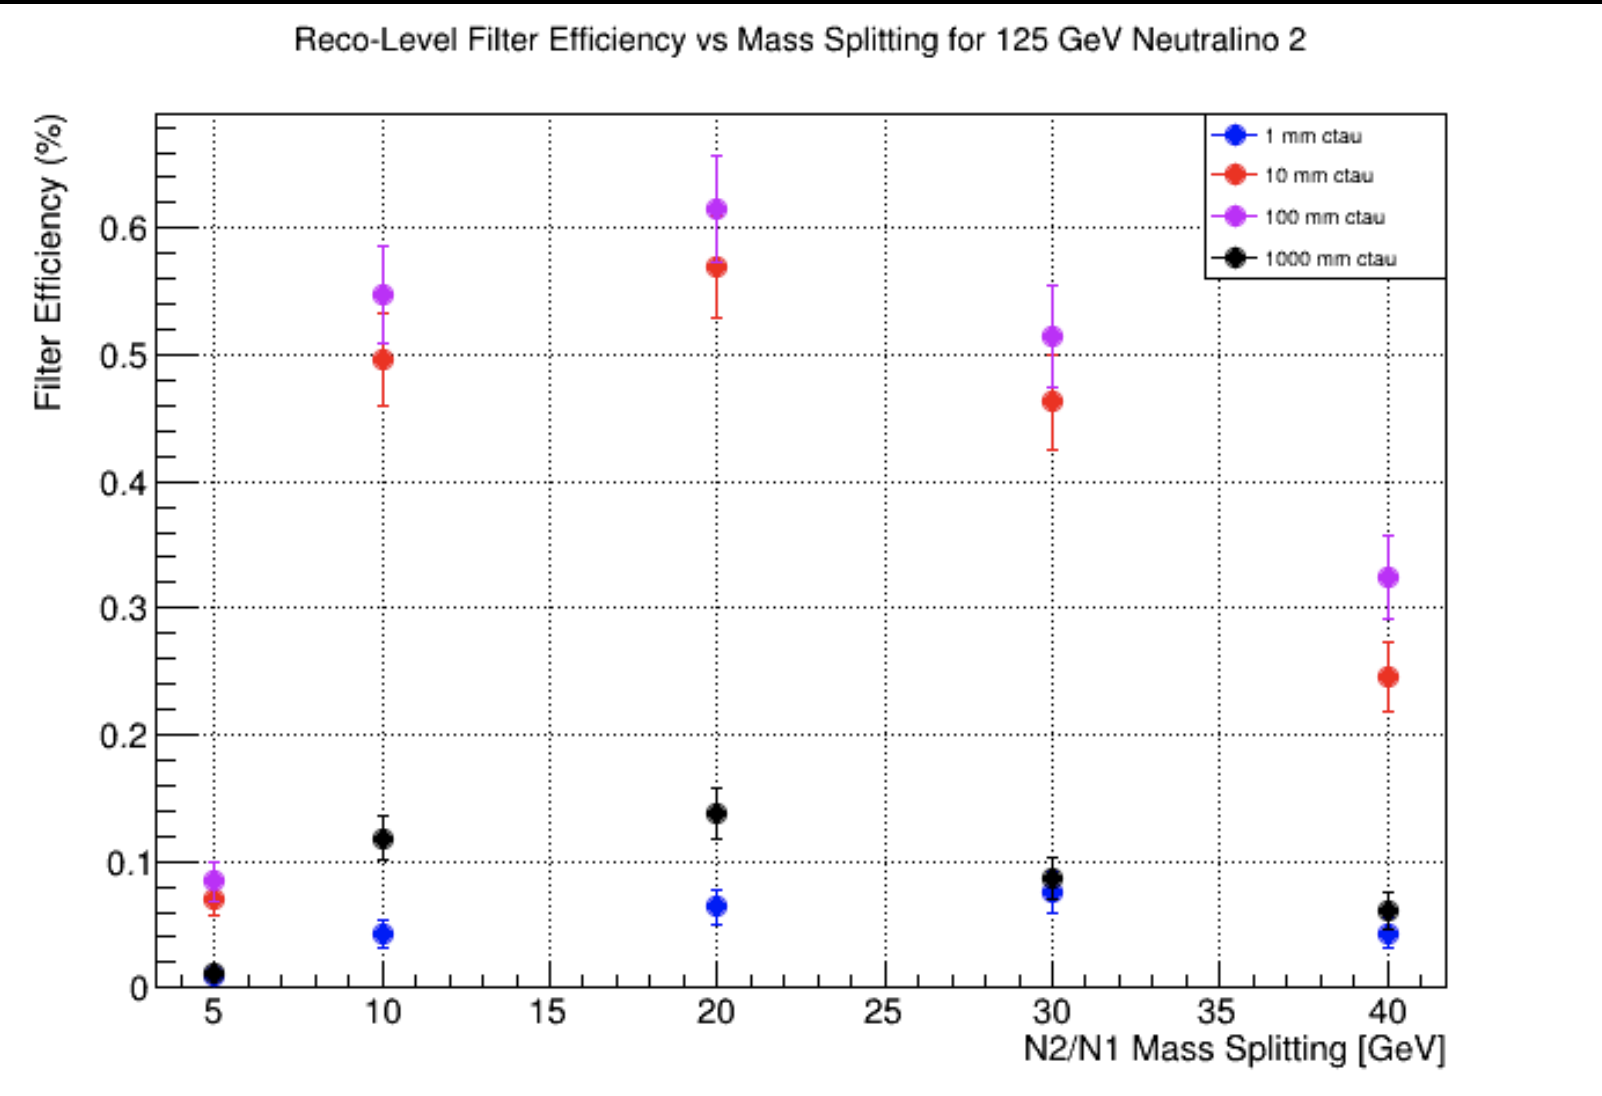
\includegraphics[width=.8\linewidth]{125GeVWinoEff.png}  
  \caption{125 GeV $\chi_{2}^{0}$}
  \label{fig:sub-first19}
\end{subfigure}
\begin{subfigure}{.5\textwidth}
  \centering
  % include second image
  \includegraphics[width=.8\linewidth]{150GeVWinoEff.png}  
  \caption{$\chi_{2}^{0}$ Wino/Bino}
  \label{fig:sub-second19}
\end{subfigure}
\caption{Reco-Level Efficiency for fixed $\chi_{2}^{0}$ mass in Wino/Bino Samples}
\label{fig:25}
\end{figure}

\begin{figure} [H]
\begin{subfigure}{.5\textwidth}
  \centering
  % include first image
  \includegraphics[width=.8\linewidth]{1mmWinoEff.png}  
  \caption{1 mm ctau}
  \label{fig:sub-first18}
\end{subfigure}
\begin{subfigure}{.5\textwidth}
  \centering
  % include second image
  \includegraphics[width=.8\linewidth]{10mmWinoEff.png}  
  \caption{10 mm ctau}
  \label{fig:sub-second18}
\end{subfigure}
\begin{subfigure}{.5\textwidth}
  \centering
  % include third image
  \includegraphics[width=.8\linewidth]{100mmWinoEff.png}  
  \caption{100 mm ctau}
  \label{fig:sub-third18}
\end{subfigure}
\begin{subfigure}{.5\textwidth}
  \centering
  % include fourth image
  \includegraphics[width=.8\linewidth]{1000mmWinoEff.png}  
  \caption{1000 mm ctau}
  \label{fig:sub-fourth18}
\end{subfigure}
\caption{Reco-Level Efficiency for fixed ctau in Wino/Bino Samples}
\label{fig:26}
\end{figure}
\par
As expected, the overall reco-level efficiency for a 10 and 100 mm ctau is far greater than that of the 1 and 1000 mm ctau. However, there are also meaningful differences in efficiency for different neutralino masses. For example, in both the Higgsino and Wino/Bino scenarios with a 20 GeV mass splitting and 10 mm and 100 mm ctaus, the sample with a heavier neutralinos enjoys a discernibly better filter efficiency than the 125 GeV $\chi_{2}^{0}$ sample. For a 100 cm ctau in the Wino/Bino scenario, a 40 GeV mass splitting corresponds with a particularly distinct difference in efficiency between the two samples. A heavier $\chi_{2}^{0}$ corresponds with more energy that can be distributed between the $\chi_{1}^{0}$ and the muons. Though most of the ``additional" energy from the heavier $\chi_{2}^{0}$ leads to a higher pT $\chi_{1}^{0}$, perhaps the additional energy of the muons leave a more distinct signal in the tracker and better reconstruction in general - allowing more events to pass the applied cuts. We could also compare efficiencies for each samples cut-by-cut, and determine if there is a particular selection that favors heavier neutralinos. Again, the initial theoretical cross-sections of the lighter neutralino processes is larger than those of the heavier neutralinos, so the smaller efficiency is largely unnoticeable.
\subsection{Conclusions and Future Steps}
In this study, we were largely successful in what we sought to achieve: discern a clear signal region for an electroweak SUSY process to which we expect CMS searches to be sensitive. However, there are many ways to make this search more complete and be more sensitive to a wider range of physical processes.
\par
As specified earlier in this note, the mixing of the mass eigenstates, which can lead to either a ``Higgsino-like" or a ``Wino/Bino-like" electroweakino, affects the shape of the dilepton mass distribution, as we illustrated in figure~\ref{fig:4}. In this study, we used the labels ``Higgsino" and ``Wino/Bino" to determine physically conceivable mass configurations and whether we needed to compute both the N2C1 and N2N1 processes (Higgsino) or just the "N2C1" case
(Wino/Bino). We would have produced more accurate dimuon mass plots and compute a correspondingly more accurate value for the expected number of events had we reshaped our distributions and reweighted our events to be consistent with figure~\ref{fig:4}.
\par
We also incurred a variety of computational inefficiencies throughout event generation. We lost over 50\% of events before applying generator-level cuts, likely due to jet-matching efficiencies and other inconsistencies at the interface of Madgraph and Pythia. It would have been more efficient to conduct an initial investigation regarding to optimal values for various parameters in Madgraph and Pythia, such as the XQCUT and the QCUT. Moreover, the event production procedure, starting from Madgraph's template cards to a finished set of nTuples, takes several days from start to finish. This greatly reduces our ability to create interesting samples with more neutralino masses and mass splittings, and it is possible that instructive trends in the data were missed as a result. I believe our code can be optimized to produce samples in a much shorter time.
\par
Lastly, a study of simulated SUSY processes and MC-generated data is largely unimportant if similar phenomena are not observed in real data. It would be illuminating to take data collected at CMS during 2018 or all of Run 2, and apply the set of reconstruction-level cuts that we did to our MC-generated SUSY processes. If similar dimuon mass distributions are observed in data, it is certainly worthwhile to further investigate these types of electoweak SUSY models. However, if there is no evidence of a signal in these regions, perhaps these models can be excluded, and significant time and effort can be devoted to other studies. In either case, SUSY presents an intuitive and clean solution to the hierarchy problem, and any efforts that allow us to better understand the relationship between supersymmetry and detector-level phenomena is interesting and informative.



\section{References}
\bibliographystyle{IEEE}
\bibliography{main}
\medskip 
\par \noindent
[1] D. J. Griffiths, Introduction to elementary particles. Wiley-VCH, 2020. \\
\par \noindent
[2] Particle Data Group. [Online]. Available: https://pdg.lbl.gov/. [Accessed: 20-May-2022]. \\
\par\noindent
[3] G. F. Giudice, “Naturally speaking: The naturalness criterion and physics at the LHC,” Perspectives on LHC Physics, pp. 155–178, 2008. \\
\par \noindent
[4] S. P. Martin, “A supersymmetry primer,” Perspectives on Supersymmetry, pp. 1–98, 1998. \\
\par \noindent
[5] C. Csáki and P. Tanedo, “Beyond the Standard Model,” 2013 European School of High-Energy Physics, pp. 169–268, Jun. 2015. \\
\par \noindent
[6] S. P. Martin, “Introduction to supersymmetry” 18-May-2019. [Online]. Available: https://www.niu.edu/spmartin/preSUSY2019\_Martin.pdf. [Accessed: 20-May-2022]. \\
\par \noindent
[7] R. N. Mohapatra, “Supersymmetry and R-parity: an Overview,” Richard Arnowitt Memorial Volume, pp. 1–21, Mar. 2015. \\
\par \noindent
[8] N. Arkani-Hamed, A. Delgado, and G. F. Giudice, “The well-tempered Neutralino,” Nuclear Physics B, vol. 741, no. 1-2, pp. 108–130, 2006. \\
\par \noindent
[9] The CMS Collaboration, “Search for supersymmetry in final states with two or three soft leptons and missing transverse momentum in proton-proton collisions at $\sqrt{s}$ = 13 TeV,” Journal of High Energy Physics, vol. 91, pp. 1–57, Apr. 2022. \\
\par \noindent
[10] S. J. Ling, University physics. volume 3. OpenStax College Rice University, 2016. \\
\par \noindent
[11] The CMS Collaboration, “Search for inelastic dark matter in events with two displaced muons and missing transverse momentum,” Internal Note, Jul. 2020. \\
\par \noindent
[12] The ATLAS Collaboration, "SUSY May 2020 Summary Plot Update," Internal Note, May. 2020. \\
\par \noindent
[13] B. Fuks, M. Klasen, D. Lamprea, M. Rothering, "Gaugino production in proton-proton collisions at a center-of-mass energy of 8 TeV," Journal of High Energy Physics, vol. 10, pp. 81, 2012. \\
\par \noindent
[14] B. Fuks, M. Klasen, D. Lamprea, M. Rothering, "Precision predictions for electroweak superpartner production at hadron colliders with {\textbackslash sc Resummino}," Eur. Phys. J. C, vol. 73, pp. 2480, 2013. \\
\par \noindent
[15] A. George, "What the Hell is Matchinng," HEP.UCSB.EDU/PEOPLE/CAG/MATCHING.PDF. \\
\par \noindent 
[16] C. Blocker, "Uncertainties on Efficiencies," CDF/MEMO/STATISTICS/PUBLIC/7168, Aug. 2004. \\
\end{document}